\subsection{Implementering}
%%%%%%%%%%%% MID WAY AGENDA %%%%%%%%%%%%%%
%\begin{frame}<beamer>
%\frametitle{Thomas Holm Pilgaard}
%\tableofcontents[currentsection]
%\end{frame}
%%%%%%%%%%%% MID WAY AGENDA %%%%%%%%%%%%%%


\begin{frame}{Indhold}{Jacob Naundrup Pedersen}
 \vfill\vfill\centering  
\begin{itemize}
	
\item Implementering \vspace{2mm}
\item Kontrol \vspace{2mm}
\item Resultater \vspace{2mm}
\item Diskussion/Konklusion \vspace{2mm}
\end{itemize}
 \vfill\vfill
\end{frame}


\begin{frame}{Implementering}{}
 \vfill\vfill\centering  
\begin{figure}[H]
\centering
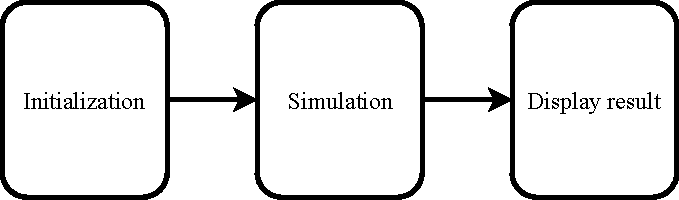
\includegraphics[width=0.75 \textwidth]{figures/Basic_implementation}
%\caption{Chosen structure of Simulering environment.}
\label{fig:Basic_Implementering}
\end{figure}
 \vfill\vfill

\end{frame}
%\subsection{Initialisering}
\begin{frame}{Implementering}{Initialisering}
    
\begin{table}[H]
\begin{enumerate} 
	\item Rør
	\begin{itemize}
		\item Længde [m]
		\item Sektioner 
		\item $\text{S}_\text{b}$ (Hældning) [\textperthousand]
		\item $\Delta$x = Længde/Sektioner [m]
		\item Diameter [m]
		\item Theta 
		\item $\text{Q}_{\text{f}}$[$\text{m}^\text{3}/\text{s}$]
		\item Side inflow  
		\item Placering i data 
	\end{itemize}
	\item Tank
	\begin{itemize}
		\item Størrelse [$\text{m}^\text{3}$]
		\item Højde [m]
		\item Areal = Størrelse / Højde [$\text{m}^\text{2}$]
		\item Maksimum outflow [$\text{m}^\text{3}/\text{s}$]
		\item Placering i data 
	\end{itemize}
	
\end{enumerate}
%\caption{List of parameters for pipe and tank.}
\label{tab:init_list}
\end{table}

\end{frame}


% \begin{frame}{Implementering}{Initialisering}
%  \vfill\vfill\centering  
%  \begin{itemize}
%  	\item Rør specifikationer
%  \end{itemize}
% \begin{figure}[!h]
% \centering
% 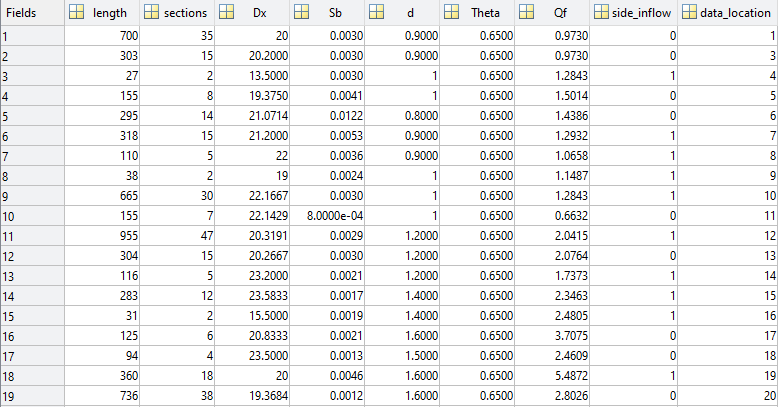
\includegraphics[width=0.97 \textwidth]{figures/Fredericia_pipe_setup2.PNG}
% %\caption{Setup in MATLAB of pipe specification of the main line in Fredericia.}
% \label{fig:Fredericia_pipe_setup}
% \end{figure}
%  \vfill\vfill

% \end{frame}

% \begin{frame}{Implementering}{Initialisering}
%  \vfill\vfill\centering  
%  \begin{itemize}
%  	\item Tank specifikationer 
%  \end{itemize}
%     \begin{figure}[H]
% \centering
% 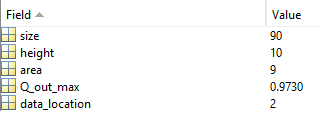
\includegraphics[width=0.5 \textwidth]{figures/tank_spec}
% %\caption{Setup in MATLAB of tank specifications.}
% \label{fig:Fredericia_pipe_setup}
% \end{figure}
%  \vfill\vfill
% \end{frame}

\begin{frame}{Implementering}{Initialisering}
     \vfill\vfill\centering  
     \begin{itemize}
     	\item Steady state
     	\item System opsætning
     \end{itemize}
\begin{figure}[H]
\centering
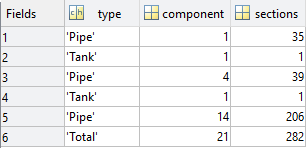
\includegraphics[width=0.4 \textwidth]{figures/sys_setup_matlab.png}
%\caption{Display of structure showing system setup information in MATLAB.}
\label{fig:sys_setup_matlab}
\end{figure}
 \vfill\vfill
\end{frame}

% \begin{frame}{Implementering}{Initialisering}
%  \vfill\vfill\centering  
%     \begin{figure}[H]
%  \centering
%  % This file was created by matlab2tikz.
%
%The latest updates can be retrieved from
%  http://www.mathworks.com/matlabcentral/fileexchange/22022-matlab2tikz-matlab2tikz
%where you can also make suggestions and rate matlab2tikz.
%
\definecolor{mycolor1}{rgb}{0.00000,0.44700,0.74100}%
%
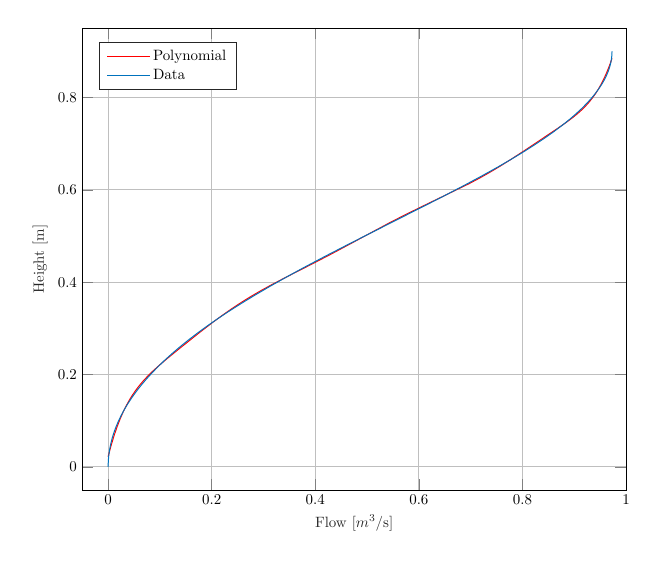
\begin{tikzpicture}[thick,scale=0.9, every node/.style={scale=0.6}]

\begin{axis}[%
width=3.021in,
height=2.566in,
at={(0.758in,0.481in)},
scale only axis,
xmin=-0.05,
xmax=1,
xlabel style={font=\color{white!15!black}},
xlabel={Flow [$\text{m}^\text{3}$/s]},
ymin=-0.05,
ymax=0.95,
ylabel style={font=\color{white!15!black}},
ylabel={Height [m]},
axis background/.style={fill=white},
xmajorgrids,
ymajorgrids,
legend style={at={(0.03,0.97)}, anchor=north west, legend cell align=left, align=left, draw=white!15!black}
]
\addplot [color=red]
  table[row sep=crcr]{%
0	0.0222641876397454\\
0.00583788013141662	0.0468505124572859\\
0.0116757602628333	0.0685037472280541\\
0.01751364039425	0.0875962984430564\\
0.0233515205256666	0.104462594043742\\
0.0291894006570832	0.119402060847026\\
0.0350272807884998	0.132681928352076\\
0.0408651609199165	0.14453986606579\\
0.0467030410513332	0.155186461298207\\
0.0535139012046525	0.166323129330026\\
0.0603247613579719	0.176319581381477\\
0.0681086015331941	0.186627394570619\\
0.0768654217303191	0.1971234679247\\
0.0865952219493469	0.207784706738995\\
0.0982709822121801	0.219634930070442\\
0.113838662562624	0.23449066785112\\
0.138163163110194	0.256755738358134\\
0.176109383964402	0.290671244351543\\
0.201406864533874	0.312526360051635\\
0.221839444993832	0.329374050052282\\
0.240326065409985	0.34381856012056\\
0.257839705804235	0.35673446219757\\
0.275353346198485	0.368905237211488\\
0.293839966614638	0.381009693497422\\
0.314272547074596	0.393647570538794\\
0.339570027644068	0.408528726872221\\
0.390164988783012	0.437347221406009\\
0.429084189659123	0.459928516339826\\
0.468003390535234	0.483262809711989\\
0.54389583224365	0.528968698128539\\
0.574058212922636	0.546263994393304\\
0.604220593601622	0.562860267064146\\
0.696653695682386	0.613119065583713\\
0.717086276142344	0.62530025086964\\
0.736545876580399	0.637586486102553\\
0.756005477018455	0.650574852430809\\
0.777411037500316	0.665605335087019\\
0.803681498091691	0.684833203666043\\
0.864979239471565	0.730734878672607\\
0.884438839909621	0.745858014555948\\
0.897087580194357	0.756440925031475\\
0.906817380413385	0.765353228191959\\
0.914601220588607	0.773208230042211\\
0.922385060763829	0.781942336734848\\
0.929195920917148	0.790515086732738\\
0.935033801048565	0.798722858348917\\
0.940871681179982	0.807888165233192\\
0.946709561311398	0.818188953039921\\
0.952547441442815	0.829827057099856\\
0.958385321574232	0.8430304635012\\
0.963250221683745	0.855413188684596\\
0.968115121793259	0.869225396536382\\
0.972980021902773	0.884648045759077\\
};
\addlegendentry{Polynomial}

\addplot [color=mycolor1]
  table[row sep=crcr]{%
0	0\\
0.00030642296001504	0.01233\\
0.00122592449248948	0.02466\\
0.00275919619829157	0.03699\\
0.00492531381189298	0.04941\\
0.00771691837291222	0.0618300000000001\\
0.0111359602571995	0.07425\\
0.0152163500161991	0.0867600000000001\\
0.0199744759873318	0.09936\\
0.02542711466865	0.11205\\
0.0315913434853029	0.12483\\
0.0384338333138317	0.13761\\
0.0460682367603654	0.15057\\
0.0544660114484651	0.16362\\
0.0637094855914684	0.17685\\
0.0738302832003164	0.19026\\
0.0847840346449592	0.20376\\
0.0967472281174419	0.21753\\
0.109678802055319	0.23148\\
0.123697951078652	0.2457\\
0.138846482140551	0.26019\\
0.155163670747372	0.27495\\
0.172793050923732	0.29007\\
0.191782482726017	0.30555\\
0.212292745916907	0.32148\\
0.234499027859045	0.33795\\
0.25845887409398	0.35496\\
0.284486130286045	0.37269\\
0.312918691318617	0.39132\\
0.344254168236911	0.41112\\
0.37915911064623	0.43245\\
0.419079139891965	0.45612\\
0.466907719593891	0.48375\\
0.53413117460992	0.52182\\
0.638838688603708	0.58113\\
0.684244287950606	0.60759\\
0.720760960442891	0.62955\\
0.751794914662872	0.6489\\
0.778966712722586	0.66654\\
0.802970121524758	0.68283\\
0.824328787062596	0.69804\\
0.843524532554507	0.71244\\
0.860764663768599	0.72612\\
0.87624717181071	0.73917\\
0.890156294853092	0.75168\\
0.902569357193314	0.76365\\
0.913654569164784	0.77517\\
0.923559217305502	0.78633\\
0.93233869141443	0.79713\\
0.94005219868443	0.80757\\
0.946818481487701	0.81774\\
0.952682361805689	0.82764\\
0.957734233356883	0.83736\\
0.962003234496279	0.8469\\
0.9655201136824	0.85626\\
0.968316966985129	0.86544\\
0.97044491415244	0.87453\\
0.971919271555091	0.88353\\
0.972756442059394	0.89244\\
0.972980021902773	0.9\\
};
\addlegendentry{Data}

\end{axis}
\end{tikzpicture}%
% %\caption{}
% \label{fig:curvefit_comparision}
% \end{figure}
%  \vfill\vfill
% \end{frame}

% \begin{frame}{Implementering}{Initialisering}
% \begin{figure}[H]
%  \centering
%  % This file was created by matlab2tikz.
%
%The latest updates can be retrieved from
%  http://www.mathworks.com/matlabcentral/fileexchange/22022-matlab2tikz-matlab2tikz
%where you can also make suggestions and rate matlab2tikz.
%
\definecolor{mycolor1}{rgb}{0.00000,0.44700,0.74100}%
%
\begin{tikzpicture}

\begin{axis}[%
width=1.268in,
height=3.175in,
at={(2.2in,1.103in)},
scale only axis,s
xmin=-0.05,
xmax=0.255,
xlabel style={font=\color{white!15!black}},
xlabel={Flow [$\text{m}^\text{3}$/s]},
ymin=-0.05,
ymax=0.4,
ylabel style={font=\color{white!15!black}},
ylabel={Height [m]},
axis background/.style={fill=white},
xmajorgrids,
ymajorgrids,
legend style={at={(0.03,0.97)}, anchor=north west, legend cell align=left, align=left, draw=white!15!black}
]
\addplot [color=red]
  table[row sep=crcr]{%
0	0.0222641876397452\\
0.002	0.0310423507186317\\
0.004	0.0394452957735427\\
0.00600000000000001	0.0474896123161433\\
0.00800000000000001	0.0551913093444532\\
0.01	0.0625658308096022\\
0.012	0.0696280707783006\\
0.014	0.076392388295221\\
0.016	0.0828726219494472\\
0.018	0.0890821041491136\\
0.02	0.0950336751083192\\
0.022	0.100739696550368\\
0.024	0.106212065131344\\
0.026	0.111462225588011\\
0.028	0.11650118361396\\
0.03	0.121339518467939\\
0.032	0.125987395318202\\
0.034	0.130454577326758\\
0.036	0.134750437477274\\
0.038	0.138883970150443\\
0.04	0.142863802450524\\
0.042	0.146698205286753\\
0.044	0.150395104213308\\
0.046	0.153962090031438\\
0.048	0.15740642915736\\
0.05	0.16073507375949\\
0.052	0.163954671668528\\
0.054	0.167071576063904\\
0.056	0.170091854940031\\
0.058	0.17302130035581\\
0.06	0.175865437470771\\
0.062	0.178629533371213\\
0.064	0.181318605689683\\
0.066	0.183937431021079\\
0.068	0.186490553138647\\
0.07	0.188982291013104\\
0.072	0.191416746638089\\
0.075	0.194969485627572\\
0.078	0.198414344321734\\
0.081	0.201762648867287\\
0.084	0.20502481071003\\
0.087	0.208210377368781\\
0.09	0.211328081265009\\
0.093	0.214385886658126\\
0.097	0.218382201981612\\
0.101	0.222300129592964\\
0.105	0.226152997837096\\
0.11	0.230894979828061\\
0.116	0.236501118023782\\
0.123	0.24295746024834\\
0.131	0.250261133339763\\
0.141	0.259319049720577\\
0.153	0.270116802578941\\
0.164	0.279948128414307\\
0.173	0.287930045688142\\
0.181	0.294962503821962\\
0.188	0.301055217728628\\
0.195	0.307080190139537\\
0.201	0.312182600461743\\
0.207	0.317221300531533\\
0.213	0.322190515539783\\
0.219	0.327085077941444\\
0.224	0.331103612243363\\
0.229	0.33506502224299\\
0.234	0.338967534353605\\
0.239	0.342809785047988\\
0.244	0.346590827426471\\
0.249	0.35031013183293\\
0.254	0.353967581129179\\
0.256	0.35541329220446\\
};
\addlegendentry{Curve fit}

\addplot [color=mycolor1]
  table[row sep=crcr]{%
0	0\\
2.48304185804238e-05	0.00351000000000001\\
9.93232085852447e-05	0.00702000000000003\\
0.000223482969415489	0.01053\\
0.000397317355443627	0.01404\\
0.000620837059076784	0.01755\\
0.000894055787063641	0.02106\\
0.00122592449248948	0.02466\\
0.00161011236359732	0.02826\\
0.00204664383847447	0.03186\\
0.0025355465084787	0.03546\\
0.00307685105291455	0.03906\\
0.00367059116604707	0.04266\\
0.0043168034765097	0.04626\\
0.00501552745916467	0.04986\\
0.00576680533948298	0.05346\\
0.00657068199051475	0.05706\\
0.00742720482252818	0.06066\\
0.00833642366539827	0.06426\\
0.00929839064383481	0.06786\\
0.0103131600455422	0.07146\\
0.0113807881824109	0.07506\\
0.0125013332448436	0.07866\\
0.0136748551493265	0.08226\\
0.0149014153793596	0.08586\\
0.0161810768198663	0.08946\\
0.0175139035852057	0.09306\\
0.0188999608409186	0.09666\\
0.0203393146193402	0.10026\\
0.0218700338511926	0.10395\\
0.0234568901890829	0.10764\\
0.0250999562933016	0.11133\\
0.0267993048905982	0.11502\\
0.0285550085329623	0.11871\\
0.0303671393503522	0.1224\\
0.0322357687975712	0.12609\\
0.0341609673954891	0.12978\\
0.0361428044668208	0.13347\\
0.0381813478666689	0.13716\\
0.0403284787506254	0.14094\\
0.042535254094141	0.14472\\
0.0448017402173691	0.1485\\
0.0471280005690068	0.15228\\
0.0495140953962901	0.15606\\
0.0519600814105286	0.15984\\
0.0544660114484651	0.16362\\
0.0570319341297459	0.1674\\
0.0597211484251551	0.17127\\
0.0624733342640793	0.17514\\
0.0652885277920768	0.17901\\
0.06816675896115	0.18288\\
0.0711080511274374	0.18675\\
0.0741124206465261	0.19062\\
0.0772519632947214	0.19458\\
0.0804575616887742	0.19854\\
0.0837292079118647	0.2025\\
0.0870668845587141	0.20646\\
0.0904705642744617	0.21042\\
0.093940209293403	0.21438\\
0.0975568902819463	0.21843\\
0.101242453855357	0.22248\\
0.104996822806891	0.22653\\
0.108819906506757	0.23058\\
0.112798860871919	0.23472\\
0.116849381300941	0.23886\\
0.120971324178149	0.243\\
0.125164529004631	0.24714\\
0.129522307794482	0.25137\\
0.133954085548652	0.2556\\
0.138459632885561	0.25983\\
0.143038699635108	0.26406\\
0.147790793375852	0.26838\\
0.152618972114771	0.2727\\
0.157522898470217	0.27702\\
0.162606744485203	0.28143\\
0.16776873600719	0.28584\\
0.173008431171206	0.29025\\
0.178434668332884	0.29475\\
0.183940789913321	0.29925\\
0.189526230350682	0.30375\\
0.195304472276872	0.30834\\
0.201163941357038	0.31293\\
0.207221197384301	0.31761\\
0.213361364393635	0.32229\\
0.2197040632307	0.32706\\
0.226131092492676	0.33183\\
0.23276510614099	0.33669\\
0.239484561913134	0.34155\\
0.246415106055723	0.3465\\
0.253560216377759	0.35154\\
0.255102805548652	0.35262\\
};
\addlegendentry{Raw data}

\end{axis}

\begin{axis}[%
width=1.268in,
height=3.175in,
at={(4.216in,1.103in)},
scale only axis,
xmin=0.25,
xmax=0.75,
xlabel style={font=\color{white!15!black}},
xlabel={Flow [$\text{m}^\text{3}$/s]},
ymin=0.3,
ymax=0.7,
ylabel style={font=\color{white!15!black}},
%ylabel={y},
axis background/.style={fill=white},
xmajorgrids,
ymajorgrids,
legend style={at={(0.03,0.97)}, anchor=north west, legend cell align=left, align=left, draw=white!15!black}
]
\addplot [color=red]
  table[row sep=crcr]{%
0.249	0.35031013183293\\
0.255	0.354691666581612\\
0.262	0.359691701230937\\
0.269	0.364573586617454\\
0.276	0.369340965039136\\
0.283	0.373998737951873\\
0.29	0.378552926883383\\
0.297	0.383010521588671\\
0.305	0.387996670089977\\
0.313	0.392879507167007\\
0.322	0.398265932720645\\
0.332	0.404141450374147\\
0.343	0.410502990594094\\
0.357	0.418499578118555\\
0.401	0.443559700309453\\
0.415	0.451667310051688\\
0.428	0.459288735165773\\
0.442	0.467597762950332\\
0.457	0.476603835082106\\
0.476	0.488120525887873\\
0.515	0.511793040483264\\
0.529	0.520176602179741\\
0.541	0.527271293048054\\
0.552	0.533686029865968\\
0.563	0.540007271687931\\
0.574	0.546231314734744\\
0.585	0.552359493128402\\
0.597	0.558943399249206\\
0.61	0.56597490588983\\
0.626	0.574529055842827\\
0.658	0.59160882368966\\
0.67	0.59812620199676\\
0.68	0.603653211457091\\
0.689	0.608723309841312\\
0.697	0.613319949398277\\
0.705	0.618011892679499\\
0.713	0.622807955472417\\
0.72	0.627095546670148\\
0.727	0.631471829860599\\
0.734	0.635939028034652\\
0.741	0.64049797219494\\
0.748	0.645148024720358\\
0.751	0.647168315462028\\
};
\addlegendentry{Curve fit}

\addplot [color=mycolor1]
  table[row sep=crcr]{%
0.249976576240672	0.34902\\
0.259236020098798	0.3555\\
0.268770604516453	0.36207\\
0.278582982727352	0.36873\\
0.288810967283916	0.37557\\
0.299324710559653	0.3825\\
0.310264902062615	0.38961\\
0.321496592023219	0.39681\\
0.333162969488798	0.40419\\
0.345413837726718	0.41184\\
0.358111484464603	0.41967\\
0.371406904414949	0.42777\\
0.385306199342518	0.43614\\
0.399965417403482	0.44487\\
0.415544526316372	0.45405\\
0.432206111207128	0.46377\\
0.450269978113671	0.47421\\
0.470216918454365	0.48564\\
0.493006156351848	0.4986\\
0.521512531670953	0.51471\\
0.610182365254768	0.56475\\
0.631784954161493	0.57708\\
0.650385062883746	0.58779\\
0.667102191938927	0.59751\\
0.682417982952271	0.60651\\
0.696652221286361	0.61497\\
0.709967603587233	0.62298\\
0.722523515471217	0.63063\\
0.734329931889074	0.63792\\
0.745542001375896	0.64494\\
0.750094863039869	0.64782\\
};
\addlegendentry{Raw data}

\end{axis}

\begin{axis}[%
width=1.268in,
height=3.175in,
at={(6.032in,1.103in)},
scale only axis,
xmin=0.75,
xmax=1,
xlabel style={font=\color{white!15!black}},
xlabel={Flow [$\text{m}^\text{3}$/s]},
ymin=0.6,
ymax=1,
ylabel style={font=\color{white!15!black}},
%ylabel={y},
axis background/.style={fill=white},
xmajorgrids,
ymajorgrids,
legend style={at={(0.03,0.97)}, anchor=north west, legend cell align=left, align=left, draw=white!15!black}
]
\addplot [color=red]
  table[row sep=crcr]{%
0.749	0.64581964896121\\
0.754	0.649204708850327\\
0.759	0.652633625517857\\
0.765	0.656803751868769\\
0.771	0.661030811194417\\
0.777	0.665310362972644\\
0.783	0.669637308241325\\
0.79	0.674737739432043\\
0.798	0.680623882483808\\
0.807	0.687300479571666\\
0.819	0.696257588271415\\
0.855	0.723210485257116\\
0.864	0.729992748255671\\
0.87	0.734559402479318\\
0.875	0.7384106634497\\
0.879	0.741533242965855\\
0.883	0.744703664565781\\
0.887	0.747933741185847\\
0.89	0.750403574788058\\
0.893	0.752921066814172\\
0.896	0.755493360494214\\
0.899	0.75812830975509\\
0.902	0.760834523589958\\
0.904	0.762682870204443\\
0.906	0.764570050724757\\
0.908	0.766499235321348\\
0.91	0.768473775146326\\
0.912	0.770497209220108\\
0.914	0.772573271494007\\
0.916	0.77470589809123\\
0.918	0.776899234736596\\
0.92	0.779157644370867\\
0.922	0.78148571495197\\
0.924	0.783888267452656\\
0.926	0.78637036405471\\
0.928	0.788937316539267\\
0.93	0.791594694883246\\
0.932	0.794348336062853\\
0.934	0.797204353058196\\
0.936	0.800169144081827\\
0.938	0.803249402016365\\
0.94	0.806452124072433\\
0.942	0.809784621671747\\
0.944	0.813254530555241\\
0.946	0.816869821118178\\
0.948	0.820638808987019\\
0.95	0.824570165823802\\
0.952	0.828672930379062\\
0.954	0.832956519781786\\
0.956	0.83743074108508\\
0.958	0.842105803058818\\
0.96	0.84699232823691\\
0.961	0.849518325233025\\
0.962	0.852101365229253\\
0.963	0.85474289793944\\
0.964	0.857444401290818\\
0.965	0.860207381836799\\
0.966	0.863033375162934\\
0.967	0.865923946307994\\
0.968	0.868880690181764\\
0.969	0.871905231988518\\
0.97	0.874999227660777\\
0.971	0.878164364288391\\
0.972	0.88140236055983\\
0.973	0.884714967201509\\
0.974	0.888103967428042\\
0.975	0.891571177390592\\
0.976	0.895118446636695\\
0.977	0.898747658567163\\
0.978	0.902460730904545\\
0.979	0.906259616161808\\
0.98	0.910146302118012\\
0.981	0.914122812295408\\
0.982	0.918191206448008\\
0.983	0.922353581045962\\
0.984	0.926612069773207\\
0.985	0.930968844025068\\
0.986	0.935426113410837\\
0.987	0.939986126263528\\
0.988	0.944651170155241\\
0.989	0.94942357241077\\
0.99	0.954305700637324\\
0.991	0.959299963249688\\
0.992	0.964408810005519\\
0.993	0.969634732541658\\
0.994	0.974980264923291\\
0.995	0.980447984188683\\
0.996	0.986040510907197\\
0.997	0.991760509736736\\
0.998	0.997610689989807\\
0.999	1.00359380620654\\
};
\addlegendentry{Curve fit}

\addplot [color=mycolor1]
  table[row sep=crcr]{%
0.749953011619629	0.64773\\
0.757432493850936	0.6525\\
0.7645534467828	0.65709\\
0.771459426257282	0.66159\\
0.778152382292587	0.666\\
0.784634493295423	0.67032\\
0.79090814901061	0.67455\\
0.797107031793008	0.67878\\
0.80309959793141	0.68292\\
0.808888756653249	0.68697\\
0.814477574763368	0.69093\\
0.819993811294507	0.69489\\
0.825312955439522	0.69876\\
0.830438467149594	0.70254\\
0.835493438680027	0.70632\\
0.840358668167521	0.71001\\
0.845154044624885	0.7137\\
0.849763920653625	0.7173\\
0.854192243840763	0.72081\\
0.858554017076624	0.72432\\
0.862738926081918	0.72774\\
0.866858678348505	0.73116\\
0.870912317842577	0.73458\\
0.874794858436942	0.73791\\
0.878612967739068	0.74124\\
0.882265237414114	0.74448\\
0.885854942862714	0.74772\\
0.889381327910747	0.75096\\
0.892748344234666	0.75411\\
0.896054132353246	0.75726\\
0.899206212192649	0.76032\\
0.902299290844236	0.76338\\
0.905332781578393	0.76644\\
0.908219521283074	0.76941\\
0.911049066051665	0.77238\\
0.913820907745099	0.77535\\
0.916534547817645	0.77832\\
0.919109911384276	0.7812\\
0.921629650727206	0.78408\\
0.924093337843144	0.78696\\
0.926426187075666	0.78975\\
0.928705666434312	0.79254\\
0.930931411134825	0.79533\\
0.933103064562747	0.79812\\
0.935152834380352	0.80082\\
0.937151311834705	0.80352\\
0.939098196039214	0.80622\\
0.94099319357008	0.80892\\
0.942836018535166	0.81162\\
0.944567561425243	0.81423\\
0.946249847287773	0.81684\\
0.94788263829435	0.81945\\
0.949465703415043	0.82206\\
0.95099881846928	0.82467\\
0.952431467489442	0.82719\\
0.953817159863378	0.82971\\
0.955155712240545	0.83223\\
0.956446947384101	0.83475\\
0.95769069420742	0.83727\\
0.958886787809357	0.83979\\
0.95999488447617	0.84222\\
0.961058386582694	0.84465\\
0.962077162786354	0.84708\\
0.963051087201856	0.84951\\
0.96398003942538	0.85194\\
0.964863904557722	0.85437\\
0.965702573226402	0.8568\\
0.966495941606697	0.85923\\
0.967217019529645	0.86157\\
0.967895916613032	0.86391\\
0.968532554832599	0.86625\\
0.969126860996706	0.86859\\
0.969678766759406	0.87093\\
0.970188208632667	0.87327\\
0.970655127997724	0.87561\\
0.971079471115558	0.87795\\
0.971461189136518	0.88029\\
0.971800238109051	0.88263\\
0.972096578987574	0.88497\\
0.972350177639461	0.88731\\
0.972561004851152	0.88965\\
0.972729036333381	0.89199\\
0.97285425272553	0.89433\\
0.972936639599091	0.89667\\
0.972976187460251	0.89901\\
0.972980021902773	0.9\\
};
\addlegendentry{Raw data}

\end{axis}
\end{tikzpicture}%
% %\caption{}
% \label{fig:curvefit_comparision_split}
% \end{figure}


% \end{frame}



% \begin{frame}{Implementering}{Initialisering}
%  \vfill\vfill\centering  
%  \begin{figure}[H]
%  \centering
%  % This file was created by matlab2tikz.
%
%The latest updates can be retrieved from
%  http://www.mathworks.com/matlabcentral/fileexchange/22022-matlab2tikz-matlab2tikz
%where you can also make suggestions and rate matlab2tikz.
%
\definecolor{mycolor1}{rgb}{0.00000,0.44700,0.74100}%
\definecolor{mycolor2}{rgb}{0.85000,0.32500,0.09800}%
\definecolor{mycolor3}{rgb}{0.92900,0.69400,0.12500}%
\definecolor{mycolor4}{rgb}{0.49400,0.18400,0.55600}%
%
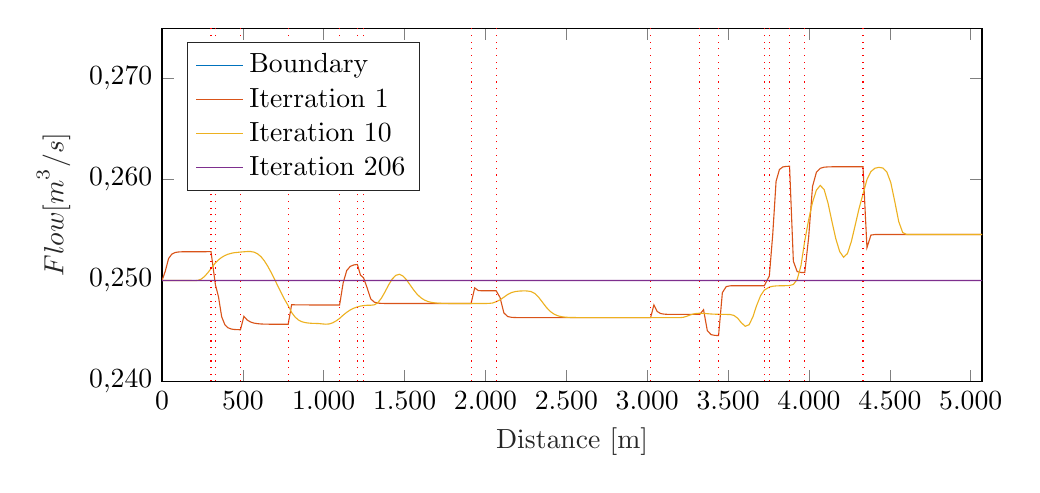
\begin{tikzpicture}

% \begin{axis}[%
% width=4.1in,
% height=1.7661in,
% at={(2.08in,4.154in)},
% scale only axis,
% xmin=0,
% xmax=5070,
% xlabel style={font=\color{white!15!black}},
% xlabel={Distance [m]},
% ymin=0.23,
% ymax=0.5,
% ylabel style={font=\color{white!15!black}},
% ylabel={Height [m]},
% y tick label style={
%         /pgf/number format/.cd,
%             fixed,
%             fixed zerofill,
%             precision=3,
%         /tikz/.cd  },
% axis background/.style={fill=white},
% title style={font=\bfseries},
% %title={Curvefit},
% legend style={legend cell align=left, align=left, draw=white!15!black}
% ]
% \addplot [color=mycolor1]
%   table[row sep=crcr]{%
% 0	0.351046566681362\\
% 303	0.351046566681362\\
% 303	0.335846494096586\\
% 330	0.335846494096586\\
% 330	0.309081835974212\\
% 485	0.309081835974212\\
% 485	0.252859425031602\\
% 780	0.252859425031602\\
% 780	0.30113200759115\\
% 1098	0.30113200759115\\
% 1098	0.334449091811621\\
% 1208	0.334449091811621\\
% 1208	0.356846112954372\\
% 1246	0.356846112954372\\
% 1246	0.335846494096586\\
% 1911	0.335846494096586\\
% 1911	0.471158308282611\\
% 2066	0.471158308282611\\
% 2066	0.31921912278267\\
% 3021	0.31921912278267\\
% 3021	0.316751000824297\\
% 3325	0.316751000824297\\
% 3325	0.344573805215077\\
% 3441	0.344573805215077\\
% 3441	0.349812515584745\\
% 3724	0.349812515584745\\
% 3724	0.341336368817792\\
% 3755	0.341336368817792\\
% 3755	0.326099272523606\\
% 3880	0.326099272523606\\
% 3880	0.366998098881595\\
% 3974	0.366998098881595\\
% 3974	0.268429914892295\\
% 4334	0.268429914892295\\
% 4334	0.369764380792731\\
% 5070	0.369764380792731\\
% };
% \addlegendentry{Boundary}

% \addplot [color=mycolor2]
%   table[row sep=crcr]{%
% 0	0.351046566681362\\
% 20.1999999999998	0.34968895516522\\
% 40.3999999999996	0.350569191323302\\
% 60.6000000000004	0.350878440171073\\
% 80.8000000000002	0.350987324814923\\
% 121.2	0.351039206755559\\
% 303	0.351046566320292\\
% 303	0.337920017091164\\
% 330	0.337104830155113\\
% 330	0.308816288287744\\
% 349.375	0.311112987536944\\
% 368.75	0.309891138768762\\
% 388.125	0.309403535853562\\
% 407.5	0.309209591216131\\
% 426.875	0.309132551677067\\
% 485	0.309085006824716\\
% 485	0.250256817505033\\
% 506.071428571428	0.253261105530328\\
% 527.142857142857	0.253071711576922\\
% 548.214285714286	0.25297158569083\\
% 590.357142857143	0.252890721389122\\
% 695.714285714286	0.25286070441507\\
% 780	0.252859526163775\\
% 780	0.29830065184251\\
% 801.2	0.301150556440007\\
% 907.2	0.30113221456395\\
% 1098	0.301132007618435\\
% 1098	0.332701121968967\\
% 1120	0.333213670339319\\
% 1142	0.334029438639845\\
% 1164	0.334306307291627\\
% 1186	0.334400486116465\\
% 1208	0.334432545507298\\
% 1208	0.358081245261019\\
% 1227	0.357124156438658\\
% 1246	0.356938719651225\\
% 1246	0.336046212403744\\
% 1268.16666666667	0.3368923261296\\
% 1290.33333333333	0.336155393261834\\
% 1312.5	0.335937573806405\\
% 1334.66666666667	0.335873335453471\\
% 1401.16666666667	0.335847180709607\\
% 1911	0.335846494096586\\
% 1911	0.469052641075905\\
% 1933.14285714286	0.471444240967685\\
% 1955.28571428571	0.471182537374261\\
% 2021.71428571429	0.471158322977317\\
% 2066	0.471158308388112\\
% 2066	0.318622019097347\\
% 2089.875	0.320496612934221\\
% 2113.75	0.319514616894594\\
% 2137.625	0.319287270193854\\
% 2185.375	0.319222740165969\\
% 2591.25	0.31921912278267\\
% 3021	0.31921912278267\\
% 3021	0.314621592146977\\
% 3041.26666666667	0.31734996286832\\
% 3061.53333333333	0.316937914631126\\
% 3081.8	0.31680927511843\\
% 3122.33333333333	0.316756658182385\\
% 3325	0.316751001048033\\
% 3325	0.342308375285029\\
% 3348.2	0.346359256224787\\
% 3371.4	0.344919252401269\\
% 3394.6	0.344640318741767\\
% 3441	0.344576265712021\\
% 3441	0.346419453900126\\
% 3464.58333333333	0.34933410965732\\
% 3488.16666666667	0.349748600842759\\
% 3511.75	0.349803954984964\\
% 3676.83333333333	0.349812515087251\\
% 3724	0.349812515511985\\
% 3724	0.341028456009553\\
% 3755	0.340964073333453\\
% 3755	0.326379126597203\\
% 3775.83333333333	0.321868331375299\\
% 3796.66666666667	0.325179423238296\\
% 3817.5	0.325897210955191\\
% 3838.33333333333	0.326054795641539\\
% 3880	0.326097118924736\\
% 3880	0.374240674311295\\
% 3903.5	0.36780783584345\\
% 3927	0.367066436455389\\
% 3950.5	0.367003841449332\\
% 3974	0.366998570777469\\
% 3974	0.268879357493461\\
% 3998	0.264827740485089\\
% 4022	0.267433813811294\\
% 4046	0.268152302385715\\
% 4070	0.268352371899709\\
% 4118	0.268423854368848\\
% 4334	0.26842991391004\\
% 4334	0.376983027044844\\
% 4358.53333333333	0.36882153381157\\
% 4383.06666666667	0.369723472334044\\
% 4432.13333333333	0.369764301605755\\
% 5070	0.369764380792731\\
% };
% \addlegendentry{Iterration 1}

% \addplot [color=mycolor3]
%   table[row sep=crcr]{%
% 0	0.351046566681362\\
% 20.1999999999998	0.349036521511152\\
% 222.2	0.349046405044646\\
% 242.4	0.34913649455757\\
% 262.6	0.34931781803607\\
% 303	0.349867060769611\\
% 303	0.336702948036873\\
% 330	0.33855939613295\\
% 330	0.310203922742403\\
% 349.375	0.313399640052921\\
% 388.125	0.31365882096361\\
% 426.875	0.313795071539062\\
% 485	0.313873335364406\\
% 485	0.254360830428595\\
% 506.071428571428	0.256514049001453\\
% 548.214285714286	0.256525580034577\\
% 569.285714285715	0.256494061431113\\
% 590.357142857143	0.256412516409\\
% 611.428571428572	0.25627214218639\\
% 632.5	0.256062121847208\\
% 674.642857142857	0.25547654307411\\
% 780	0.253803281379987\\
% 780	0.29950777787144\\
% 801.2	0.300683487595052\\
% 822.400000000001	0.300405720608069\\
% 843.6	0.300226905975251\\
% 864.8	0.300123006869399\\
% 907.2	0.300040684715896\\
% 1013.2	0.299972975182754\\
% 1034.4	0.299989670735158\\
% 1055.6	0.300057473315974\\
% 1098	0.300324088652815\\
% 1098	0.331736350766732\\
% 1120	0.331058913244306\\
% 1164	0.33140846830247\\
% 1208	0.331607801616883\\
% 1208	0.354810386877944\\
% 1227	0.354927732049873\\
% 1246	0.354962121926292\\
% 1246	0.334037440969951\\
% 1268.16666666667	0.335729443493619\\
% 1312.5	0.335756541749106\\
% 1334.66666666667	0.335902203338264\\
% 1356.83333333333	0.336208190886282\\
% 1423.33333333333	0.337484250179841\\
% 1445.5	0.337729710069652\\
% 1467.66666666667	0.337798281448158\\
% 1489.83333333333	0.337684513221575\\
% 1512	0.337423827597377\\
% 1578.5	0.336452942219694\\
% 1600.66666666667	0.336230470627015\\
% 1622.83333333333	0.336076415241223\\
% 1667.16666666667	0.335918079838848\\
% 1733.66666666667	0.335855917980552\\
% 1911	0.33584650892135\\
% 1911	0.469052661346723\\
% 1933.14285714286	0.4699077760406\\
% 2021.71428571429	0.469917536872344\\
% 2043.85714285714	0.469957208950291\\
% 2066	0.470084055845291\\
% 2066	0.317987071485732\\
% 2089.875	0.320345312932659\\
% 2137.625	0.320690256576199\\
% 2161.5	0.320810702687595\\
% 2209.25	0.320904038049775\\
% 2257	0.320910505313805\\
% 2280.875	0.320874020298106\\
% 2304.75	0.320754183039753\\
% 2328.625	0.320512047461307\\
% 2376.375	0.319869753429884\\
% 2400.25	0.31961347737797\\
% 2424.125	0.319438155648641\\
% 2448	0.319332029334873\\
% 2495.75	0.319244099456228\\
% 2591.25	0.319219847591739\\
% 3021	0.319219122783579\\
% 3021	0.314621592146977\\
% 3041.26666666667	0.316548539435644\\
% 3223.66666666667	0.316569082669957\\
% 3304.73333333333	0.316813070417993\\
% 3325	0.316823754671532\\
% 3325	0.342385574041145\\
% 3348.2	0.346106817103646\\
% 3441	0.346045061387485\\
% 3441	0.347733336406236\\
% 3464.58333333333	0.347834659294676\\
% 3511.75	0.347824145261256\\
% 3535.33333333333	0.347763516550003\\
% 3558.91666666667	0.347569185570137\\
% 3582.5	0.347245649706565\\
% 3606.08333333333	0.347008957041908\\
% 3629.66666666667	0.347112454168382\\
% 3653.25	0.347662697129635\\
% 3676.83333333333	0.348455924252448\\
% 3700.41666666667	0.349115411154344\\
% 3724	0.349509151722486\\
% 3724	0.340766113725294\\
% 3755	0.340213352281353\\
% 3755	0.325705016530264\\
% 3775.83333333333	0.318653120913041\\
% 3838.33333333333	0.318687704680087\\
% 3880	0.318699569309501\\
% 3880	0.366677469372007\\
% 3903.5	0.366143421387278\\
% 3927	0.366498551967197\\
% 3950.5	0.367493250538246\\
% 3974	0.369271682220642\\
% 3974	0.270655412324231\\
% 3998	0.265735491228952\\
% 4022	0.266631554775813\\
% 4046	0.267245120456209\\
% 4070	0.267486938321781\\
% 4094	0.267270537983677\\
% 4118	0.26657699736279\\
% 4142	0.265646627718525\\
% 4166	0.264762694837373\\
% 4190	0.264105549345004\\
% 4214	0.263816377362673\\
% 4238	0.264005547972374\\
% 4262	0.264621496441578\\
% 4310	0.266321059502843\\
% 4334	0.2670422870724\\
% 4334	0.375262946422481\\
% 4358.53333333333	0.373659708724517\\
% 4383.06666666667	0.374227586426969\\
% 4407.6	0.374456751804246\\
% 4432.13333333333	0.374521854303566\\
% 4456.66666666667	0.37447392642116\\
% 4481.2	0.37420123087486\\
% 4505.73333333333	0.373451103634579\\
% 4530.26666666667	0.372122015676723\\
% 4554.8	0.370693736438625\\
% 4579.33333333333	0.369906031144637\\
% 4603.86666666667	0.369767004346613\\
% 4800.13333333333	0.36976437955127\\
% 5070	0.369764380792731\\
% };
% \addlegendentry{Iteration 10}

% \addplot [color=mycolor4]
%   table[row sep=crcr]{%
% 0	0.351046566681362\\
% 20.1999999999998	0.349036521511152\\
% 303	0.349036522123242\\
% 303	0.335846494096586\\
% 330	0.337383528097234\\
% 330	0.309081835974212\\
% 349.375	0.312127255888299\\
% 485	0.312127255888299\\
% 485	0.252859425031602\\
% 506.071428571428	0.255070955894553\\
% 780	0.25507095868943\\
% 780	0.30113200759115\\
% 801.2	0.302597885206524\\
% 1098	0.302597889182834\\
% 1098	0.334449091811621\\
% 1120	0.333365463585324\\
% 1208	0.333365460573987\\
% 1208	0.356846112954372\\
% 1227	0.356742349043088\\
% 1246	0.356742349043088\\
% 1246	0.335846494096586\\
% 1268.16666666667	0.337383528097234\\
% 1911	0.337383528097234\\
% 1911	0.471158308282611\\
% 1933.14285714286	0.472168027992666\\
% 2066	0.472168027992666\\
% 2066	0.31921912278267\\
% 2089.875	0.321570501145288\\
% 3021	0.321570503379917\\
% 3021	0.316751000824297\\
% 3041.26666666667	0.318880063902725\\
% 3325	0.318880065802659\\
% 3325	0.344573805215077\\
% 3348.2	0.348367030399459\\
% 3441	0.348367034072908\\
% 3441	0.349812515584745\\
% 3464.58333333333	0.350168554430638\\
% 3724	0.350168562385988\\
% 3724	0.341336368817792\\
% 3755	0.340652282182418\\
% 3755	0.326099272523606\\
% 3775.83333333333	0.319013731798805\\
% 3880	0.319013719205032\\
% 3880	0.366998098881595\\
% 3903.5	0.366424696740069\\
% 3974	0.366424680770251\\
% 3974	0.268429914892295\\
% 3998	0.26261486783369\\
% 4334	0.262614857666449\\
% 4334	0.369764380792731\\
% 4358.53333333333	0.366466763596691\\
% 5070	0.366466931269315\\
% };
% \addlegendentry{Iteration 206}

% \addplot [color=red, dotted, forget plot]
%   table[row sep=crcr]{%
% 303	0.230000000000018\\
% 303	0.5\\
% };
% \addplot [color=red, dotted, forget plot]
%   table[row sep=crcr]{%
% 330	0.230000000000018\\
% 330	0.5\\
% };
% \addplot [color=red, dotted, forget plot]
%   table[row sep=crcr]{%
% 485	0.230000000000018\\
% 485	0.5\\
% };
% \addplot [color=red, dotted, forget plot]
%   table[row sep=crcr]{%
% 780	0.230000000000018\\
% 780	0.5\\
% };
% \addplot [color=red, dotted, forget plot]
%   table[row sep=crcr]{%
% 1098	0.230000000000018\\
% 1098	0.5\\
% };
% \addplot [color=red, dotted, forget plot]
%   table[row sep=crcr]{%
% 1208	0.230000000000018\\
% 1208	0.5\\
% };
% \addplot [color=red, dotted, forget plot]
%   table[row sep=crcr]{%
% 1246	0.230000000000018\\
% 1246	0.5\\
% };
% \addplot [color=red, dotted, forget plot]
%   table[row sep=crcr]{%
% 1911	0.230000000000018\\
% 1911	0.5\\
% };
% \addplot [color=red, dotted, forget plot]
%   table[row sep=crcr]{%
% 2066	0.230000000000018\\
% 2066	0.5\\
% };
% \addplot [color=red, dotted, forget plot]
%   table[row sep=crcr]{%
% 3021	0.230000000000018\\
% 3021	0.5\\
% };
% \addplot [color=red, dotted, forget plot]
%   table[row sep=crcr]{%
% 3325	0.230000000000018\\
% 3325	0.5\\
% };
% \addplot [color=red, dotted, forget plot]
%   table[row sep=crcr]{%
% 3441	0.230000000000018\\
% 3441	0.5\\
% };
% \addplot [color=red, dotted, forget plot]
%   table[row sep=crcr]{%
% 3724	0.230000000000018\\
% 3724	0.5\\
% };
% \addplot [color=red, dotted, forget plot]
%   table[row sep=crcr]{%
% 3755	0.230000000000018\\
% 3755	0.5\\
% };
% \addplot [color=red, dotted, forget plot]
%   table[row sep=crcr]{%
% 3880	0.230000000000018\\
% 3880	0.5\\
% };
% \addplot [color=red, dotted, forget plot]
%   table[row sep=crcr]{%
% 3974	0.230000000000018\\
% 3974	0.5\\
% };
% \addplot [color=red, dotted, forget plot]
%   table[row sep=crcr]{%
% 4334	0.229999999999563\\
% 4334	0.5\\
% };
% \end{axis}

\begin{axis}[%
/pgf/number format/1000 sep={.},/pgf/number format/use comma,
width=4.1in,
height=1.7661in,
at={(2.08in,0.858in)},
scale only axis,
xmin=0,
xmax=5070,
xlabel style={font=\color{white!15!black}},
xlabel={Distance [m]},
ymin=0.24,
ymax=0.275,
ylabel style={font=\color{white!15!black}},
ylabel={$\text{Flow [m}^\text{3}\text{/s]}$},
y tick label style={
        /pgf/number format/.cd,
            fixed,
            fixed zerofill,
            precision=3,
        /tikz/.cd  },
axis background/.style={fill=white},
legend style={legend cell align=left, align=left, draw=white!15!black},
legend style={at={(0.03,0.75)},anchor=west}
]
\addplot [color=mycolor1]
  table[row sep=crcr]{%
0	0.25\\
303	0.25\\
330	0.25\\
485	0.25\\
780	0.25\\
1098	0.25\\
1208	0.25\\
1246	0.25\\
1911	0.25\\
2066	0.25\\
3021	0.25\\
3325	0.25\\
3441	0.25\\
3724	0.25\\
3755	0.25\\
3880	0.25\\
3974	0.25\\
4334	0.25\\
5070	0.25\\
};
\addlegendentry{Boundary}

\addplot [color=mycolor2]
  table[row sep=crcr]{%
0	0.25\\
20.1999999999998	0.250925723985347\\
40.3999999999996	0.252177033286898\\
60.6000000000004	0.252617295405798\\
80.8000000000002	0.252772381408249\\
101	0.252827029878972\\
121.2	0.252846289461559\\
161.6	0.2528554748842\\
303	0.252856777308807\\
330	0.249586439912491\\
349.375	0.248369130628816\\
368.75	0.246411360997627\\
388.125	0.245632173439844\\
407.5	0.245322583773486\\
426.875	0.245199659832906\\
446.25	0.245150865513097\\
465.625	0.245131498819319\\
485	0.245123812414931\\
506.071428571428	0.246448496023731\\
527.142857142857	0.246078273970852\\
548.214285714286	0.245882648810948\\
569.285714285715	0.245779299061724\\
590.357142857143	0.245724705487191\\
611.428571428572	0.245695874536977\\
632.5	0.245680649383758\\
674.642857142857	0.24566835045789\\
758.928571428572	0.245663970916212\\
780	0.245663792863525\\
801.2	0.24760942885132\\
822.400000000001	0.247591338313214\\
864.8	0.247580934929829\\
970.8	0.247578878983404\\
1098	0.247578855406573\\
1120	0.249773608390569\\
1142	0.250991365916889\\
1164	0.251405278094353\\
1186	0.251546136946672\\
1208	0.251594088487764\\
1227	0.25053424781072\\
1246	0.250274708132565\\
1268.16666666667	0.249271322087225\\
1290.33333333333	0.2481799954503\\
1312.5	0.247857858795214\\
1334.66666666667	0.24776289341753\\
1356.83333333333	0.247734908463826\\
1379	0.247726662622881\\
1445.5	0.247723306276384\\
1911	0.247723218172723\\
1933.14285714286	0.249270184074703\\
1955.28571428571	0.249006471097346\\
1977.42857142857	0.248984126917094\\
2043.85714285714	0.248982061816605\\
2066	0.248982060669732\\
2089.875	0.248318521606052\\
2113.75	0.246785884586643\\
2137.625	0.246431718725034\\
2161.5	0.246350060716395\\
2185.375	0.246331245551119\\
2233.125	0.24632591651789\\
2758.375	0.246325606637583\\
3021	0.246325606637583\\
3041.26666666667	0.247585553451245\\
3061.53333333333	0.2469373616741\\
3081.8	0.246735165330392\\
3102.06666666667	0.246672136071538\\
3122.33333333333	0.246652495763556\\
3162.86666666667	0.246644465559257\\
3325	0.246643597168259\\
3348.2	0.247105149917843\\
3371.4	0.24503914725392\\
3394.6	0.244639948356962\\
3417.8	0.244563105193265\\
3441	0.244548324589232\\
3464.58333333333	0.248798997152335\\
3488.16666666667	0.249395180864667\\
3511.75	0.24947486857036\\
3535.33333333333	0.249485538243789\\
3629.66666666667	0.249487194905669\\
3724	0.249487203114768\\
3755	0.250462095202238\\
3775.83333333333	0.254532530491815\\
3796.66666666667	0.25984168605919\\
3817.5	0.260999984299815\\
3838.33333333333	0.261254608546551\\
3859.16666666667	0.261310673363369\\
3880	0.261323023638397\\
3903.5	0.251908495744829\\
3927	0.25088460558618\\
3950.5	0.250798250835032\\
3974	0.250791006868894\\
3998	0.25425993321096\\
4022	0.259323709164164\\
4046	0.260728674673373\\
4070	0.261120604514872\\
4094	0.261230108759264\\
4118	0.261260720106293\\
4142	0.261269272221398\\
4214	0.261272523807747\\
4334	0.261272615673988\\
4358.53333333333	0.253252944457017\\
4383.06666666667	0.254504559788984\\
4407.6	0.254558913653455\\
4481.2	0.254561432057926\\
5070	0.254561444401588\\
};
\addlegendentry{Iterration 1}

\addplot [color=mycolor3]
  table[row sep=crcr]{%
0	0.25\\
181.8	0.249997570520463\\
202	0.249986793087373\\
222.2	0.250014005769117\\
242.4	0.250141755574077\\
262.6	0.250398949418923\\
282.8	0.250763051554713\\
303	0.25117870521899\\
330	0.251748425060214\\
349.375	0.252053211283055\\
368.75	0.25229191895869\\
388.125	0.252472440840393\\
407.5	0.252602860122352\\
426.875	0.252692963639674\\
446.25	0.252756247452453\\
485	0.252819676466061\\
527.142857142857	0.252874228651308\\
548.214285714286	0.252872146506888\\
569.285714285715	0.252809755454109\\
590.357142857143	0.252648349750416\\
611.428571428572	0.252370614871325\\
632.5	0.25195533711485\\
653.571428571428	0.251419542777512\\
674.642857142857	0.25079923548401\\
695.714285714286	0.250127155533846\\
716.785714285715	0.249431478053339\\
737.857142857143	0.24874203377658\\
758.928571428572	0.24809140717116\\
780	0.247509845702552\\
801.2	0.246840276889088\\
822.400000000001	0.246383403959044\\
843.6	0.246089493381078\\
864.8	0.245918800557774\\
886	0.24582814297446\\
907.2	0.245783596140427\\
928.400000000001	0.245755316632312\\
949.6	0.245748068348803\\
970.8	0.245734425434421\\
992	0.245699663582855\\
1013.2	0.245672418333925\\
1034.4	0.245699829891237\\
1055.6	0.24581117048092\\
1076.8	0.246003437515355\\
1098	0.246249214930685\\
1120	0.246569866557365\\
1142	0.246854916452321\\
1164	0.247088334512227\\
1186	0.247262881142888\\
1208	0.247384204231821\\
1227	0.247468046954054\\
1246	0.247515921229933\\
1268.16666666667	0.247550236255847\\
1290.33333333333	0.247550128305193\\
1312.5	0.247590278027928\\
1334.66666666667	0.247805567502837\\
1356.83333333333	0.248258108455047\\
1379	0.248887572368403\\
1401.16666666667	0.249571083247247\\
1423.33333333333	0.2501495410188\\
1445.5	0.250514149332048\\
1467.66666666667	0.250616050609096\\
1489.83333333333	0.250446994723461\\
1512	0.250059827184486\\
1556.33333333333	0.249053454950626\\
1578.5	0.24862036468312\\
1600.66666666667	0.248291074359258\\
1622.83333333333	0.248063170760361\\
1645	0.247917017099098\\
1667.16666666667	0.247829038492455\\
1689.33333333333	0.247778837759142\\
1711.5	0.247751477483689\\
1733.66666666667	0.247737147636144\\
1778	0.247726345462979\\
1866.66666666667	0.247723340563425\\
1911	0.247723240085179\\
1999.57142857143	0.247724554827073\\
2021.71428571429	0.247733041258471\\
2043.85714285714	0.247772945277575\\
2066	0.247900547897189\\
2089.875	0.248082064429582\\
2113.75	0.248348098605675\\
2137.625	0.248621282349632\\
2161.5	0.248809712509683\\
2185.375	0.248910617275214\\
2209.25	0.248955783601559\\
2233.125	0.24897184153815\\
2257	0.248965905636396\\
2280.875	0.248908809586283\\
2304.75	0.248721300688885\\
2328.625	0.248342653318105\\
2376.375	0.24733960192134\\
2400.25	0.246939953201036\\
2424.125	0.246666746413212\\
2448	0.246501428645388\\
2471.875	0.246410610971907\\
2495.75	0.246364509708656\\
2519.625	0.246342587930485\\
2543.5	0.246332719202655\\
2591.25	0.246326738868447\\
2782.25	0.246325608631196\\
3021	0.246325606638493\\
3203.4	0.246320864111112\\
3223.66666666667	0.246357856887698\\
3243.93333333333	0.246455281891031\\
3264.2	0.246578717228658\\
3284.46666666667	0.246681971252656\\
3304.73333333333	0.246741121185551\\
3325	0.246757907916617\\
3348.2	0.246742343738333\\
3394.6	0.24668361638669\\
3417.8	0.246664545527892\\
3441	0.246653628356398\\
3511.75	0.246633161628779\\
3535.33333333333	0.246546398517239\\
3558.91666666667	0.246268394425897\\
3582.5	0.24580595626594\\
3606.08333333333	0.245467899489086\\
3629.66666666667	0.245615703122894\\
3653.25	0.246402196250529\\
3676.83333333333	0.247538197913855\\
3700.41666666667	0.248484714096776\\
3724	0.249050687163617\\
3755	0.249350220121414\\
3775.83333333333	0.249430362921885\\
3796.66666666667	0.249465302152203\\
3817.5	0.249479221503861\\
3859.16666666667	0.249489592804821\\
3880	0.249503750157601\\
3903.5	0.249612794999848\\
3927	0.250101761113001\\
3950.5	0.251473788065596\\
3974	0.253936247960155\\
3998	0.256018005487931\\
4022	0.257759468026961\\
4046	0.258955347088886\\
4070	0.2594274388548\\
4094	0.259005016269839\\
4118	0.257653327917978\\
4142	0.255845672541\\
4166	0.254134246225476\\
4190	0.252865715890039\\
4214	0.252308499922947\\
4238	0.25267289277599\\
4262	0.253861350384796\\
4286	0.255495515304574\\
4310	0.257155356047406\\
4334	0.258559689078538\\
4358.53333333333	0.260003321073782\\
4383.06666666667	0.260801603624714\\
4407.6	0.261124074209874\\
4432.13333333333	0.261215637287023\\
4456.66666666667	0.26114818096994\\
4481.2	0.260764462199404\\
4505.73333333333	0.259710435672787\\
4530.26666666667	0.257848166359508\\
4554.8	0.255854459096554\\
4579.33333333333	0.254758339201544\\
4603.86666666667	0.254565136389829\\
4628.4	0.25455690722265\\
4677.46666666667	0.254561219286188\\
5070	0.254561444401588\\
};
\addlegendentry{Iteration 10}

\addplot [color=mycolor4]
  table[row sep=crcr]{%
0	0.25\\
303	0.25\\
330	0.25\\
485	0.25\\
780	0.25\\
1098	0.25\\
1208	0.25\\
1246	0.25\\
1911	0.25\\
2066	0.25\\
3021	0.25\\
3325	0.25\\
3441	0.25\\
3724	0.25\\
3755	0.25\\
3880	0.25\\
3974	0.25\\
4334	0.25\\
5070	0.25000028087652\\
};
\addlegendentry{Iteration 206}

\addplot [color=red, dotted, forget plot]
  table[row sep=crcr]{%
303	0.240000000000009\\
303	0.274999999999982\\
};
\addplot [color=red, dotted, forget plot]
  table[row sep=crcr]{%
330	0.240000000000009\\
330	0.274999999999982\\
};
\addplot [color=red, dotted, forget plot]
  table[row sep=crcr]{%
485	0.240000000000009\\
485	0.274999999999982\\
};
\addplot [color=red, dotted, forget plot]
  table[row sep=crcr]{%
780	0.240000000000009\\
780	0.274999999999982\\
};
\addplot [color=red, dotted, forget plot]
  table[row sep=crcr]{%
1098	0.240000000000009\\
1098	0.274999999999982\\
};
\addplot [color=red, dotted, forget plot]
  table[row sep=crcr]{%
1208	0.240000000000009\\
1208	0.274999999999982\\
};
\addplot [color=red, dotted, forget plot]
  table[row sep=crcr]{%
1246	0.240000000000009\\
1246	0.274999999999982\\
};
\addplot [color=red, dotted, forget plot]
  table[row sep=crcr]{%
1911	0.240000000000009\\
1911	0.274999999999982\\
};
\addplot [color=red, dotted, forget plot]
  table[row sep=crcr]{%
2066	0.239999999999782\\
2066	0.274999999999982\\
};
\addplot [color=red, dotted, forget plot]
  table[row sep=crcr]{%
3021	0.239999999999782\\
3021	0.274999999999982\\
};
\addplot [color=red, dotted, forget plot]
  table[row sep=crcr]{%
3325	0.239999999999782\\
3325	0.274999999999982\\
};
\addplot [color=red, dotted, forget plot]
  table[row sep=crcr]{%
3441	0.239999999999782\\
3441	0.274999999999982\\
};
\addplot [color=red, dotted, forget plot]
  table[row sep=crcr]{%
3724	0.239999999999782\\
3724	0.274999999999982\\
};
\addplot [color=red, dotted, forget plot]
  table[row sep=crcr]{%
3755	0.239999999999782\\
3755	0.274999999999982\\
};
\addplot [color=red, dotted, forget plot]
  table[row sep=crcr]{%
3880	0.239999999999782\\
3880	0.274999999999982\\
};
\addplot [color=red, dotted, forget plot]
  table[row sep=crcr]{%
3974	0.239999999999782\\
3974	0.274999999999982\\
};
\addplot [color=red, dotted, forget plot]
  table[row sep=crcr]{%
4334	0.239999999999782\\
4334	0.274999999999982\\
};
\end{axis}
\end{tikzpicture}%
% %\caption{Height and flow of pipe setup from part of Fredericia where boundary conditions is found by fitted polynomial. Various amount of iterations, with constant flow input of 0,25 $\text{m}^\text{3}$/s, is performed. The dotted line indicates pipe intersections.}
% \label{fig:fredericia_init_steady_state}
% \end{figure}   

%  \vfill\vfill
% \end{frame}

% \begin{frame}{Implementering}{Initialisering}
%  \vfill\vfill\centering  
%  \begin{figure}[H]
%  \centering
%  % This file was created by matlab2tikz.
%
%The latest updates can be retrieved from
%  http://www.mathworks.com/matlabcentral/fileexchange/22022-matlab2tikz-matlab2tikz
%where you can also make suggestions and rate matlab2tikz.
%
\definecolor{mycolor1}{rgb}{0.00000,0.44700,0.74100}%
\definecolor{mycolor2}{rgb}{0.85000,0.32500,0.09800}%
\definecolor{mycolor3}{rgb}{0.92900,0.69400,0.12500}%
\definecolor{mycolor4}{rgb}{0.49400,0.18400,0.55600}%
%
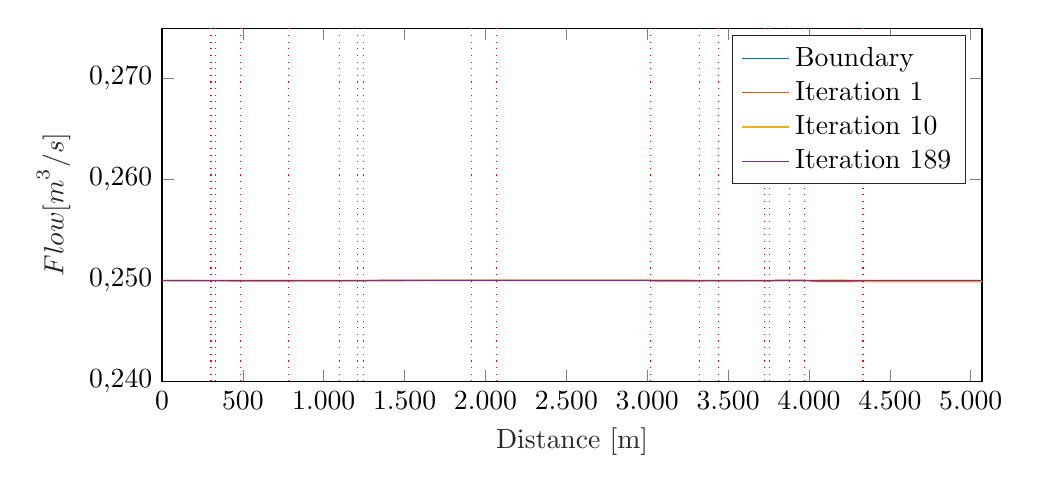
\begin{tikzpicture}

% \begin{axis}[%
% width=5.1in,
% height=2.661in,
% at={(2.08in,4.154in)},
% scale only axis,
% xmin=0,
% xmax=5070,
% xlabel style={font=\color{white!15!black}},
% xlabel={Distance [m]},
% ymin=0.23,
% ymax=0.5,
% ylabel style={font=\color{white!15!black}},
% ylabel={Height [m]},
% y tick label style={
%         /pgf/number format/.cd,
%             fixed,
%             fixed zerofill,
%             precision=3,
%         /tikz/.cd  },
% axis background/.style={fill=white},
% title style={font=\bfseries},
% title={Lookup table},
% legend style={legend cell align=left, align=left, draw=white!15!black}
% ]
% \addplot [color=mycolor1]
%   table[row sep=crcr]{%
% 0	0.349019999999655\\
% 303	0.349019999999655\\
% 303	0.337400000000343\\
% 330	0.337400000000343\\
% 330	0.3121000000001\\
% 485	0.3121000000001\\
% 485	0.255040000000008\\
% 780	0.255040000000008\\
% 780	0.30257999999958\\
% 1098	0.30257999999958\\
% 1098	0.33335999999963\\
% 1208	0.33335999999963\\
% 1208	0.356700000000274\\
% 1246	0.356700000000274\\
% 1246	0.337400000000343\\
% 1911	0.337400000000343\\
% 1911	0.472200000000157\\
% 2066	0.472200000000157\\
% 2066	0.321600000000217\\
% 3021	0.321600000000217\\
% 3021	0.318839999999909\\
% 3325	0.318839999999909\\
% 3325	0.348359999999957\\
% 3441	0.348359999999957\\
% 3441	0.350139999999556\\
% 3724	0.350139999999556\\
% 3724	0.340619999999944\\
% 3755	0.340619999999944\\
% 3755	0.319040000000314\\
% 3880	0.319040000000314\\
% 3880	0.366450000000441\\
% 3974	0.366450000000441\\
% 3974	0.262560000000121\\
% 4334	0.262560000000121\\
% 4334	0.366399999999885\\
% 5070	0.366399999999885\\
% };
% \addlegendentry{Boundary}

% \addplot [color=mycolor2]
%   table[row sep=crcr]{%
% 0	0.349019999999655\\
% 80.8000000000002	0.349020481316074\\
% 303	0.349020000000564\\
% 303	0.337400000000343\\
% 330	0.337380589420718\\
% 330	0.3121000000001\\
% 368.75	0.312106867829243\\
% 485	0.312100028022542\\
% 485	0.255040000000008\\
% 611.428571428572	0.255040284774623\\
% 780	0.255040001183261\\
% 780	0.30257999999958\\
% 843.6	0.302577760769054\\
% 1098	0.302579999983209\\
% 1098	0.33335999999963\\
% 1186	0.333359622993157\\
% 1208	0.333359874085545\\
% 1208	0.356700000000274\\
% 1246	0.356708069378328\\
% 1246	0.337400000000343\\
% 1268.16666666667	0.337368396814782\\
% 1334.66666666667	0.337399179543354\\
% 1911	0.337400000000343\\
% 1911	0.472200000000157\\
% 2066	0.472199999998338\\
% 2066	0.321600000000217\\
% 2257	0.321599999286263\\
% 3021	0.321600000000217\\
% 3021	0.318959999999606\\
% 3041.26666666667	0.318844345599246\\
% 3325	0.318840000006276\\
% 3325	0.348359999999957\\
% 3371.4	0.348355689153323\\
% 3441	0.348359969182638\\
% 3441	0.350139999999556\\
% 3511.75	0.350140224120878\\
% 3724	0.350140000011379\\
% 3724	0.340619999999944\\
% 3755	0.340622273461122\\
% 3755	0.319040000000314\\
% 3775.83333333333	0.319007018123557\\
% 3817.5	0.319038499465933\\
% 3880	0.319039982874529\\
% 3880	0.366450000000441\\
% 3974	0.366450006908963\\
% 3974	0.262560000000121\\
% 3998	0.262606505555596\\
% 4046	0.262563473184855\\
% 4334	0.262560000153826\\
% 4334	0.366399999999885\\
% 4530.26666666667	0.366399999871646\\
% 5070	0.366399999999885\\
% };
% \addlegendentry{Iterration 1}

% \addplot [color=mycolor3]
%   table[row sep=crcr]{%
% 0	0.349019999999655\\
% 60.6000000000004	0.349036522010465\\
% 303	0.349029645651171\\
% 303	0.337400000000343\\
% 330	0.337375436085495\\
% 330	0.3121000000001\\
% 388.125	0.312116053602949\\
% 485	0.312113124059579\\
% 485	0.255040000000008\\
% 548.214285714286	0.255059158875156\\
% 780	0.255055547565462\\
% 780	0.30257999999958\\
% 1098	0.302564515821359\\
% 1098	0.33335999999963\\
% 1142	0.333332646147028\\
% 1208	0.333340608369326\\
% 1208	0.356700000000274\\
% 1246	0.356718336754966\\
% 1246	0.337400000000343\\
% 1290.33333333333	0.337362335213584\\
% 1911	0.337399999565605\\
% 1911	0.472200000000157\\
% 2043.85714285714	0.472192406379691\\
% 2066	0.472192812377216\\
% 2066	0.321600000000217\\
% 2161.5	0.321588994348531\\
% 3021	0.321600000000217\\
% 3021	0.318959999999606\\
% 3041.26666666667	0.318909314883058\\
% 3304.73333333333	0.318869159727001\\
% 3325	0.318859556761709\\
% 3325	0.348359999999957\\
% 3394.6	0.348327480761327\\
% 3441	0.348324021764711\\
% 3441	0.350139999999556\\
% 3511.75	0.350125604256391\\
% 3724	0.350143100147761\\
% 3724	0.340619999999944\\
% 3755	0.340626457929829\\
% 3755	0.319040000000314\\
% 3775.83333333333	0.318989076884463\\
% 3880	0.318987695751275\\
% 3880	0.366450000000441\\
% 3903.5	0.366394930784736\\
% 3974	0.366409957899123\\
% 3974	0.262560000000121\\
% 4022	0.262614928369658\\
% 4214	0.262630593074391\\
% 4334	0.262577626555867\\
% 4334	0.366399999999885\\
% 4432.13333333333	0.36639104866299\\
% 5070	0.366399999999885\\
% };
% \addlegendentry{Iteration 10}

% \addplot [color=mycolor4]
%   table[row sep=crcr]{%
% 0	0.349019999999655\\
% 60.6000000000004	0.349036522010465\\
% 303	0.349036522123242\\
% 303	0.337400000000343\\
% 330	0.337383528097234\\
% 330	0.3121000000001\\
% 368.75	0.312127255888299\\
% 485	0.312127255888299\\
% 485	0.255040000000008\\
% 527.142857142857	0.255070957815406\\
% 780	0.25507095868943\\
% 780	0.30257999999958\\
% 843.6	0.302597889077333\\
% 1098	0.302597889182834\\
% 1098	0.33335999999963\\
% 1208	0.333365460569439\\
% 1208	0.356700000000274\\
% 1246	0.356742349043088\\
% 1246	0.337400000000343\\
% 1312.5	0.337383528097234\\
% 1911	0.337383528097234\\
% 1911	0.472200000000157\\
% 1955.28571428571	0.472168027992666\\
% 2066	0.472168027992666\\
% 2066	0.321600000000217\\
% 2113.75	0.321570504886949\\
% 3021	0.321570503379917\\
% 3021	0.318839999999909\\
% 3061.53333333333	0.318880063972756\\
% 3325	0.318880065802659\\
% 3325	0.348359999999957\\
% 3441	0.348367034051989\\
% 3441	0.350139999999556\\
% 3488.16666666667	0.350168559149097\\
% 3724	0.350168562385988\\
% 3724	0.340619999999944\\
% 3755	0.340652255206805\\
% 3755	0.319040000000314\\
% 3796.66666666667	0.319013727231322\\
% 3880	0.319013719325085\\
% 3880	0.366450000000441\\
% 3927	0.366424689039377\\
% 3974	0.366424681146782\\
% 3974	0.262560000000121\\
% 3998	0.262614845033568\\
% 4334	0.26261485766554\\
% 4334	0.366399999999885\\
% 4358.53333333333	0.366466726264662\\
% 5070	0.366466605791175\\
% };
% \addlegendentry{Iteration 189}

% \addplot [color=red, dotted, forget plot]
%   table[row sep=crcr]{%
% 303	0.230000000000018\\
% 303	0.5\\
% };
% \addplot [color=red, dotted, forget plot]
%   table[row sep=crcr]{%
% 330	0.230000000000018\\
% 330	0.5\\
% };
% \addplot [color=red, dotted, forget plot]
%   table[row sep=crcr]{%
% 485	0.230000000000018\\
% 485	0.5\\
% };
% \addplot [color=red, dotted, forget plot]
%   table[row sep=crcr]{%
% 780	0.230000000000018\\
% 780	0.5\\
% };
% \addplot [color=red, dotted, forget plot]
%   table[row sep=crcr]{%
% 1098	0.230000000000018\\
% 1098	0.5\\
% };
% \addplot [color=red, dotted, forget plot]
%   table[row sep=crcr]{%
% 1208	0.230000000000018\\
% 1208	0.5\\
% };
% \addplot [color=red, dotted, forget plot]
%   table[row sep=crcr]{%
% 1246	0.230000000000018\\
% 1246	0.5\\
% };
% \addplot [color=red, dotted, forget plot]
%   table[row sep=crcr]{%
% 1911	0.230000000000018\\
% 1911	0.5\\
% };
% \addplot [color=red, dotted, forget plot]
%   table[row sep=crcr]{%
% 2066	0.230000000000018\\
% 2066	0.5\\
% };
% \addplot [color=red, dotted, forget plot]
%   table[row sep=crcr]{%
% 3021	0.230000000000018\\
% 3021	0.5\\
% };
% \addplot [color=red, dotted, forget plot]
%   table[row sep=crcr]{%
% 3325	0.230000000000018\\
% 3325	0.5\\
% };
% \addplot [color=red, dotted, forget plot]
%   table[row sep=crcr]{%
% 3441	0.230000000000018\\
% 3441	0.5\\
% };
% \addplot [color=red, dotted, forget plot]
%   table[row sep=crcr]{%
% 3724	0.230000000000018\\
% 3724	0.5\\
% };
% \addplot [color=red, dotted, forget plot]
%   table[row sep=crcr]{%
% 3755	0.230000000000018\\
% 3755	0.5\\
% };
% \addplot [color=red, dotted, forget plot]
%   table[row sep=crcr]{%
% 3880	0.230000000000018\\
% 3880	0.5\\
% };
% \addplot [color=red, dotted, forget plot]
%   table[row sep=crcr]{%
% 3974	0.230000000000018\\
% 3974	0.5\\
% };
% \addplot [color=red, dotted, forget plot]
%   table[row sep=crcr]{%
% 4334	0.229999999999563\\
% 4334	0.5\\
% };
% \end{axis}

\begin{axis}[%
/pgf/number format/1000 sep={.},/pgf/number format/use comma,
width=4.1in,
height=1.7661in,
at={(2.08in,0.858in)},
scale only axis,
xmin=0,
xmax=5070,
xlabel style={font=\color{white!15!black}},
xlabel={Distance [m]},
ymin=0.24,
ymax=0.275,
ylabel style={font=\color{white!15!black}},
ylabel={$\text{Flow [m}^\text{3}\text{/s]}$},
y tick label style={
        /pgf/number format/.cd,
            fixed,
            fixed zerofill,
            precision=3,
        /tikz/.cd  },
axis background/.style={fill=white},
legend style={legend cell align=left, align=left, draw=white!15!black}
]
\addplot [color=mycolor1]
  table[row sep=crcr]{%
0	0.25\\
303	0.25\\
330	0.25\\
485	0.25\\
780	0.25\\
1098	0.25\\
1208	0.25\\
1246	0.25\\
1911	0.25\\
2066	0.25\\
3021	0.25\\
3325	0.25\\
3441	0.25\\
3724	0.25\\
3755	0.25\\
3880	0.25\\
3974	0.25\\
4334	0.25\\
5070	0.25\\
};
\addlegendentry{Boundary}

\addplot [color=mycolor2]
  table[row sep=crcr]{%
0	0.25\\
60.6000000000004	0.249978522559104\\
181.8	0.249976578495989\\
303	0.249976576241352\\
330	0.249995637611391\\
388.125	0.249960527929943\\
446.25	0.249956389295221\\
485	0.249956152021696\\
590.357142857143	0.249940082209832\\
780	0.249939045288556\\
843.6	0.24996667841333\\
928.400000000001	0.249970279605805\\
1098	0.249970385933921\\
1164	0.249990196854014\\
1208	0.249991662936736\\
1246	0.249952059458337\\
1268.16666666667	0.249977538387611\\
1290.33333333333	0.25001056144356\\
1312.5	0.25002033943565\\
1379	0.250024345979909\\
1911	0.250024452777325\\
1977.42857142857	0.250032223487324\\
2066	0.250032254260077\\
2137.625	0.250045787679483\\
2543.5	0.25004626554346\\
3021	0.25004626554346\\
3041.26666666667	0.249943509264085\\
3081.8	0.24993731453651\\
3325	0.249936628178148\\
3371.4	0.24998358783705\\
3417.8	0.249989579559042\\
3441	0.249989769594322\\
3488.16666666667	0.249961217600685\\
3582.5	0.249958852517011\\
3724	0.249958843491186\\
3755	0.249955586868964\\
3775.83333333333	0.249989375663972\\
3796.66666666667	0.250030383417652\\
3817.5	0.250039139651562\\
3880	0.250041486897317\\
3974	0.250034890455026\\
3998	0.249984011331435\\
4022	0.249919238147413\\
4046	0.24990154439547\\
4094	0.249895386285061\\
4334	0.249894859729466\\
4407.6	0.249908068946752\\
5070	0.249908105777649\\
};
\addlegendentry{Iteration 1}

\addplot [color=mycolor3]
  table[row sep=crcr]{%
0	0.25\\
262.6	0.249996705091689\\
303	0.249990246794368\\
330	0.249987987705936\\
485	0.249977241522174\\
780	0.249969651238644\\
864.8	0.249959840581141\\
1034.4	0.249941208218843\\
1098	0.249944758969832\\
1164	0.249955518235765\\
1208	0.249962931765367\\
1246	0.249966418070471\\
1401.16666666667	0.249976220261487\\
1467.66666666667	0.249981009654221\\
1512	0.249984605378813\\
1667.16666666667	0.250021862440917\\
1822.33333333333	0.250024434770239\\
1911	0.250024452131584\\
2066	0.250025003068004\\
2304.75	0.250033845017242\\
2495.75	0.250046057881264\\
3021	0.25004626554346\\
3223.66666666667	0.250044100288505\\
3243.93333333333	0.250034984778722\\
3325	0.24996756830933\\
3441	0.249937825736197\\
3535.33333333333	0.249941782698443\\
3582.5	0.249961131167765\\
3629.66666666667	0.249978221881975\\
3676.83333333333	0.249973853478878\\
3724	0.249963325268254\\
3755	0.249961808230182\\
3880	0.249958886077366\\
3927	0.249960381648634\\
3950.5	0.249966168777974\\
3974	0.249979746679855\\
3998	0.249986417225045\\
4070	0.250023586625503\\
4118	0.250034725949263\\
4190	0.250035535980714\\
4214	0.250030181091461\\
4238	0.250016839358977\\
4286	0.249970979716636\\
4334	0.249928669712972\\
4407.6	0.24989800178264\\
4481.2	0.249895426942203\\
4800.13333333333	0.249908105894974\\
5070	0.249908105777649\\
};
\addlegendentry{Iteration 10}

\addplot [color=mycolor4]
  table[row sep=crcr]{%
0	0.25\\
303	0.25\\
330	0.25\\
485	0.25\\
780	0.25\\
1098	0.25\\
1208	0.25\\
1246	0.25\\
1911	0.25\\
2066	0.25\\
3021	0.25\\
3325	0.25\\
3441	0.25\\
3724	0.25\\
3755	0.25\\
3880	0.25\\
3974	0.25\\
4334	0.25\\
5070	0.249999787922206\\
};
\addlegendentry{Iteration 189}

\addplot [color=red, dotted, forget plot]
  table[row sep=crcr]{%
303	0.240000000000009\\
303	0.274999999999977\\
};
\addplot [color=red, dotted, forget plot]
  table[row sep=crcr]{%
330	0.240000000000009\\
330	0.274999999999977\\
};
\addplot [color=red, dotted, forget plot]
  table[row sep=crcr]{%
485	0.240000000000009\\
485	0.274999999999977\\
};
\addplot [color=red, dotted, forget plot]
  table[row sep=crcr]{%
780	0.240000000000009\\
780	0.274999999999977\\
};
\addplot [color=red, dotted, forget plot]
  table[row sep=crcr]{%
1098	0.240000000000009\\
1098	0.275000000000091\\
};
\addplot [color=red, dotted, forget plot]
  table[row sep=crcr]{%
1208	0.240000000000009\\
1208	0.275000000000091\\
};
\addplot [color=red, dotted, forget plot]
  table[row sep=crcr]{%
1246	0.240000000000009\\
1246	0.275000000000091\\
};
\addplot [color=red, dotted, forget plot]
  table[row sep=crcr]{%
1911	0.240000000000009\\
1911	0.275000000000091\\
};
\addplot [color=red, dotted, forget plot]
  table[row sep=crcr]{%
2066	0.239999999999782\\
2066	0.275000000000091\\
};
\addplot [color=red, dotted, forget plot]
  table[row sep=crcr]{%
3021	0.239999999999782\\
3021	0.275000000000091\\
};
\addplot [color=red, dotted, forget plot]
  table[row sep=crcr]{%
3325	0.239999999999782\\
3325	0.275000000000091\\
};
\addplot [color=red, dotted, forget plot]
  table[row sep=crcr]{%
3441	0.239999999999782\\
3441	0.275000000000091\\
};
\addplot [color=red, dotted, forget plot]
  table[row sep=crcr]{%
3724	0.239999999999782\\
3724	0.275000000000091\\
};
\addplot [color=red, dotted, forget plot]
  table[row sep=crcr]{%
3755	0.239999999999782\\
3755	0.275000000000091\\
};
\addplot [color=red, dotted, forget plot]
  table[row sep=crcr]{%
3880	0.239999999999782\\
3880	0.275000000000091\\
};
\addplot [color=red, dotted, forget plot]
  table[row sep=crcr]{%
3974	0.239999999999782\\
3974	0.275000000000091\\
};
\addplot [color=red, dotted, forget plot]
  table[row sep=crcr]{%
4334	0.239999999999782\\
4334	0.274999999999636\\
};
\end{axis}
\end{tikzpicture}%
% %\caption{Height and flow of pipe setup from part of Fredericia where boundary conditions is found by lookup table. Various amount of iterations, with constant flow input of 0,25 $\text{m}^\text{3}$/s, is performed. The dotted line indicates pipe intersections.}
% \label{fig:fredericia_init_steady_state_lut}
% \end{figure}  
%  \vfill\vfill
% \end{frame}

%\subsection{Simulering}

\begin{frame}{Implementering}{Simulering}
\vfill \vfill \centering
    \begin{itemize}
    	\item Beregner parameter for hvert tidsskridt 
    \end{itemize}

    \begin{figure}[H]
\centering
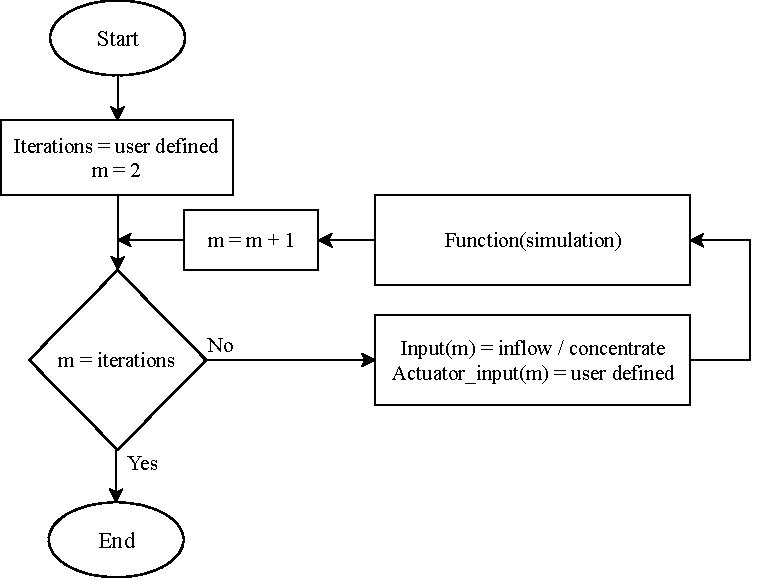
\includegraphics[width=0.5 \textwidth]{figures/simu_main_chart.pdf}
%\caption{Main Simulering loop.}
\label{fig:simu_main_chart}
\end{figure}

%\subsection{Display}
\vfill \vfill
\end{frame}

\begin{frame}{Implementering}{Display}
     \begin{figure}[h]
 \centering
 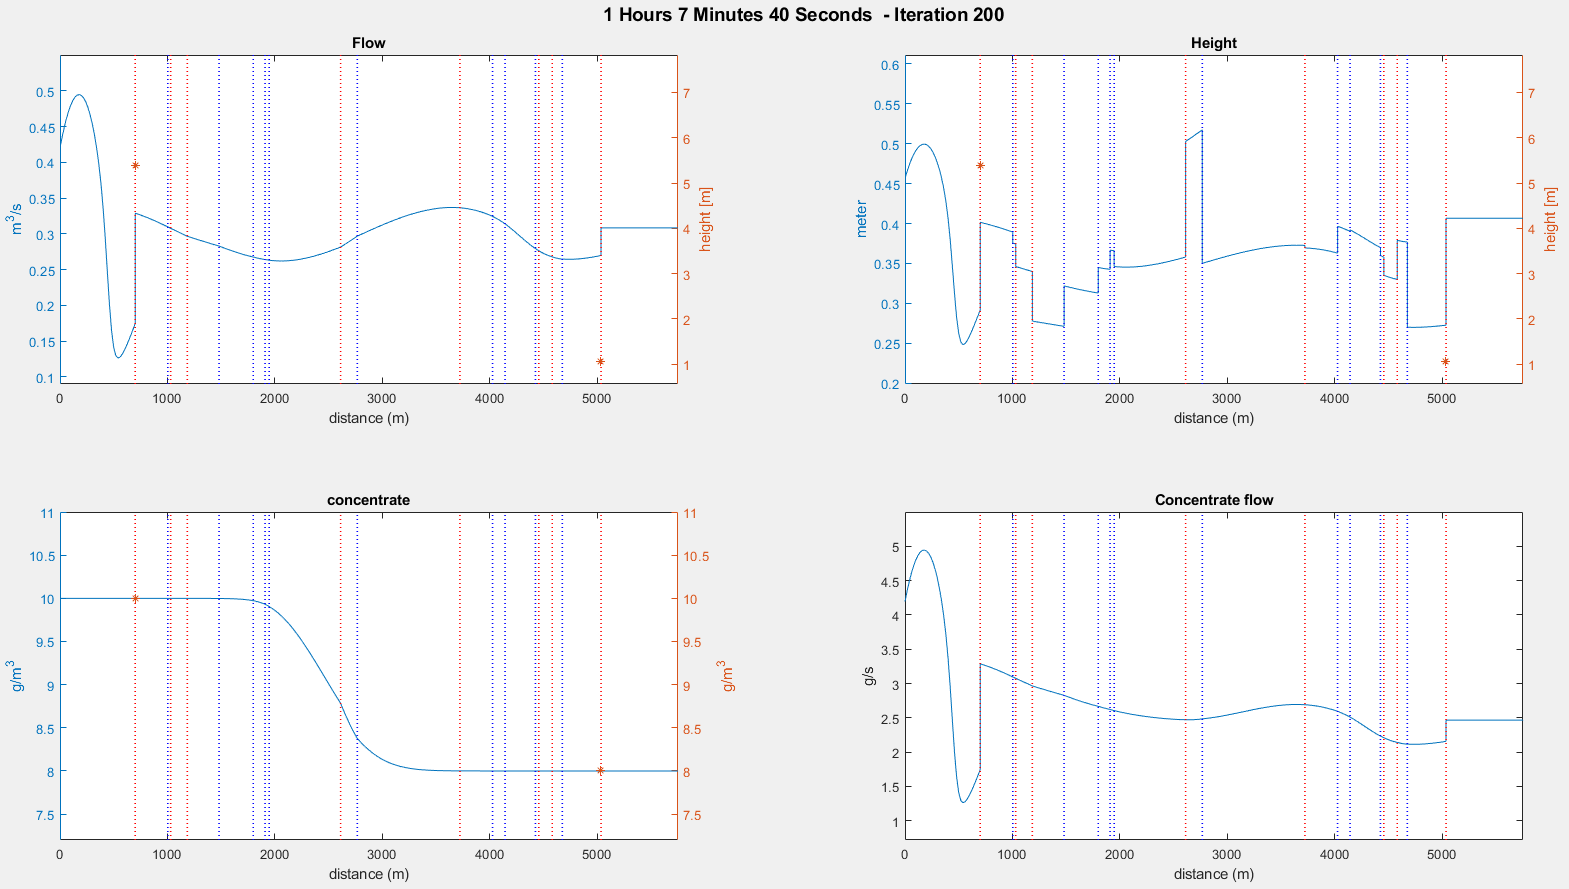
\includegraphics[width=1.0 \textwidth]{figures/display_result_matlab.png}
 %\caption
 \label{fig:display_result_matlab}
 \end{figure}
\end{frame}


\section{Kontrol}
\subsection{Linearisering}
\begin{frame}{Kontrol}{Linearisering}
 \vfill\vfill\centering    
\begin{itemize}
	\item Lineær model til MPC\vspace{5mm}
	\item Kontinuitets ligningen \vspace{5mm}
	\item Højde states \vspace{5mm}
	\item Preissmann scheme \vspace{5mm}
\end{itemize}
\begin{equation*}\label{eq:linearization_Continuity}
\frac{\partial A(x,t)}{\partial t} + \frac{\partial Q(x,t)}{\partial x}=0
\end{equation*}\vspace{5mm}
\begin{equation*}
	\frac{\partial A(h)}{\partial h}\frac{\partial h(x,t)}{\partial t} + \frac{\partial Q(h)}{\partial h}\frac{\partial h(x,t)}{\partial x}=0
\end{equation*}
\vfill\vfill
\end{frame}

\begin{frame}{Kontrol}{Opsætning af state space}
 \vfill\vfill\centering    
\begin{itemize}
%	\item Opsat på matrix og vektor form \vspace{5mm}
	\item Opstilles på state space form   \vspace{5mm}
\end{itemize}
\begin{equation*}\label{eq:rearrange_continuity_eq}
\begin{aligned}
	&\begin{bmatrix}
		\underbrace{\frac{1}{2\Delta t}\frac{\partial A}{\partial h}-\frac{\theta}{\Delta x}\frac{\partial Q}{\partial h}}_{a} & \underbrace{\frac{1}{2\Delta t}\frac{\partial A}{\partial h}+\frac{\theta}{\Delta x}\frac{\partial Q}{\partial h}}_{b} 
	\end{bmatrix}
	\begin{bmatrix}
		h_{j}^{i+1} \\
		h_{j+1}^{i+1}
	\end{bmatrix}
	= \\ \vspace{5mm} -
	&\begin{bmatrix}
		\underbrace{\frac{-1}{2\Delta t}\frac{\partial A}{\partial h}-\frac{(1-\theta)}{\Delta x}\frac{\partial Q}{\partial h}}_{c} & \underbrace{\frac{-1}{2\Delta t}\frac{\partial A}{\partial h}+\frac{(1-\theta)}{\Delta x}\frac{\partial Q}{\partial h}}_{d} 
	\end{bmatrix}
	\begin{bmatrix}
		h_{j}^{i} \\
		h_{j+1}^{i}
	\end{bmatrix}
	\end{aligned}
\end{equation*}
\vfill\vfill
\end{frame}




\begin{frame}{Kontrol}{Opsætning på state space}
\vfill \vfill \centering
 \begin{equation*}
\begin{aligned}
	   \underbrace{\begin{bmatrix}
	    	1 & 0    & 0    &\cdots &0\\
	    	0 & b_1  & 0    &\cdots &0\\
	    	0 &a_{1} & b_2  &\ddots &\vdots	  \\
	    \vdots&\vdots&\ddots&\ddots & 0  \\
	        0 & 0    &0  	&a_{m-1}&  b_m\\
	   \end{bmatrix}}_{\xi}
	    \underbrace{\begin{bmatrix}
		h_{0}^{i+1}\\
		h_{1}^{i+1} \\
		h_{2}^{i+1} \\			
		\vdots		\\
		h_{m}^{i+1}\\
	\end{bmatrix}}_{x(k+1)}
	=& 
	\underbrace{\begin{bmatrix}
	    	0 &  0   &   0    & \cdots   &0\\
	    c_{0} & d_1  &   0    &  \cdots  &0\\
	    0	  &c_{1} & d_2    & \cdots   &0 \\
	    \vdots&\vdots&\ddots  & \ddots   & \vdots\\
	    0	  & 0    &  0     &  c_{m-1} &  d_m\\
	    \end{bmatrix}}_{A}
	    	\underbrace{\begin{bmatrix}
		h_{0}^{i} \\
		h_{1}^{i} \\
		h_{2}^{i}\\
		\vdots		\\
		h_{m}^{i}\\
		\end{bmatrix}}_{x(k)}
	+ \\ \vspace{5mm} & \underbrace{\begin{bmatrix}
		 1\\
		 -a_0 \\
		 0\\
		 \vdots \\
		 0\\
		\end{bmatrix}}_{B}
		h_0^{i+1}
		% \underbrace{\begin{bmatrix}
		% h_{0}^{i} \\
		% h_{0}^{i+1} \\
		% \end{bmatrix}}_{u}
		+ 
		\underbrace{\begin{bmatrix}
		 \frac{dh}{dQ}\\
		 0 \\
		 0\\
		 \vdots \\
		 0\\
		\end{bmatrix}}_{B_d}
		d_{0}^{i+1}
	\end{aligned}
\end{equation*}   
\vfill \vfill
\end{frame}

\begin{frame}{Kontrol}{Indsætning af tank}
\vfill \vfill \centering
\begin{itemize}
	\item e - Forøgelse af højde i tank(inflow)
	\item f - Reducering af højde i tank(Outflow)
	\item g - Inflow i efterfølgende rør
\end{itemize}
\begin{equation*}\label{eq:tank_linear_implement_ss}
\begin{aligned}
      & \underbrace{\begin{bmatrix}
%            1 & 0       & 0         &0          &0          &0   &0\\
%            0 & b_{1,1} & 0         &0          &0          &0  &0\\
            %0 &a_{1,1}  & 
            b_{1,2}   & 0         &0          &0 \\ %0\\
          %  0 &0        & 
            0         & 1         & 0         &0     \\ % &0\\
          %   0 &0        & \\ 
             0         &  0        & 1         &0  \\ % & 0        \\
           % 0 & 0       &
            0          &  0         &a_{2,1}    &  b_{2,2}\\ %&0       \\
%            0 & 0       & 0         &   0        &     0      & a_{2,2}  & b_{2,3}\\  
       \end{bmatrix}}_{\xi}
        \underbrace{\begin{bmatrix}
%        h_{1,0}^{i+1}\\
 %       h_{1,1}^{i+1} \\
        h_{1,2}^{i+1} \\ 
        h_{tank}^{i+1} \\          
        h_{2,0}^{i+1}     \\
        h_{2,1}^{i+1}\\
  %      h_{2,2}^{i+1}\\
    \end{bmatrix}}_{x(k+1)}
    \\ &=
    \underbrace{\begin{bmatrix}
 %       0       &  0    &   0    & 0     &0         &0          &0 \\
  %      c_{1,0} &d_{1,1}&   0    &  0    &0         &0          &0\\
        %0       &c_{1,1}&
         d_{1,2}& 0     &0         &0 \\ %      &0\\
       % 0       & 0     & 
       e    & 1     &0         &0     \\ %     &0           \\
        %0       & 0     & 
          0    & 0     & 0        &0       \\ %   &0        \\
        %0       & 0     & 
         0     & 0    &c_{2,0}    &  d_{2,1} \\ %&0  \\
   %      0       & 0     &  0    & 0    &0          &c_{2,1}    &  d_{2,2}   \\
        \end{bmatrix}}_{A}
            \underbrace{\begin{bmatrix}
  %      h_{1,0}^{i} \\
   %     h_{1,1}^{i} \\
        h_{1,2}^{i} \\
        h_{tank}^{i}\\
        h_{2,0}^{i}\\
        h_{2,1}^{i}\\
    %      h_{2,2}^{i}\\
        \end{bmatrix}}_{x(k)}
    +  \underbrace{\begin{bmatrix}
   %      1 & 0\\
    %     -a_0& 0 \\
         0 & 0\\
          0& -f \\
          0& g \\ 
          0& 0 \\
     %     0& 0 \\
        \end{bmatrix}}_{B}
        \begin{bmatrix}
        h_0^{i+1}\\
        u_{tank} \\
        \end{bmatrix}
    \end{aligned}
\end{equation*}    
\vfill \vfill
\end{frame}

\begin{frame}{Kontrol}{Test}
   \vfill\vfill\centering
    \begin{minipage}[t]{0.48\linewidth}
\begin{itemize}
		\item Samligning af ulineær og lineær model for små forstyrrelser
		\item System setup
	   	\item Sinus input
\end{itemize}    
\end{minipage}\hfill
\begin{minipage}[t]{0.48\linewidth}
\begin{table}[H]
\centering
\begin{tabular}{|c|c|c|}
\hline
	\rowcolor[HTML]{9B9B9B} 
Type  & Components & Sections \\ \hline
Pipe  & 1         & 35       \\ \hline
Tank  & 1         & 1        \\ \hline
Pipe  & 18        & 227      \\ \hline
Total & 20        & 263      \\ \hline
\end{tabular}
%\caption{System setup.}
\label{tab:system_setup_nonlinear_linear_test}
\end{table}

\end{minipage}
\vfill\vfill

\end{frame}

\begin{frame}{Kontrol}{Test}
\vfill \vfill \centering
% \begin{figure}
% \centering
% % This file was created by matlab2tikz.
%
%The latest updates can be retrieved from
%  http://www.mathworks.com/matlabcentral/fileexchange/22022-matlab2tikz-matlab2tikz
%where you can also make suggestions and rate matlab2tikz.
%
\definecolor{mycolor1}{rgb}{0.00000,0.44700,0.74100}%
%
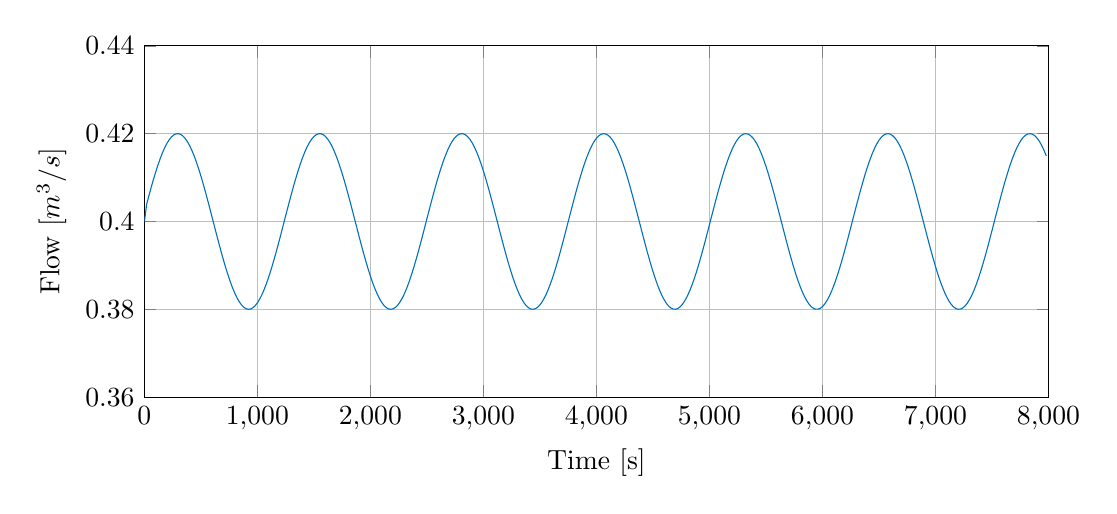
\begin{tikzpicture}

\begin{axis}[%
width=4.521in,
height=1.7566in,
at={(0.758in,0.481in)},
scale only axis,
xmin=0,
xmajorgrids,
ymajorgrids,
xmax=8000,
ymin=0.36,
ymax=0.44,
xlabel={Time [s]},
ylabel={Flow $[m^3/s]$},
axis background/.style={fill=white}
]
\addplot [color=mycolor1,solid,forget plot]
  table[row sep=crcr]{%
1	0.4\\
21	0.403973386615901\\
41	0.405910404133227\\
61	0.407788366846173\\
81	0.409588510772084\\
101	0.411292849467901\\
121	0.412884353744754\\
141	0.41434712181799\\
161	0.41566653819255\\
181	0.416829419696158\\
201	0.417824147201229\\
221	0.418640781719345\\
241	0.419271163708344\\
261	0.419708994599769\\
281	0.419949899732081\\
301	0.41999147206083\\
321	0.419833296209049\\
341	0.419476952617564\\
361	0.418926001753748\\
381	0.418185948536514\\
401	0.417264187332977\\
421	0.416169928076392\\
441	0.414914104243534\\
461	0.413509263611023\\
481	0.411969442882079\\
501	0.410310027436429\\
521	0.408547597604677\\
541	0.406699763003118\\
561	0.40478498658428\\
581	0.402822400161197\\
601	0.400831613248666\\
621	0.398832517131448\\
641	0.396845086117135\\
661	0.394889177959463\\
681	0.392984335446208\\
701	0.391149591134103\\
721	0.38940327718183\\
741	0.387762842181146\\
761	0.386244676816321\\
781	0.384863950093841\\
801	0.383634457778712\\
821	0.382568484551728\\
841	0.381676681265011\\
861	0.38096795852221\\
881	0.380449397646698\\
901	0.380126179927331\\
921	0.380001534848718\\
941	0.380076707823283\\
961	0.380350947747513\\
981	0.380821514506737\\
1001	0.381483706353445\\
1021	0.382330906885597\\
1041	0.383354651155522\\
1061	0.38454471024888\\
1081	0.385889193488592\\
1101	0.387374667242554\\
1121	0.388986289148047\\
1141	0.390707956411725\\
1161	0.392522466703395\\
1181	0.394411690036022\\
1201	0.396356749914558\\
1221	0.39833821194365\\
1241	0.400336278009687\\
1261	0.40233098409701\\
1281	0.404302399761756\\
1301	0.406230827270268\\
1321	0.408096998412332\\
1341	0.409882267022772\\
1361	0.411568795287764\\
1381	0.413139731974376\\
1401	0.414579380802518\\
1421	0.415873357276983\\
1441	0.417008732412571\\
1461	0.417974161916233\\
1481	0.418759999535495\\
1501	0.41935839344063\\
1521	0.41976336467754\\
1541	0.419970866907492\\
1561	0.419978826836795\\
1581	0.419787164932468\\
1601	0.419397796216902\\
1621	0.418814611133595\\
1641	0.418043436675126\\
1661	0.417091978161766\\
1681	0.41596974225247\\
1701	0.414687941957482\\
1721	0.413259384601644\\
1741	0.411698343857835\\
1761	0.410020417129158\\
1781	0.408242369704835\\
1801	0.406381967246987\\
1821	0.404457798282005\\
1841	0.402489088470141\\
1861	0.400495508509067\\
1881	0.398496977590764\\
1901	0.39651346437554\\
1921	0.394564787471781\\
1941	0.392670417414961\\
1961	0.390849282124494\\
1981	0.389119577782213\\
2001	0.387498587022142\\
2021	0.386002506248129\\
2041	0.384646283804728\\
2061	0.383443470618287\\
2081	0.382406084800567\\
2101	0.381544491567744\\
2121	0.380867299674596\\
2141	0.38038127539867\\
2161	0.380091274933872\\
2181	0.380000195868986\\
2201	0.38010894823592\\
2221	0.380416445416974\\
2241	0.380919615001958\\
2261	0.381613429486707\\
2281	0.382490956506231\\
2301	0.383543428100626\\
2321	0.384760328321619\\
2341	0.386129498304458\\
2361	0.387637257755259\\
2381	0.389268541639991\\
2401	0.391007050709308\\
2421	0.392835414355263\\
2441	0.394735364172684\\
2461	0.396687916491034\\
2481	0.398673562052976\\
2501	0.400672460944423\\
2521	0.402664640828399\\
2541	0.404630196502031\\
2561	0.406549488782754\\
2581	0.408403340736533\\
2601	0.410173229287447\\
2621	0.411841470294144\\
2641	0.413391395243932\\
2661	0.414807517799049\\
2681	0.416075688531032\\
2701	0.41718323629713\\
2721	0.418119094846169\\
2741	0.418873913388882\\
2761	0.4194401500279\\
2781	0.419812147113897\\
2801	0.419986187774958\\
2821	0.419960533054327\\
2841	0.419735439285492\\
2861	0.419313155530986\\
2881	0.418697901110494\\
2901	0.41789582344281\\
2921	0.416914936622859\\
2941	0.415765041347506\\
2961	0.41445762699024\\
2981	0.413005756803142\\
3001	0.4114239373932\\
3021	0.409727973777076\\
3041	0.407934811462612\\
3061	0.406062367134914\\
3081	0.404129349638756\\
3101	0.402155073045989\\
3121	0.400159263675719\\
3141	0.398161862995446\\
3161	0.396182828372516\\
3181	0.394241933666699\\
3201	0.39235857165632\\
3221	0.390551560272031\\
3241	0.388838954574264\\
3261	0.387237866353041\\
3281	0.385764293152618\\
3301	0.384432958429314\\
3321	0.383257164439605\\
3341	0.38224865932837\\
3361	0.381417519745313\\
3381	0.380772050162409\\
3401	0.380318699898367\\
3421	0.380061998679168\\
3441	0.38000451137854\\
3461	0.380146812390587\\
3481	0.380487479890637\\
3501	0.381023110041638\\
3521	0.381748351004176\\
3541	0.382655956410288\\
3561	0.38373685776677\\
3581	0.384980255064567\\
3601	0.38637372468889\\
3621	0.387903343551874\\
3641	0.389553828207465\\
3661	0.391308687558562\\
3681	0.393150387630608\\
3701	0.395060526765268\\
3721	0.397020019483716\\
3741	0.399009287182433\\
3761	0.401008453756136\\
3781	0.402997544193259\\
3801	0.404956684159659\\
3821	0.406866298576398\\
3841	0.408707307207458\\
3861	0.410461315303154\\
3881	0.412110797394392\\
3901	0.413639272401363\\
3921	0.415031468307043\\
3941	0.416273474750142\\
3961	0.417352882012833\\
3981	0.418258905014553\\
4001	0.418982491072958\\
4021	0.41951641035534\\
4041	0.419855328116718\\
4061	0.419995858002853\\
4081	0.419936595885576\\
4101	0.419678133892372\\
4121	0.419223054490042\\
4141	0.418575904681545\\
4161	0.417743150573847\\
4181	0.416733112770721\\
4201	0.415555883236022\\
4221	0.41422322445812\\
4241	0.412748451923005\\
4261	0.411146301070353\\
4281	0.409432780061884\\
4301	0.407625009833099\\
4321	0.405741053026555\\
4341	0.403799733515909\\
4361	0.401820448323997\\
4381	0.399822973814192\\
4401	0.397827268091518\\
4421	0.395853271587865\\
4441	0.393920707823779\\
4461	0.392048886337571\\
4481	0.39025650975079\\
4501	0.388561486897809\\
4521	0.386980753886675\\
4541	0.385530104879115\\
4561	0.384224034280492\\
4581	0.383075591916497\\
4601	0.382096252643606\\
4621	0.381295801696109\\
4641	0.380682236915279\\
4661	0.380261688837587\\
4681	0.380038359440412\\
4701	0.380014480157267\\
4721	0.380190289582057\\
4741	0.380564031085123\\
4761	0.381131970364909\\
4781	0.381888432759868\\
4801	0.382825859947801\\
4821	0.383934885466121\\
4841	0.385204428298442\\
4861	0.38662180359244\\
4881	0.388172849402698\\
4901	0.389842068192188\\
4921	0.391612781678535\\
4941	0.393467297477906\\
4961	0.395387085881452\\
4981	0.397352964998045\\
5001	0.399345292413383\\
5021	0.40134416145051\\
5041	0.403329600070743\\
5061	0.405281770427689\\
5081	0.407181167080443\\
5101	0.409008811885508\\
5121	0.410746443620129\\
5141	0.412376700442401\\
5161	0.413883293365045\\
5181	0.415251169009592\\
5201	0.416466660014762\\
5221	0.417517621596218\\
5241	0.41839355289324\\
5261	0.419085701889854\\
5281	0.419587152862078\\
5301	0.419892895477557\\
5321	0.41999987485714\\
5341	0.419907022098231\\
5361	0.419615264954903\\
5381	0.41912751856809\\
5401	0.418448656338462\\
5421	0.417585461233014\\
5441	0.416546558011908\\
5461	0.415342327052711\\
5481	0.413984800633102\\
5501	0.412487542708328\\
5521	0.410865513384645\\
5541	0.409134919442884\\
5561	0.407313052405652\\
5581	0.405418115766157\\
5601	0.403469043104918\\
5621	0.401485308911687\\
5641	0.399486734002789\\
5661	0.397493287478071\\
5681	0.395524887196264\\
5701	0.393601200762316\\
5721	0.391741449015189\\
5741	0.389964213979589\\
5761	0.388287253200514\\
5781	0.386727322315741\\
5801	0.385300007639024\\
5821	0.384019570426808\\
5841	0.382898804384459\\
5861	0.381948907835796\\
5881	0.381179371833141\\
5901	0.380597885325856\\
5921	0.380210258334909\\
5941	0.380020363901061\\
5961	0.380030099386724\\
5981	0.380239367518143\\
6001	0.380646077357324\\
6021	0.381246165193994\\
6041	0.382033635148853\\
6061	0.383000619082413\\
6081	0.384137455210854\\
6101	0.385432784643368\\
6121	0.386873664876444\\
6141	0.388445699111085\\
6161	0.390133180100864\\
6181	0.391919247093539\\
6201	0.393786054298113\\
6221	0.395714949194082\\
6241	0.397686658901255\\
6261	0.399681482747998\\
6281	0.401679489113835\\
6301	0.403660714579612\\
6321	0.40560536339538\\
6341	0.407494005272989\\
6361	0.409307769527099\\
6381	0.411028533624834\\
6401	0.412639104260138\\
6421	0.414123389143607\\
6441	0.415466557791324\\
6461	0.416655189706156\\
6481	0.417677408470917\\
6501	0.418523000413611\\
6521	0.419183516659062\\
6541	0.419652357547283\\
6561	0.419924838575097\\
6581	0.419998237202145\\
6601	0.419871820053608\\
6621	0.419546850247845\\
6641	0.419026574775736\\
6661	0.418316192057816\\
6681	0.417422800003384\\
6701	0.416355325090529\\
6721	0.415124433175721\\
6741	0.413742422924095\\
6761	0.412223102925252\\
6781	0.410581653722401\\
6801	0.408834476133384\\
6821	0.406999027379133\\
6841	0.405093646656881\\
6861	0.403137371900968\\
6881	0.401149749562099\\
6901	0.399150639305661\\
6921	0.39716001558052\\
6941	0.395197768040925\\
6961	0.393283502815657\\
6981	0.391436346610077\\
7001	0.389674755598401\\
7021	0.388016331015715\\
7041	0.386477643292245\\
7061	0.385074066487102\\
7081	0.383819624675762\\
7101	0.382726851826141\\
7121	0.381806666563329\\
7141	0.381068263074301\\
7161	0.380519019242633\\
7181	0.380164422931138\\
7201	0.380008017148944\\
7221	0.380051364650927\\
7241	0.380294032323176\\
7261	0.380733595510525\\
7281	0.381365662242906\\
7301	0.382183917118463\\
7321	0.383180184404958\\
7341	0.384344509728987\\
7361	0.385665259536787\\
7381	0.38712923733286\\
7401	0.388721815534995\\
7421	0.390427081628232\\
7441	0.392227997157453\\
7461	0.394106567969995\\
7481	0.396044024007271\\
7501	0.398021006848994\\
7521	0.400017763136114\\
7541	0.40201434193985\\
7561	0.403990794104776\\
7581	0.405927371574188\\
7601	0.407804724706159\\
7621	0.409604095608765\\
7641	0.41130750556274\\
7661	0.412897934658897\\
7681	0.414359491855433\\
7701	0.415677573755966\\
7721	0.416839010521846\\
7741	0.417832197460829\\
7761	0.418647210977324\\
7781	0.419275907725682\\
7801	0.419712005975813\\
7821	0.419951148378156\\
7841	0.419990945500878\\
7861	0.419830999704283\\
7881	0.4194729091139\\
7901	0.418920251652538\\
7921	0.418178549290868\\
7941	0.417255212873714\\
7961	0.41615946807334\\
7981	0.414902263209587\\
};
\end{axis}
\end{tikzpicture}%
% %\caption{Comparison of the nonlinear and linear model at the last pipe in the setup.}
% \label{fig:linear_nonlinear_comparison__input_to_first_pipe}
% \end{figure}
\vspace{-5mm}
\begin{figure}
\centering
% This file was created by matlab2tikz.
%
%The latest updates can be retrieved from
%  http://www.mathworks.com/matlabcentral/fileexchange/22022-matlab2tikz-matlab2tikz
%where you can also make suggestions and rate matlab2tikz.
%
\definecolor{mycolor1}{rgb}{0.00000,0.44700,0.74100}%
\definecolor{mycolor2}{rgb}{0.85000,0.32500,0.09800}%
%
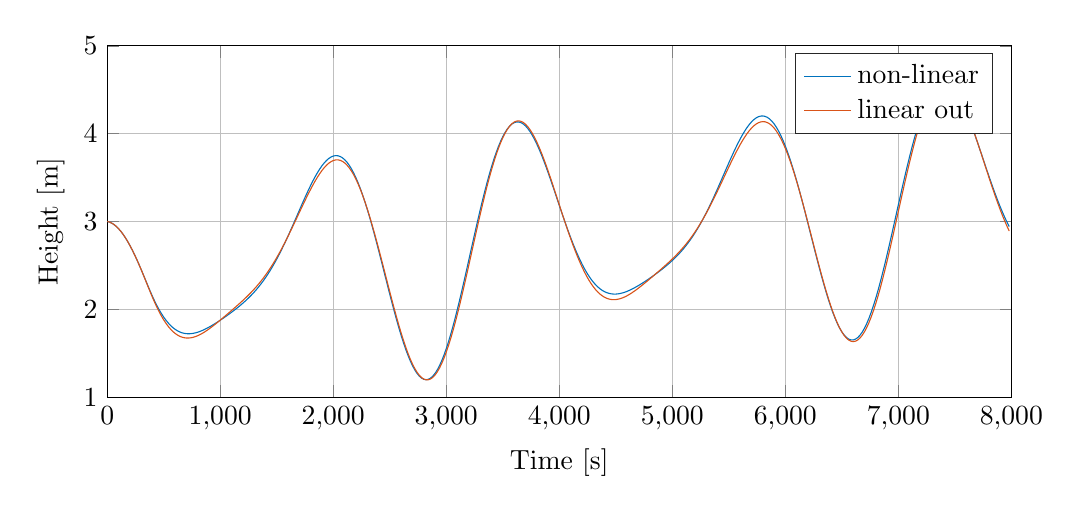
\begin{tikzpicture}

\begin{axis}[%
width=4.521in,
height=1.7566in,
at={(0.758in,0.481in)},
scale only axis,
xmin=0,
xmax=8000,
xlabel={Time [s]},
xmajorgrids,
ymin=1,
ymax=5,
ylabel={Height [m]},
ymajorgrids,
axis background/.style={fill=white},
legend style={legend cell align=left,align=left,draw=white!15!black}
]
\addplot [color=mycolor1,solid]
  table[row sep=crcr]{%
1	3\\
21	2.99281485388517\\
41	2.98089229877703\\
61	2.96429589132252\\
81	2.94311008270548\\
101	2.9174396709271\\
121	2.88740933874452\\
141	2.85316315177336\\
161	2.8148639575681\\
181	2.77269282398572\\
201	2.72684889042081\\
221	2.67755065665281\\
241	2.62504105449041\\
261	2.5696005464303\\
281	2.51157362705104\\
301	2.45141144588331\\
321	2.38972356923401\\
341	2.32731608105155\\
361	2.26518111636098\\
381	2.2044108927358\\
401	2.14604576423477\\
421	2.09091382444387\\
441	2.03953947939103\\
461	1.99216249068991\\
481	1.94883886540228\\
501	1.90955004501104\\
521	1.87426349888611\\
541	1.84294057056688\\
561	1.81552254385374\\
581	1.79192172269374\\
601	1.77202273780071\\
621	1.75568753538331\\
641	1.74275934933769\\
661	1.73306550701636\\
681	1.72642002404801\\
701	1.7226263004337\\
721	1.721480030925\\
741	1.72277250340294\\
761	1.72629422820897\\
781	1.73183850050269\\
801	1.73920436582854\\
821	1.74819864496649\\
841	1.75863713331165\\
861	1.77034559360359\\
881	1.78316126249621\\
901	1.79693507834779\\
921	1.81153406592424\\
941	1.82684296727721\\
961	1.84276464376228\\
981	1.85921963629096\\
1001	1.87614577439579\\
1021	1.89349839419222\\
1041	1.9112509080306\\
1061	1.92939501856447\\
1081	1.94794023088455\\
1101	1.96691302199623\\
1121	1.98635624386529\\
1141	2.00632882547801\\
1161	2.02690520531904\\
1181	2.04817389602818\\
1201	2.07023519122016\\
1221	2.09319861981232\\
1241	2.11718075741644\\
1261	2.14230349649008\\
1281	2.16869239003441\\
1301	2.19647461466528\\
1321	2.22577637273701\\
1341	2.25671984415372\\
1361	2.2894199100356\\
1381	2.32398082346616\\
1401	2.36049293358475\\
1421	2.39902953270337\\
1441	2.43964384317141\\
1461	2.48236609429393\\
1481	2.52720065628709\\
1501	2.57412333151374\\
1521	2.62307902718105\\
1541	2.67397999982164\\
1561	2.72670475185107\\
1581	2.78109761382962\\
1601	2.83696896063655\\
1621	2.89409575718629\\
1641	2.95222200549035\\
1661	3.01105910335552\\
1681	3.07028686578493\\
1701	3.12955608783606\\
1721	3.1884926606673\\
1741	3.24670223308934\\
1761	3.30377434609423\\
1781	3.35928584615839\\
1801	3.41280416341873\\
1821	3.46389102935742\\
1841	3.51210677272424\\
1861	3.55701510759308\\
1881	3.59818829745396\\
1901	3.63521239763498\\
1921	3.6676920072518\\
1941	3.69525411016837\\
1961	3.71755122079759\\
1981	3.73426458404141\\
2001	3.74510796834544\\
2021	3.74983177907082\\
2041	3.74822662577377\\
2061	3.74012575634822\\
2081	3.72540659827193\\
2101	3.70399209968418\\
2121	3.67585224071647\\
2141	3.64100547829182\\
2161	3.59951966604376\\
2181	3.55151220026104\\
2201	3.49714942529824\\
2221	3.4366455543213\\
2241	3.37026156141339\\
2261	3.29830445757568\\
2281	3.22112683622518\\
2301	3.1391259496082\\
2321	3.05274162707454\\
2341	2.96245314986437\\
2361	2.86877586403452\\
2381	2.77225809151969\\
2401	2.67347814098661\\
2421	2.5730408632071\\
2441	2.47157357762109\\
2461	2.36972177433085\\
2481	2.26814510830234\\
2501	2.16751377040952\\
2521	2.06850479198893\\
2541	1.97179767000619\\
2561	1.87806904527067\\
2581	1.78798673595143\\
2601	1.70220377275245\\
2621	1.62135287500041\\
2641	1.54604127573687\\
2661	1.47684551696406\\
2681	1.41430610078412\\
2701	1.35892230840736\\
2721	1.31114754917323\\
2741	1.27138521857775\\
2761	1.2399846969867\\
2781	1.21723718889125\\
2801	1.20337156594245\\
2821	1.19855089642626\\
2841	1.20287042834939\\
2861	1.2163571633426\\
2881	1.23897024873761\\
2901	1.27060120691742\\
2921	1.31107391501638\\
2941	1.36014531158305\\
2961	1.41750773352706\\
2981	1.48279260591013\\
3001	1.55557438301653\\
3021	1.6353741783311\\
3041	1.72166360764023\\
3061	1.81386951256678\\
3081	1.91137934740276\\
3101	2.01354645559838\\
3121	2.11969502354505\\
3141	2.22912531684563\\
3161	2.3411197113053\\
3181	2.45494916084041\\
3201	2.56987928396506\\
3221	2.68517568328921\\
3241	2.8001087923494\\
3261	2.913958718315\\
3281	3.02602030759564\\
3301	3.1356084076647\\
3321	3.24206311786446\\
3341	3.34475464754931\\
3361	3.44308740530391\\
3381	3.5365032781363\\
3401	3.62448442060915\\
3421	3.70655590550318\\
3441	3.78228835741548\\
3461	3.85130050434096\\
3481	3.91326151567244\\
3501	3.96789293803832\\
3521	4.01497001917251\\
3541	4.05432234233896\\
3561	4.08583391781239\\
3581	4.10944298478154\\
3601	4.12514169009504\\
3621	4.13297565675504\\
3641	4.13304336672014\\
3661	4.12549526107345\\
3681	4.11053245796529\\
3701	4.08840500259913\\
3721	4.05940960387706\\
3741	4.02388686315411\\
3761	3.98221805570749\\
3781	3.93482157750421\\
3801	3.88214913282223\\
3821	3.8246816194037\\
3841	3.76292462498394\\
3861	3.69740367134432\\
3881	3.62865958773718\\
3901	3.55724421571929\\
3921	3.48371602283685\\
3941	3.40863487516368\\
3961	3.33255578283922\\
3981	3.25602249087664\\
4001	3.17956215372526\\
4021	3.10368148471852\\
4041	3.02886356459553\\
4061	2.95556421301237\\
4081	2.88420768485663\\
4101	2.81518243063443\\
4121	2.74883781460426\\
4141	2.68548213274398\\
4161	2.62538175049055\\
4181	2.56876106489736\\
4201	2.51580307683372\\
4221	2.46665033670343\\
4241	2.42140592273802\\
4261	2.38013419185734\\
4281	2.34286144601899\\
4301	2.30957709630771\\
4321	2.28023588556642\\
4341	2.2547611701311\\
4361	2.23304871630656\\
4381	2.21497045473843\\
4401	2.20037797896109\\
4421	2.18910577929613\\
4441	2.18097416834298\\
4461	2.17579192958097\\
4481	2.17335895018597\\
4501	2.1734691638205\\
4521	2.17591383375378\\
4541	2.18048485884105\\
4561	2.18697772351799\\
4581	2.19519396597629\\
4601	2.20494328677988\\
4621	2.21604546709222\\
4641	2.22833215082569\\
4661	2.24164844456063\\
4681	2.25585428836781\\
4701	2.2708255958748\\
4721	2.28645518348848\\
4741	2.30265350245163\\
4761	2.31934917075967\\
4781	2.3364892786261\\
4801	2.35403943284029\\
4821	2.37198353486955\\
4841	2.39032332250237\\
4861	2.40907771315782\\
4881	2.42828202071984\\
4901	2.44798719456635\\
4921	2.46825918624809\\
4941	2.48917826047491\\
4961	2.51083779660073\\
4981	2.53334232075012\\
5001	2.55680511312319\\
5021	2.58134605764458\\
5041	2.60708994445858\\
5061	2.63416463695315\\
5081	2.66269835451625\\
5101	2.69281605396968\\
5121	2.72463573619848\\
5141	2.75826549437988\\
5161	2.79380128555438\\
5181	2.83132466101574\\
5201	2.87089978749623\\
5221	2.91256981045269\\
5241	2.95635318565508\\
5261	3.00224059117054\\
5281	3.05019265414474\\
5301	3.10013837362758\\
5321	3.15197395756877\\
5341	3.20556183096077\\
5361	3.26072980166597\\
5381	3.31727066143945\\
5401	3.37494259593204\\
5421	3.43347055786761\\
5441	3.4925484139359\\
5461	3.55184151533162\\
5481	3.61098946395128\\
5501	3.6696090915148\\
5521	3.72729782543722\\
5541	3.7836375758674\\
5561	3.83819905241586\\
5581	3.8905461603198\\
5601	3.94024012274361\\
5621	3.98684336591363\\
5641	4.02992364045296\\
5661	4.06905878912138\\
5681	4.10384197280769\\
5701	4.13388669200904\\
5721	4.15883115084216\\
5741	4.1783420909747\\
5761	4.19211843001435\\
5781	4.19989467435589\\
5801	4.20144371469021\\
5821	4.19657879550007\\
5841	4.18515500359067\\
5861	4.16707089702466\\
5881	4.14227061835941\\
5901	4.11074624672516\\
5921	4.07253970229527\\
5941	4.02774355092192\\
5961	3.976500576373\\
5981	3.91900260892925\\
6001	3.85548928570734\\
6021	3.78624702339909\\
6041	3.71160795367096\\
6061	3.63194843592336\\
6081	3.54768703916759\\
6101	3.45928216013025\\
6121	3.36722945041096\\
6141	3.27205910094471\\
6161	3.17433299360418\\
6181	3.07464172866356\\
6201	2.97360142104793\\
6221	2.8718500232593\\
6241	2.77004303368506\\
6261	2.66884876671112\\
6281	2.56894353856563\\
6301	2.47100692881346\\
6321	2.37571697028913\\
6341	2.28374510092037\\
6361	2.19575095190952\\
6381	2.11237717351843\\
6401	2.03424429733617\\
6421	1.96194541348527\\
6441	1.89604055127532\\
6461	1.8370510171121\\
6481	1.78545413186163\\
6501	1.74167860754163\\
6521	1.70610043102632\\
6541	1.6790389815835\\
6561	1.6607533166525\\
6581	1.65143887375715\\
6601	1.65122492488131\\
6621	1.6601729231616\\
6641	1.67827566834221\\
6661	1.70545722671898\\
6681	1.7415736611061\\
6701	1.78641457950701\\
6721	1.83970528597009\\
6741	1.90110919557292\\
6761	1.97023035897761\\
6781	2.04661632586601\\
6801	2.12976185098345\\
6821	2.21911380386435\\
6841	2.31407704707843\\
6861	2.41402045105396\\
6881	2.51828226495508\\
6901	2.62617483767411\\
6921	2.73698944557072\\
6941	2.85000194650702\\
6961	2.9644792001478\\
6981	3.07968547733259\\
7001	3.19488807684938\\
7021	3.30936204696074\\
7041	3.42239461749967\\
7061	3.53329005553099\\
7081	3.64137506844773\\
7101	3.74600418794656\\
7121	3.84656440006802\\
7141	3.9424787464616\\
7161	4.03320920737392\\
7181	4.11825939471091\\
7201	4.19717735497747\\
7221	4.26955837603005\\
7241	4.33504743694688\\
7261	4.39334099831333\\
7281	4.44418811038861\\
7301	4.48739106335576\\
7321	4.52280583289641\\
7341	4.55034243023618\\
7361	4.56996511018822\\
7381	4.58169230986141\\
7401	4.58559619318552\\
7421	4.58180176312851\\
7441	4.57048560428043\\
7461	4.55187428444757\\
7481	4.5262422751913\\
7501	4.49390920767586\\
7521	4.45523654501246\\
7541	4.41062407828374\\
7561	4.3605065875251\\
7581	4.3053505303558\\
7601	4.24565025018577\\
7621	4.18192336124105\\
7641	4.1147054943826\\
7661	4.04454491654018\\
7681	3.97199740362714\\
7701	3.89762137691474\\
7721	3.82197307044025\\
7741	3.74560152687094\\
7761	3.66904342647833\\
7781	3.59281791356527\\
7801	3.51742161190686\\
7821	3.4433240170121\\
7841	3.37096350522146\\
7861	3.30074415787586\\
7881	3.23303334381679\\
7901	3.16815978792106\\
7921	3.10641197774448\\
7941	3.04803704469674\\
7961	2.99324029031497\\
7981	2.9421853164876\\
};
\addlegendentry{non-linear};

\addplot [color=mycolor2,solid]
  table[row sep=crcr]{%
1	3\\
21	2.99281440022489\\
41	2.98089141779219\\
61	2.96429466742038\\
81	2.94310852843827\\
101	2.91743776991418\\
121	2.88740708529663\\
141	2.85316053936219\\
161	2.81486093459038\\
181	2.77268912386595\\
201	2.72684337432509\\
221	2.67753913883185\\
241	2.62501024463012\\
261	2.56951382086477\\
281	2.51134312777761\\
301	2.45085350061734\\
321	2.38850389609367\\
341	2.32490689651401\\
361	2.26086469593234\\
381	2.19735754551971\\
401	2.13546001054403\\
421	2.07619581325621\\
441	2.02038619729244\\
461	1.96856310452994\\
481	1.92098453239321\\
501	1.87772649565134\\
521	1.83878562469752\\
541	1.80413966256706\\
561	1.77375918889231\\
581	1.74759670755254\\
601	1.72557777749333\\
621	1.70760023833348\\
641	1.69353634121097\\
661	1.68323383516125\\
681	1.67651651959424\\
701	1.67318610518368\\
721	1.67302626683397\\
741	1.67580860489385\\
761	1.68129925675633\\
781	1.68926430156763\\
801	1.69947246429996\\
821	1.71169505786083\\
841	1.72570486204734\\
861	1.74127655481244\\
881	1.75819046115501\\
901	1.77623896485616\\
921	1.79523262762844\\
941	1.81500293195674\\
961	1.83540102240988\\
981	1.85629489650047\\
1001	1.87756846491075\\
1021	1.89912388894067\\
1041	1.92088556786785\\
1061	1.94280300432016\\
1081	1.96485137684611\\
1101	1.98703091082509\\
1121	2.00936646239014\\
1141	2.03190700860737\\
1161	2.05472336566124\\
1181	2.07790336305972\\
1201	2.10154602873364\\
1221	2.12575749555886\\
1241	2.15065000183501\\
1261	2.17634284530286\\
1281	2.20296280112521\\
1301	2.23064225139466\\
1321	2.25951504816445\\
1341	2.28971136351562\\
1361	2.32135283865976\\
1381	2.35454868962405\\
1401	2.38939277948566\\
1421	2.42596133177235\\
1441	2.46431086503161\\
1461	2.50447601865764\\
1481	2.54646726337093\\
1501	2.59026890339358\\
1521	2.63583788243815\\
1541	2.68310352483084\\
1561	2.73196783839336\\
1581	2.78230579374976\\
1601	2.83396500514502\\
1621	2.88676433312902\\
1641	2.94049151036878\\
1661	2.99490120017349\\
1681	3.04971584458331\\
1701	3.1046305830461\\
1721	3.15932060281873\\
1741	3.2134471626389\\
1761	3.26665957414212\\
1781	3.31859380658489\\
1801	3.36887088799438\\
1821	3.41709790756111\\
1841	3.46287225353468\\
1861	3.50578800782363\\
1881	3.54544293830718\\
1901	3.58144458644417\\
1921	3.61341423281511\\
1941	3.64098856354527\\
1961	3.66382055133951\\
1981	3.68158195460237\\
2001	3.69396863639902\\
2021	3.70070734279292\\
2041	3.70156106983967\\
2061	3.69633130076715\\
2081	3.68485811011808\\
2101	3.66702064224112\\
2121	3.64273938010825\\
2141	3.61197937354622\\
2161	3.57475261278412\\
2181	3.53111867734245\\
2201	3.48118434790364\\
2221	3.42510366270219\\
2241	3.3630795742928\\
2261	3.29536708433595\\
2281	3.22227601516605\\
2301	3.14417076185021\\
2321	3.06146578977252\\
2341	2.97461854542215\\
2361	2.88412302122661\\
2381	2.79050578668944\\
2401	2.69432359996626\\
2421	2.59616078158069\\
2441	2.49662595586482\\
2461	2.39634928376956\\
2481	2.29598089223822\\
2501	2.19618937416538\\
2521	2.09765812683753\\
2541	2.00107821425157\\
2561	1.90713867994491\\
2581	1.81651692743442\\
2601	1.72987153220216\\
2621	1.64783790317654\\
2641	1.5710253008542\\
2661	1.50001348075788\\
2681	1.43534853860873\\
2701	1.37753866771737\\
2721	1.32705024922676\\
2741	1.28430363838373\\
2761	1.2496677582803\\
2781	1.2234537120066\\
2801	1.20590910720385\\
2821	1.19721522934085\\
2841	1.19748789352765\\
2861	1.20678041583414\\
2881	1.22508562613702\\
2901	1.25233496368744\\
2921	1.28839587223512\\
2941	1.33307086495155\\
2961	1.38610029478373\\
2981	1.4471673430214\\
3001	1.51590197071301\\
3021	1.59188249129099\\
3041	1.67463650867943\\
3061	1.7636434802498\\
3081	1.85833891581711\\
3101	1.958118551448\\
3121	2.06234190664612\\
3141	2.17033661028885\\
3161	2.28140474143919\\
3181	2.3948302344061\\
3201	2.50988507431779\\
3221	2.62583329838828\\
3241	2.74193413290112\\
3261	2.85744637870939\\
3281	2.97163497153952\\
3301	3.08377900167909\\
3321	3.19317961121229\\
3341	3.29916622491028\\
3361	3.40110036059106\\
3381	3.49837759373784\\
3401	3.59042931857685\\
3421	3.67672581514473\\
3441	3.75678091338381\\
3461	3.8301573464424\\
3481	3.89647148484589\\
3501	3.95539642949017\\
3521	4.00666307884176\\
3541	4.05005961530232\\
3561	4.08543054189667\\
3581	4.1126764197232\\
3601	4.1317547263438\\
3621	4.14268135230373\\
3641	4.14553179778543\\
3661	4.14044122600704\\
3681	4.12760290734496\\
3701	4.10726502192496\\
3721	4.07972617798186\\
3741	4.04533026238728\\
3761	4.00446129512958\\
3781	3.95753878429585\\
3801	3.90501370702604\\
3821	3.84736489230623\\
3841	3.78509560617983\\
3861	3.71873049121387\\
3881	3.64881295666393\\
3901	3.57590217284673\\
3921	3.50056794795699\\
3941	3.42338262448818\\
3961	3.34491172325763\\
3981	3.26570688799794\\
4001	3.18630329792636\\
4021	3.10721992864316\\
4041	3.02895855698105\\
4061	2.95199883335327\\
4081	2.87679063443408\\
4101	2.80374741778049\\
4121	2.73324340066727\\
4141	2.66561456771732\\
4161	2.60116150102129\\
4181	2.54015188755756\\
4201	2.48282142453608\\
4221	2.42937263359204\\
4241	2.37997167114148\\
4261	2.33474399765706\\
4281	2.2937707314359\\
4301	2.25708787779384\\
4321	2.22468957385159\\
4341	2.1965343574163\\
4361	2.1725518665718\\
4381	2.15264762666721\\
4401	2.13670521975603\\
4421	2.12458656151609\\
4441	2.11613144767592\\
4461	2.11115749989987\\
4481	2.10946161485236\\
4501	2.11082361718534\\
4521	2.11501173176686\\
4541	2.12178841931948\\
4561	2.1309150739812\\
4581	2.1421551022387\\
4601	2.15527600182056\\
4621	2.17005135124518\\
4641	2.18626314912038\\
4661	2.2037043768516\\
4681	2.22218147653031\\
4701	2.24151656679536\\
4721	2.26154935663942\\
4741	2.28213872621155\\
4761	2.30316389783505\\
4781	2.32452511666079\\
4801	2.34614384105002\\
4821	2.36796259414572\\
4841	2.38994475580475\\
4861	2.41207457635342\\
4881	2.43435757420532\\
4901	2.45682123996896\\
4921	2.47951551657257\\
4941	2.50251203777455\\
4961	2.52590130124138\\
4981	2.54978824073636\\
5001	2.57428802776176\\
5021	2.59952362744324\\
5041	2.625624528274\\
5061	2.65272443625514\\
5081	2.68095671801529\\
5101	2.71044911073355\\
5121	2.7413205085844\\
5141	2.77368078022732\\
5161	2.80763146790028\\
5181	2.84326419708684\\
5201	2.88065568918607\\
5221	2.91986120300855\\
5241	2.96090928549777\\
5261	3.00379938910524\\
5281	3.04850185780044\\
5301	3.09495866567559\\
5321	3.14308348860742\\
5341	3.19276067453259\\
5361	3.24384377647537\\
5381	3.29615489914353\\
5401	3.34948576206428\\
5421	3.40360030578504\\
5441	3.45823772372026\\
5461	3.51311476615719\\
5481	3.56792698393648\\
5501	3.62234949702098\\
5521	3.67603818144276\\
5541	3.72863175213521\\
5561	3.77975448997064\\
5581	3.82901893025311\\
5601	3.87602817095107\\
5621	3.92037845227339\\
5641	3.96166334842342\\
5661	3.99948025008013\\
5681	4.03343804471769\\
5701	4.06316372222427\\
5721	4.08830637759624\\
5741	4.10853899315422\\
5761	4.12355943533883\\
5781	4.13309149249345\\
5801	4.13688581717754\\
5821	4.13472086083748\\
5841	4.12640498792909\\
5861	4.11178120763315\\
5881	4.0907344805728\\
5901	4.06319942169946\\
5921	4.02916531532821\\
5941	3.98867658795233\\
5961	3.94182946966311\\
5981	3.88876764871447\\
6001	3.82967971438443\\
6021	3.76479919195388\\
6041	3.69440582897694\\
6061	3.61882629787133\\
6081	3.53843361290349\\
6101	3.45364577375702\\
6121	3.36492430478756\\
6141	3.27277276432509\\
6161	3.17773481406127\\
6181	3.08039131534318\\
6201	2.98135595117596\\
6221	2.88126915388447\\
6241	2.78079086369663\\
6261	2.68059340135463\\
6281	2.58135561607663\\
6301	2.48375838843652\\
6321	2.38848061716221\\
6341	2.29619492786121\\
6361	2.20756306607149\\
6381	2.12323116120915\\
6401	2.0438246002971\\
6421	1.96994208360107\\
6441	1.90214913581489\\
6461	1.84097217388209\\
6481	1.7868940691457\\
6501	1.74035100857542\\
6521	1.70172953772122\\
6541	1.67136290511889\\
6561	1.649526931844\\
6581	1.63643648119307\\
6601	1.6322434391256\\
6621	1.63703623204657\\
6641	1.65084024245426\\
6661	1.67361854510173\\
6681	1.70527275956482\\
6701	1.74564385343696\\
6721	1.79451250649017\\
6741	1.85159881399067\\
6761	1.91656190886006\\
6781	1.98900090127534\\
6801	2.06845848653744\\
6821	2.15442733725718\\
6841	2.24635761710874\\
6861	2.3436630296927\\
6881	2.44572388379015\\
6901	2.55188821702711\\
6921	2.66147387383335\\
6941	2.77377371349836\\
6961	2.88806341135564\\
6981	3.00360919293304\\
7001	3.11967326778472\\
7021	3.235517179709\\
7041	3.35040540902431\\
7061	3.4636113984983\\
7081	3.5744259000194\\
7101	3.68216526811965\\
7121	3.78617714678074\\
7141	3.88584299178917\\
7161	3.98057913735402\\
7181	4.06983871503306\\
7201	4.15311543798356\\
7221	4.22994843693838\\
7241	4.29992648767778\\
7261	4.36269056814456\\
7281	4.41793501103677\\
7301	4.46540841658513\\
7321	4.50491532472236\\
7341	4.53631873616528\\
7361	4.55954273946846\\
7381	4.57457427509407\\
7401	4.58146340342134\\
7421	4.58032198896795\\
7441	4.57132108096684\\
7461	4.55468725231449\\
7481	4.5306979976484\\
7501	4.49967651581627\\
7521	4.46198680804613\\
7541	4.41803013333666\\
7561	4.36824280717216\\
7581	4.31309388842915\\
7601	4.25308109499283\\
7621	4.1887247748573\\
7641	4.12056147131979\\
7661	4.04913882264298\\
7681	3.97501216300889\\
7701	3.8987417055821\\
7721	3.82088886078933\\
7741	3.74201106822952\\
7761	3.66265561022345\\
7781	3.58335342431708\\
7801	3.50461380895877\\
7821	3.42692052917991\\
7841	3.35072947163008\\
7861	3.27646753590179\\
7881	3.20453188365312\\
7901	3.1352885687198\\
7921	3.06907030219124\\
7941	3.00617398347174\\
7961	2.94685869728292\\
7981	2.89134426856577\\
};
\addlegendentry{linear out};

\end{axis}
\end{tikzpicture}%
%\caption{Comparison of the nonlinear and linear model at the last pipe in the setup.}
\label{fig:linear_nonlinear_comparison_tank_height}
\end{figure}

    \vspace{-9mm}
\begin{figure}
\centering
% This file was created by matlab2tikz.
%
%The latest updates can be retrieved from
%  http://www.mathworks.com/matlabcentral/fileexchange/22022-matlab2tikz-matlab2tikz
%where you can also make suggestions and rate matlab2tikz.
%
\definecolor{mycolor1}{rgb}{0.00000,0.44700,0.74100}%
\definecolor{mycolor2}{rgb}{0.85000,0.32500,0.09800}%
%
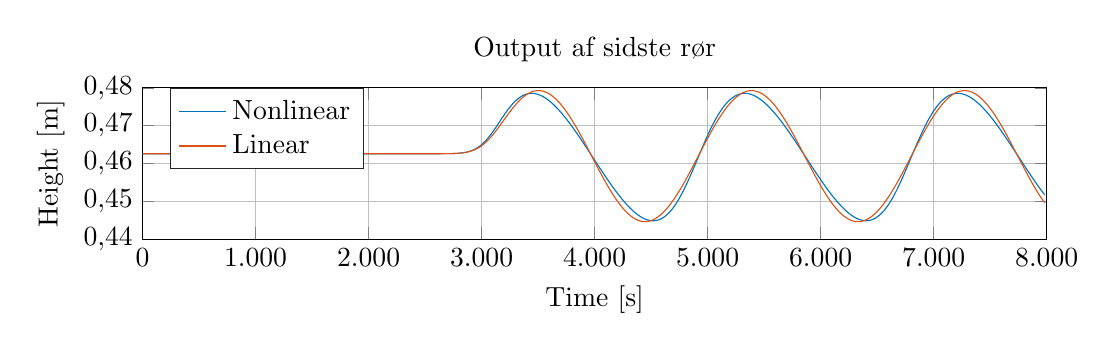
\begin{tikzpicture}

\begin{axis}[%
/pgf/number format/1000 sep={.},/pgf/number format/use comma,
width=4.521in,
height=.7566in,
at={(0.758in,0.481in)},
title ={Output af sidste rør},
scale only axis,
xmin=0,
xmax=8000,
xlabel={Time [s]},
xmajorgrids,
ymin=0.44,
ymax=0.48,
ylabel={Height [m]},
ymajorgrids,
axis background/.style={fill=white},
legend style={at={(0.03,0.73)},anchor=west},
legend style={legend cell align=left,align=left,draw=white!15!black}
]
\addplot [color=mycolor1,solid]
  table[row sep=crcr]{%
1	0.462595737606136\\
21	0.462595766861512\\
41	0.462595788438212\\
61	0.462595804181262\\
81	0.462595814989754\\
101	0.462595822807541\\
121	0.462595828630341\\
141	0.462595831905002\\
161	0.46259583412694\\
181	0.462595835844178\\
201	0.46259583699152\\
221	0.462595837729411\\
241	0.462595838185094\\
261	0.462595838461284\\
281	0.462595838623183\\
301	0.462595838711559\\
321	0.462595838750496\\
341	0.462595838752465\\
361	0.462595838721921\\
381	0.4625958386577\\
401	0.462595838554844\\
421	0.462595838406286\\
441	0.462595838204706\\
461	0.462595837944688\\
481	0.462595837625152\\
501	0.462595837251777\\
521	0.462595836838943\\
541	0.462595836410552\\
561	0.462595835999083\\
581	0.462595835642428\\
601	0.462595835378522\\
621	0.462595835238424\\
641	0.462595835239241\\
661	0.462595835378802\\
681	0.46259583563429\\
701	0.462595835965956\\
721	0.462595836326009\\
741	0.46259583667134\\
761	0.4625958369772\\
781	0.4625958372469\\
801	0.462595837510601\\
821	0.462595837811341\\
841	0.462595838185321\\
861	0.462595838646099\\
881	0.462595839178928\\
901	0.462595839745095\\
921	0.46259584029132\\
941	0.462595840759923\\
961	0.462595841098575\\
981	0.462595841269344\\
1001	0.462595841255849\\
1021	0.462595841066583\\
1041	0.462595840733295\\
1061	0.462595840304786\\
1081	0.462595839837555\\
1101	0.462595839385396\\
1121	0.462595838990585\\
1141	0.46259583867887\\
1161	0.462595838458964\\
1181	0.462595838325511\\
1201	0.462595838263768\\
1221	0.462595838254625\\
1241	0.46259583827901\\
1261	0.462595838320843\\
1281	0.462595838368157\\
1301	0.462595838412909\\
1321	0.462595838450395\\
1341	0.462595838478712\\
1361	0.462595838498255\\
1381	0.462595838511093\\
1401	0.462595838520255\\
1421	0.462595838528997\\
1441	0.46259583854018\\
1461	0.462595838555826\\
1481	0.462595838576902\\
1501	0.462595838603326\\
1521	0.462595838634151\\
1541	0.462595838667868\\
1561	0.462595838702734\\
1581	0.462595838737085\\
1601	0.462595838769557\\
1621	0.462595838799224\\
1641	0.462595838825622\\
1661	0.462595838848708\\
1681	0.462595838868759\\
1701	0.462595838886248\\
1721	0.462595838901721\\
1741	0.462595838915697\\
1761	0.462595838928591\\
1781	0.462595838940672\\
1801	0.462595838952052\\
1821	0.462595838962696\\
1841	0.462595838972448\\
1861	0.462595838981077\\
1881	0.462595838988318\\
1901	0.462595838993921\\
1921	0.462595838997697\\
1941	0.462595838999561\\
1961	0.462595838999575\\
1981	0.46259583899799\\
2001	0.462595838995287\\
2021	0.462595838992234\\
2041	0.462595838989955\\
2061	0.462595838990038\\
2081	0.462595838994679\\
2101	0.462595839006901\\
2121	0.462595839030852\\
2141	0.462595839072207\\
2161	0.46259583913876\\
2181	0.462595839241085\\
2201	0.462595839393452\\
2221	0.46259583961568\\
2241	0.462595839932888\\
2261	0.462595840379253\\
2281	0.462595841008547\\
2301	0.462595841858163\\
2321	0.462595843019391\\
2341	0.462595845638368\\
2361	0.4625958503106\\
2381	0.462595859125907\\
2401	0.462595874224808\\
2421	0.462595900568092\\
2441	0.46259594452641\\
2461	0.462596017209568\\
2481	0.462596133918965\\
2501	0.46259631785381\\
2521	0.462596599644938\\
2541	0.462597020085767\\
2561	0.462597629452957\\
2581	0.462598485211012\\
2601	0.462599653291652\\
2621	0.462601211614999\\
2641	0.462603270910744\\
2661	0.462606029337465\\
2681	0.462609870904031\\
2701	0.462615503569196\\
2721	0.462624112607928\\
2741	0.46263746573282\\
2761	0.462657927696744\\
2781	0.462688381305962\\
2801	0.462732126967519\\
2821	0.462792864345572\\
2841	0.462874800132007\\
2861	0.462982841012624\\
2881	0.463122751733321\\
2901	0.463301164887028\\
2921	0.463525383693851\\
2941	0.46380298787616\\
2961	0.464141275319514\\
2981	0.464546603824099\\
3001	0.465023723738187\\
3021	0.465575183944166\\
3041	0.466200875608223\\
3061	0.46689772826717\\
3081	0.467659571541626\\
3101	0.468477192712524\\
3121	0.469338619310273\\
3141	0.470229627253143\\
3161	0.471134437404302\\
3181	0.472036545221497\\
3201	0.472919622001497\\
3221	0.473768403009473\\
3241	0.474569438513391\\
3261	0.475311578027022\\
3281	0.475986128991952\\
3301	0.476586746354644\\
3321	0.477109177892581\\
3341	0.477550972074841\\
3361	0.477911178826543\\
3381	0.478190045081274\\
3401	0.478388723973582\\
3421	0.478509035502311\\
3441	0.478553294684254\\
3461	0.478524182145815\\
3481	0.478424623537686\\
3501	0.478257655473047\\
3521	0.478026314785805\\
3541	0.477733602173121\\
3561	0.47738254089049\\
3581	0.476976268333965\\
3601	0.476518060397594\\
3621	0.476011245130712\\
3641	0.47545904309026\\
3661	0.474864444741386\\
3681	0.474230207689763\\
3701	0.473558971311616\\
3721	0.472853408563272\\
3741	0.472116313052822\\
3761	0.471350571701492\\
3781	0.470559055223807\\
3801	0.469744502902326\\
3821	0.46890945975873\\
3841	0.468056279308506\\
3861	0.467187177240587\\
3881	0.466304314240948\\
3901	0.465409881535387\\
3921	0.464506158709552\\
3941	0.463595522263966\\
3961	0.462680405309402\\
3981	0.461763228435224\\
4001	0.460846328385924\\
4021	0.459931908983245\\
4041	0.459022034624202\\
4061	0.458118676734636\\
4081	0.457223800806582\\
4101	0.456339455804367\\
4121	0.455467824654186\\
4141	0.454611226317651\\
4161	0.453772100251186\\
4181	0.452953008380687\\
4201	0.452156648696482\\
4221	0.451385836185714\\
4241	0.450643426029038\\
4261	0.449932219537888\\
4281	0.449254929113725\\
4301	0.448614234014938\\
4321	0.448012878569118\\
4341	0.447453739908417\\
4361	0.446939839558729\\
4381	0.44647434512201\\
4401	0.446060595554607\\
4421	0.445702133914107\\
4441	0.445402706742644\\
4461	0.445166217376767\\
4481	0.444996657184716\\
4501	0.444898049706583\\
4521	0.444874383117409\\
4541	0.44492951658114\\
4561	0.445067050035481\\
4581	0.445290221202826\\
4601	0.445601871076422\\
4621	0.446004444523707\\
4641	0.446499957370417\\
4661	0.447089881838418\\
4681	0.447774969484852\\
4701	0.448555042272362\\
4721	0.449428783250223\\
4741	0.450393554823214\\
4761	0.45144526123565\\
4781	0.452578251837083\\
4801	0.453785262092848\\
4821	0.455057437346058\\
4841	0.456384522015529\\
4861	0.457755226755352\\
4881	0.459157658479834\\
4901	0.460579627094341\\
4921	0.462008752073201\\
4941	0.463432475906272\\
4961	0.464838171688495\\
4981	0.466213456263541\\
5001	0.467546667482304\\
5021	0.468827352513423\\
5041	0.470046586556222\\
5061	0.471197030174627\\
5081	0.472272770363773\\
5101	0.47326907833629\\
5121	0.474182212148699\\
5141	0.475009326281446\\
5161	0.475748486206027\\
5181	0.476398737917896\\
5201	0.476960143226998\\
5221	0.477433691431886\\
5241	0.477821069930187\\
5261	0.478124357961283\\
5281	0.478345765912584\\
5301	0.478487512168895\\
5321	0.478551852779087\\
5341	0.478541225105437\\
5361	0.478458394214516\\
5381	0.478306501319248\\
5401	0.478088959216268\\
5421	0.477809253818152\\
5441	0.477470786118439\\
5461	0.477076832102931\\
5481	0.47663058647073\\
5501	0.476135203510236\\
5521	0.475593780336078\\
5541	0.475009322157177\\
5561	0.474384750282148\\
5581	0.473722950736162\\
5601	0.473026799430022\\
5621	0.472299112843751\\
5641	0.471542551269154\\
5661	0.470759559127656\\
5681	0.469952405277727\\
5701	0.469123311086455\\
5721	0.46827459196725\\
5741	0.467408727973271\\
5761	0.466528318390822\\
5781	0.465635944291262\\
5801	0.464734028972795\\
5821	0.463824799057408\\
5841	0.462910378851767\\
5861	0.461992942586901\\
5881	0.46107480193166\\
5901	0.460158366463992\\
5921	0.459246018746161\\
5941	0.458339996203401\\
5961	0.457442349924919\\
5981	0.456555007564153\\
6001	0.455679931876339\\
6021	0.454819317892116\\
6041	0.453975716454362\\
6061	0.453151976708548\\
6081	0.452351008301765\\
6101	0.451575506849199\\
6121	0.45082783219231\\
6141	0.45011012604789\\
6161	0.44942459097568\\
6181	0.448773759457978\\
6201	0.448160613471587\\
6221	0.447588521960639\\
6241	0.447061063222956\\
6261	0.446581841206566\\
6281	0.446154386327256\\
6301	0.445782158282598\\
6321	0.445468610966842\\
6341	0.445217263297646\\
6361	0.445031741841928\\
6381	0.444915805522321\\
6401	0.444873351165655\\
6421	0.444908375095223\\
6441	0.445024827615758\\
6461	0.445226374670698\\
6481	0.44551615481219\\
6501	0.445896648950466\\
6521	0.446369693538927\\
6541	0.446936551429178\\
6561	0.447597931288157\\
6581	0.448353893073814\\
6601	0.449203647859668\\
6621	0.450145285496265\\
6641	0.451175466306077\\
6661	0.452289145414588\\
6681	0.453479432844087\\
6701	0.454737664462013\\
6721	0.456053668294621\\
6741	0.457416125332722\\
6761	0.458812927152067\\
6781	0.460231491336431\\
6801	0.46165905732883\\
6821	0.463082994401577\\
6841	0.464491098548183\\
6861	0.465871807792967\\
6881	0.467214296420706\\
6901	0.468508496672756\\
6921	0.469745148426169\\
6941	0.470915920459634\\
6961	0.472013588267787\\
6981	0.473032219475206\\
7001	0.473967322860057\\
7021	0.47481590339856\\
7041	0.475576347428661\\
7061	0.476248121577524\\
7081	0.476831397634691\\
7101	0.477326787330237\\
7121	0.477735296963816\\
7141	0.478058431459727\\
7161	0.478298287415192\\
7181	0.478457505420165\\
7201	0.478539068078455\\
7221	0.478546037683092\\
7241	0.478481356255522\\
7261	0.478347811075521\\
7281	0.47814814757116\\
7301	0.477885233336003\\
7321	0.477562154680077\\
7341	0.47718219234894\\
7361	0.476748713890495\\
7381	0.476265061745663\\
7401	0.475734478814768\\
7421	0.475160074919235\\
7441	0.474544828462544\\
7461	0.473891618610476\\
7481	0.473203272704271\\
7501	0.472482591551528\\
7521	0.47173231978675\\
7541	0.470955075285571\\
7561	0.470153299337239\\
7581	0.469329283635555\\
7601	0.468485269260669\\
7621	0.46762355399642\\
7641	0.46674654299248\\
7661	0.465856729240419\\
7681	0.464956638572598\\
7701	0.464048776136871\\
7721	0.46313558283631\\
7741	0.462219395731453\\
7761	0.461302419061183\\
7781	0.460386724760111\\
7801	0.459474291527016\\
7821	0.458567071551398\\
7841	0.457667064714051\\
7861	0.456776382674666\\
7881	0.4558972891119\\
7901	0.455032205739806\\
7921	0.454183683091857\\
7941	0.453354349456739\\
7961	0.452546859370056\\
7981	0.451763857819755\\
};
\addlegendentry{Nonlinear};

\addplot [color=mycolor2,solid]
  table[row sep=crcr]{%
1	0.462595737606136\\
21	0.462595737606136\\
41	0.462595737606136\\
61	0.462595737606136\\
81	0.462595737606136\\
101	0.462595737606136\\
121	0.462595737606136\\
141	0.462595737606136\\
161	0.462595737606136\\
181	0.462595737606136\\
201	0.462595737606136\\
221	0.462595737606136\\
241	0.462595737606136\\
261	0.462595737606136\\
281	0.462595737606136\\
301	0.462595737606136\\
321	0.462595737606136\\
341	0.462595737606136\\
361	0.462595737606136\\
381	0.462595737606136\\
401	0.462595737606136\\
421	0.462595737606136\\
441	0.462595737606136\\
461	0.462595737606136\\
481	0.462595737606136\\
501	0.462595737606136\\
521	0.462595737606136\\
541	0.462595737606136\\
561	0.462595737606136\\
581	0.462595737606136\\
601	0.462595737606136\\
621	0.462595737606136\\
641	0.462595737606136\\
661	0.462595737606136\\
681	0.462595737606136\\
701	0.462595737606136\\
721	0.462595737606136\\
741	0.462595737606136\\
761	0.462595737606136\\
781	0.462595737606136\\
801	0.462595737606136\\
821	0.462595737606136\\
841	0.462595737606136\\
861	0.462595737606136\\
881	0.462595737606136\\
901	0.462595737606136\\
921	0.462595737606136\\
941	0.462595737606136\\
961	0.462595737606136\\
981	0.462595737606136\\
1001	0.462595737606136\\
1021	0.462595737606136\\
1041	0.462595737606136\\
1061	0.462595737606136\\
1081	0.462595737606136\\
1101	0.462595737606136\\
1121	0.462595737606136\\
1141	0.462595737606136\\
1161	0.462595737606136\\
1181	0.462595737606136\\
1201	0.462595737606136\\
1221	0.462595737606136\\
1241	0.462595737606136\\
1261	0.462595737606136\\
1281	0.462595737606136\\
1301	0.462595737606136\\
1321	0.462595737606136\\
1341	0.462595737606136\\
1361	0.462595737606136\\
1381	0.462595737606136\\
1401	0.462595737606136\\
1421	0.462595737606136\\
1441	0.462595737606136\\
1461	0.462595737606136\\
1481	0.462595737606136\\
1501	0.462595737606136\\
1521	0.462595737606136\\
1541	0.462595737606136\\
1561	0.462595737606136\\
1581	0.462595737606136\\
1601	0.462595737606136\\
1621	0.462595737606136\\
1641	0.462595737606136\\
1661	0.462595737606136\\
1681	0.462595737606136\\
1701	0.462595737606136\\
1721	0.462595737606136\\
1741	0.462595737606136\\
1761	0.462595737606136\\
1781	0.462595737606136\\
1801	0.462595737606136\\
1821	0.462595737606136\\
1841	0.462595737606136\\
1861	0.462595737606136\\
1881	0.462595737606136\\
1901	0.462595737606136\\
1921	0.462595737606136\\
1941	0.462595737606136\\
1961	0.462595737606136\\
1981	0.462595737606136\\
2001	0.462595737606136\\
2021	0.462595737606136\\
2041	0.462595737606137\\
2061	0.462595737606138\\
2081	0.462595737606143\\
2101	0.462595737606155\\
2121	0.462595737606185\\
2141	0.46259573760626\\
2161	0.462595737606442\\
2181	0.462595737606881\\
2201	0.462595737607915\\
2221	0.462595737610311\\
2241	0.462595737615764\\
2261	0.462595737627956\\
2281	0.462595737654733\\
2301	0.462595737712507\\
2321	0.462595737834964\\
2341	0.462595738089961\\
2361	0.462595738611605\\
2381	0.462595739659966\\
2401	0.462595741729845\\
2421	0.462595745744776\\
2441	0.462595753395649\\
2461	0.462595767718986\\
2481	0.46259579406274\\
2501	0.462595841663183\\
2521	0.462595926160661\\
2541	0.46259607351919\\
2561	0.462596325986425\\
2581	0.462596750931272\\
2601	0.462597453611603\\
2621	0.462598595125208\\
2641	0.462600416936953\\
2661	0.462603273389091\\
2681	0.462607673407811\\
2701	0.462614332126884\\
2721	0.462624232274053\\
2741	0.462638693851075\\
2761	0.462659448883477\\
2781	0.462688715905299\\
2801	0.462729266569813\\
2821	0.462784474648894\\
2841	0.462858336113408\\
2861	0.462955448443918\\
2881	0.463080938255977\\
2901	0.463240329068703\\
2921	0.463439345704039\\
2941	0.463683658163351\\
2961	0.463978575310206\\
2981	0.464328706373438\\
3001	0.46473761501669\\
3021	0.465207495286579\\
3041	0.465738900112641\\
3061	0.466330550555491\\
3081	0.466979247640297\\
3101	0.467679898990943\\
3121	0.468425660825992\\
3141	0.469208183838434\\
3161	0.470017940829825\\
3181	0.470844606270707\\
3201	0.471677454272659\\
3221	0.472505742144354\\
3241	0.473319051383251\\
3261	0.474107565612145\\
3281	0.474862274193669\\
3301	0.475575099532513\\
3321	0.476238954078418\\
3341	0.476847738850598\\
3361	0.47739629850329\\
3381	0.477880348625895\\
3401	0.478296389589548\\
3421	0.47864161850588\\
3441	0.478913847491583\\
3461	0.479111433077405\\
3481	0.479233218721608\\
3501	0.479278490232898\\
3521	0.479246942531599\\
3541	0.479138655495855\\
3561	0.478954076489315\\
3581	0.478694007363406\\
3601	0.478359594104554\\
3621	0.47795231772777\\
3641	0.477473985421703\\
3661	0.476926721285119\\
3681	0.476312956249171\\
3701	0.475635416959559\\
3721	0.474897113512448\\
3741	0.474101326013728\\
3761	0.473251589977429\\
3781	0.472351680606591\\
3801	0.47140559601645\\
3821	0.470417539470096\\
3841	0.46939190070374\\
3861	0.468333236423857\\
3881	0.467246250062632\\
3901	0.46613577088155\\
3921	0.46500673251596\\
3941	0.463864151055931\\
3961	0.462713102760771\\
3981	0.461558701506231\\
4001	0.460406076064587\\
4021	0.459260347318534\\
4041	0.45812660551014\\
4061	0.45700988762592\\
4081	0.455915155018524\\
4101	0.454847271364446\\
4121	0.453810981055686\\
4141	0.452810888121376\\
4161	0.451851435773001\\
4181	0.450936886664109\\
4201	0.450071303952199\\
4221	0.44925853324693\\
4241	0.448502185524851\\
4261	0.447805621086561\\
4281	0.44717193462757\\
4301	0.446603941489189\\
4321	0.446104165150538\\
4341	0.445674826017232\\
4361	0.445317831556572\\
4381	0.445034767823046\\
4401	0.444826892411812\\
4421	0.444695128871457\\
4441	0.444640062600852\\
4461	0.444661938248348\\
4481	0.444760658624848\\
4501	0.444935785135602\\
4521	0.445186539728794\\
4541	0.445511808352268\\
4561	0.445910145903041\\
4581	0.446379782647601\\
4601	0.446918632084476\\
4621	0.447524300214145\\
4641	0.448194096175091\\
4661	0.448925044198757\\
4681	0.449713896830289\\
4701	0.450557149356322\\
4721	0.451451055375714\\
4741	0.452391643444058\\
4761	0.453374734718002\\
4781	0.454395961521012\\
4801	0.45545078674808\\
4821	0.456534524023167\\
4841	0.457642358519826\\
4861	0.458769368352508\\
4881	0.459910546443511\\
4901	0.461060822768411\\
4921	0.462215086881164\\
4941	0.46336821061879\\
4961	0.464515070884764\\
4981	0.465650572409904\\
5001	0.466769670389626\\
5021	0.467867392896996\\
5041	0.468938862971997\\
5061	0.469979320288883\\
5081	0.470984142305344\\
5101	0.471948864799536\\
5121	0.472869201703713\\
5141	0.473741064146368\\
5161	0.474560578618265\\
5181	0.475324104181655\\
5201	0.476028248646237\\
5221	0.476669883639971\\
5241	0.477246158507807\\
5261	0.477754512976569\\
5281	0.478192688529737\\
5301	0.478558738441577\\
5321	0.478851036426055\\
5341	0.479068283862095\\
5361	0.479209515563092\\
5381	0.479274104065045\\
5401	0.479261762414245\\
5421	0.479172545442164\\
5441	0.479006849521838\\
5461	0.478765410806871\\
5481	0.478449301960847\\
5501	0.478059927391703\\
5521	0.47759901701223\\
5541	0.477068618554415\\
5561	0.476471088471782\\
5581	0.475809081470146\\
5601	0.475085538713283\\
5621	0.474303674755941\\
5641	0.473466963262213\\
5661	0.472579121572749\\
5681	0.471644094189362\\
5701	0.470666035250401\\
5721	0.469649290074747\\
5741	0.468598375856442\\
5761	0.4675179615957\\
5781	0.466412847355485\\
5801	0.465287942935794\\
5821	0.464148246060404\\
5841	0.462998820172995\\
5861	0.461844771941289\\
5881	0.460691228569151\\
5901	0.459543315017457\\
5921	0.458406131234925\\
5941	0.457284729500069\\
5961	0.456184091974945\\
5981	0.455109108570406\\
6001	0.454064555221213\\
6021	0.453055072667523\\
6041	0.452085145837008\\
6061	0.451159083919233\\
6081	0.450281001220785\\
6101	0.449454798886248\\
6121	0.448684147566193\\
6141	0.447972471109226\\
6161	0.447322931350511\\
6181	0.446738414064377\\
6201	0.446221516143404\\
6221	0.44577453406095\\
6241	0.445399453668385\\
6261	0.44509794137235\\
6281	0.444871336731251\\
6301	0.44472064650387\\
6321	0.444646540176539\\
6341	0.444649346988744\\
6361	0.444729054470383\\
6381	0.44488530849717\\
6401	0.445117414863933\\
6421	0.445424342368832\\
6441	0.445804727394777\\
6461	0.446256879967709\\
6481	0.446778791264812\\
6501	0.447368142539305\\
6521	0.448022315422174\\
6541	0.448738403555052\\
6561	0.449513225502585\\
6581	0.450343338886913\\
6601	0.451225055681454\\
6621	0.452154458596072\\
6641	0.453127418480799\\
6661	0.454139612670824\\
6681	0.45518654419122\\
6701	0.456263561736095\\
6721	0.457365880333411\\
6741	0.45848860260365\\
6761	0.459626740517885\\
6781	0.460775237558584\\
6801	0.461928991184708\\
6821	0.463082875501263\\
6841	0.464231764032626\\
6861	0.46537055249844\\
6881	0.466494181490907\\
6901	0.467597658952714\\
6921	0.468676082355742\\
6941	0.469724660482008\\
6961	0.470738734710082\\
6981	0.471713799712407\\
7001	0.472645523471557\\
7021	0.473529766526521\\
7041	0.474362600363495\\
7061	0.475140324869477\\
7081	0.47585948477112\\
7101	0.476516884985823\\
7121	0.477109604816833\\
7141	0.477635010929317\\
7161	0.478090769049734\\
7181	0.478474854336547\\
7201	0.478785560376182\\
7221	0.479021506764281\\
7241	0.479181645238563\\
7261	0.479265264336037\\
7281	0.479271992553897\\
7301	0.479201800000023\\
7321	0.479054998525797\\
7341	0.478832240340602\\
7361	0.478534515114191\\
7381	0.478163145579783\\
7401	0.477719781657424\\
7421	0.477206393123726\\
7441	0.476625260860548\\
7461	0.475978966721493\\
7481	0.475270382061256\\
7501	0.474502654978772\\
7521	0.473679196330847\\
7541	0.472803664578406\\
7561	0.471879949532692\\
7581	0.470912155073615\\
7601	0.46990458091704\\
7621	0.468861703512017\\
7641	0.467788156152819\\
7661	0.466688708394148\\
7681	0.465568244860965\\
7701	0.464431743547083\\
7721	0.463284253698947\\
7741	0.462130873382844\\
7761	0.460976726835226\\
7781	0.459826941696755\\
7801	0.458686626231234\\
7821	0.457560846630612\\
7841	0.456454604506922\\
7861	0.455372814671118\\
7881	0.454320283297567\\
7901	0.453301686571179\\
7921	0.452321549912062\\
7941	0.451384227869991\\
7961	0.450493884778019\\
7981	0.449654476251187\\
};
\addlegendentry{Linear};

\end{axis}
\end{tikzpicture}%
%\caption{Comparison of the nonlinear and linear model at the last pipe in the setup.}
\label{fig:linear_nonlinear_comparison_last_pipe}
\end{figure}
\vspace{5mm}
\vfill \vfill
\end{frame}

\subsection{MPC}

\begin{frame}{Kontrol}{MPC}
    \vfill\vfill\centering
\begin{itemize}
	\item Cost funktion
	\begin{itemize}
		\item Afgrænset til at minimiere flow variationer
	\end{itemize}
	\item Constraints
	\begin{itemize}
		\item Højde
		\item Kontrol input
	\end{itemize}
	\item Prediktions model
\end{itemize}
\vfill\vfill
\end{frame}





\begin{frame}{Kontrol}{MPC}
  \vfill\vfill\centering



      \begin{minipage}[t]{0.48\linewidth}
    \begin{itemize}
    %	\item Bestemmelse af Prediction horizon
    	% \begin{itemize}
    	% 	\item Flow profiler
    	% 	\item Industri 
    	% \end{itemize}
    	\item Begrænset i længde af prediktions horisont
    	\item System setup
    	\item Forstyrrelses input
    \end{itemize}  
    \vspace{4mm}
    	 \begin{figure}
	 \centering
	 % This file was created by matlab2tikz.
%
%The latest updates can be retrieved from
%  http://www.mathworks.com/matlabcentral/fileexchange/22022-matlab2tikz-matlab2tikz
%where you can also make suggestions and rate matlab2tikz.
%
\definecolor{mycolor1}{rgb}{0.00000,0.44700,0.74100}%
%
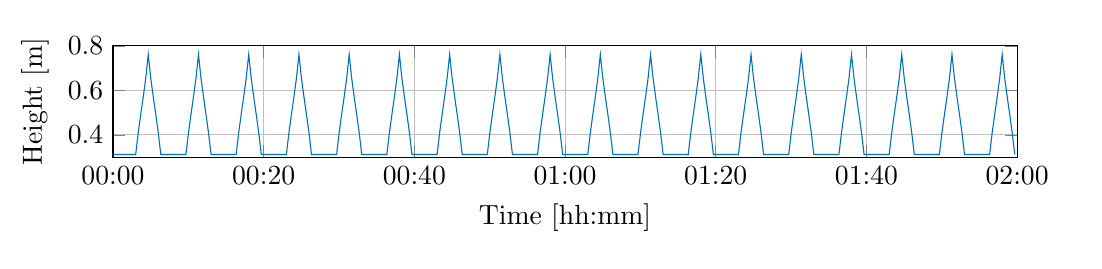
\begin{tikzpicture}
\vspace{5mm}
\hspace{-2mm}
\begin{axis}[%
width=4.521in,
height=.5566in,
at={(0.758in,0.481in)},
scale only axis,
xmin=0,
xmax=7200,
xtick={0,1200,2400,3600,4800,6000,7200},
xticklabels={{00:00},{00:20},{00:40},{01:00},{01:20},{01:40},{02:00},{},{}},
xlabel={Time [hh:mm]},
xmajorgrids,
ymin=0.3,
ymax=0.8,
ylabel={Height [m]},
ymajorgrids,
axis background/.style={fill=white}
]
\addplot [color=mycolor1,solid,forget plot]
  table[row sep=crcr]{%
1	0.31203\\
21	0.31203\\
41	0.31203\\
61	0.31203\\
81	0.31203\\
101	0.31203\\
121	0.31203\\
141	0.31203\\
161	0.31203\\
181	0.31203\\
201	0.40851\\
221	0.49122\\
241	0.57033\\
261	0.65412\\
281	0.76113\\
301	0.65412\\
321	0.57033\\
341	0.49122\\
361	0.40851\\
381	0.31203\\
401	0.31203\\
421	0.31203\\
441	0.31203\\
461	0.31203\\
481	0.31203\\
501	0.31203\\
521	0.31203\\
541	0.31203\\
561	0.31203\\
581	0.31203\\
601	0.40851\\
621	0.49122\\
641	0.57033\\
661	0.65412\\
681	0.76113\\
701	0.65412\\
721	0.57033\\
741	0.49122\\
761	0.40851\\
781	0.31203\\
801	0.31203\\
821	0.31203\\
841	0.31203\\
861	0.31203\\
881	0.31203\\
901	0.31203\\
921	0.31203\\
941	0.31203\\
961	0.31203\\
981	0.31203\\
1001	0.40851\\
1021	0.49122\\
1041	0.57033\\
1061	0.65412\\
1081	0.76113\\
1101	0.65412\\
1121	0.57033\\
1141	0.49122\\
1161	0.40851\\
1181	0.31203\\
1201	0.31203\\
1221	0.31203\\
1241	0.31203\\
1261	0.31203\\
1281	0.31203\\
1301	0.31203\\
1321	0.31203\\
1341	0.31203\\
1361	0.31203\\
1381	0.31203\\
1401	0.40851\\
1421	0.49122\\
1441	0.57033\\
1461	0.65412\\
1481	0.76113\\
1501	0.65412\\
1521	0.57033\\
1541	0.49122\\
1561	0.40851\\
1581	0.31203\\
1601	0.31203\\
1621	0.31203\\
1641	0.31203\\
1661	0.31203\\
1681	0.31203\\
1701	0.31203\\
1721	0.31203\\
1741	0.31203\\
1761	0.31203\\
1781	0.31203\\
1801	0.40851\\
1821	0.49122\\
1841	0.57033\\
1861	0.65412\\
1881	0.76113\\
1901	0.65412\\
1921	0.57033\\
1941	0.49122\\
1961	0.40851\\
1981	0.31203\\
2001	0.31203\\
2021	0.31203\\
2041	0.31203\\
2061	0.31203\\
2081	0.31203\\
2101	0.31203\\
2121	0.31203\\
2141	0.31203\\
2161	0.31203\\
2181	0.31203\\
2201	0.40851\\
2221	0.49122\\
2241	0.57033\\
2261	0.65412\\
2281	0.76113\\
2301	0.65412\\
2321	0.57033\\
2341	0.49122\\
2361	0.40851\\
2381	0.31203\\
2401	0.31203\\
2421	0.31203\\
2441	0.31203\\
2461	0.31203\\
2481	0.31203\\
2501	0.31203\\
2521	0.31203\\
2541	0.31203\\
2561	0.31203\\
2581	0.31203\\
2601	0.40851\\
2621	0.49122\\
2641	0.57033\\
2661	0.65412\\
2681	0.76113\\
2701	0.65412\\
2721	0.57033\\
2741	0.49122\\
2761	0.40851\\
2781	0.31203\\
2801	0.31203\\
2821	0.31203\\
2841	0.31203\\
2861	0.31203\\
2881	0.31203\\
2901	0.31203\\
2921	0.31203\\
2941	0.31203\\
2961	0.31203\\
2981	0.31203\\
3001	0.40851\\
3021	0.49122\\
3041	0.57033\\
3061	0.65412\\
3081	0.76113\\
3101	0.65412\\
3121	0.57033\\
3141	0.49122\\
3161	0.40851\\
3181	0.31203\\
3201	0.31203\\
3221	0.31203\\
3241	0.31203\\
3261	0.31203\\
3281	0.31203\\
3301	0.31203\\
3321	0.31203\\
3341	0.31203\\
3361	0.31203\\
3381	0.31203\\
3401	0.40851\\
3421	0.49122\\
3441	0.57033\\
3461	0.65412\\
3481	0.76113\\
3501	0.65412\\
3521	0.57033\\
3541	0.49122\\
3561	0.40851\\
3581	0.31203\\
3601	0.31203\\
3621	0.31203\\
3641	0.31203\\
3661	0.31203\\
3681	0.31203\\
3701	0.31203\\
3721	0.31203\\
3741	0.31203\\
3761	0.31203\\
3781	0.31203\\
3801	0.40851\\
3821	0.49122\\
3841	0.57033\\
3861	0.65412\\
3881	0.76113\\
3901	0.65412\\
3921	0.57033\\
3941	0.49122\\
3961	0.40851\\
3981	0.31203\\
4001	0.31203\\
4021	0.31203\\
4041	0.31203\\
4061	0.31203\\
4081	0.31203\\
4101	0.31203\\
4121	0.31203\\
4141	0.31203\\
4161	0.31203\\
4181	0.31203\\
4201	0.40851\\
4221	0.49122\\
4241	0.57033\\
4261	0.65412\\
4281	0.76113\\
4301	0.65412\\
4321	0.57033\\
4341	0.49122\\
4361	0.40851\\
4381	0.31203\\
4401	0.31203\\
4421	0.31203\\
4441	0.31203\\
4461	0.31203\\
4481	0.31203\\
4501	0.31203\\
4521	0.31203\\
4541	0.31203\\
4561	0.31203\\
4581	0.31203\\
4601	0.40851\\
4621	0.49122\\
4641	0.57033\\
4661	0.65412\\
4681	0.76113\\
4701	0.65412\\
4721	0.57033\\
4741	0.49122\\
4761	0.40851\\
4781	0.31203\\
4801	0.31203\\
4821	0.31203\\
4841	0.31203\\
4861	0.31203\\
4881	0.31203\\
4901	0.31203\\
4921	0.31203\\
4941	0.31203\\
4961	0.31203\\
4981	0.31203\\
5001	0.40851\\
5021	0.49122\\
5041	0.57033\\
5061	0.65412\\
5081	0.76113\\
5101	0.65412\\
5121	0.57033\\
5141	0.49122\\
5161	0.40851\\
5181	0.31203\\
5201	0.31203\\
5221	0.31203\\
5241	0.31203\\
5261	0.31203\\
5281	0.31203\\
5301	0.31203\\
5321	0.31203\\
5341	0.31203\\
5361	0.31203\\
5381	0.31203\\
5401	0.40851\\
5421	0.49122\\
5441	0.57033\\
5461	0.65412\\
5481	0.76113\\
5501	0.65412\\
5521	0.57033\\
5541	0.49122\\
5561	0.40851\\
5581	0.31203\\
5601	0.31203\\
5621	0.31203\\
5641	0.31203\\
5661	0.31203\\
5681	0.31203\\
5701	0.31203\\
5721	0.31203\\
5741	0.31203\\
5761	0.31203\\
5781	0.31203\\
5801	0.40851\\
5821	0.49122\\
5841	0.57033\\
5861	0.65412\\
5881	0.76113\\
5901	0.65412\\
5921	0.57033\\
5941	0.49122\\
5961	0.40851\\
5981	0.31203\\
6001	0.31203\\
6021	0.31203\\
6041	0.31203\\
6061	0.31203\\
6081	0.31203\\
6101	0.31203\\
6121	0.31203\\
6141	0.31203\\
6161	0.31203\\
6181	0.31203\\
6201	0.40851\\
6221	0.49122\\
6241	0.57033\\
6261	0.65412\\
6281	0.76113\\
6301	0.65412\\
6321	0.57033\\
6341	0.49122\\
6361	0.40851\\
6381	0.31203\\
6401	0.31203\\
6421	0.31203\\
6441	0.31203\\
6461	0.31203\\
6481	0.31203\\
6501	0.31203\\
6521	0.31203\\
6541	0.31203\\
6561	0.31203\\
6581	0.31203\\
6601	0.40851\\
6621	0.49122\\
6641	0.57033\\
6661	0.65412\\
6681	0.76113\\
6701	0.65412\\
6721	0.57033\\
6741	0.49122\\
6761	0.40851\\
6781	0.31203\\
6801	0.31203\\
6821	0.31203\\
6841	0.31203\\
6861	0.31203\\
6881	0.31203\\
6901	0.31203\\
6921	0.31203\\
6941	0.31203\\
6961	0.31203\\
6981	0.31203\\
7001	0.40851\\
7021	0.49122\\
7041	0.57033\\
7061	0.65412\\
7081	0.76113\\
7101	0.65412\\
7121	0.57033\\
7141	0.49122\\
7161	0.40851\\
7181	0.31203\\
};
\end{axis}
\end{tikzpicture}%
	%\caption{Output of the last pipe.}
	\label{fig:MPC_test_o}
	\end{figure}  
\end{minipage}\hfill
\begin{minipage}[t]{0.48\linewidth}
\begin{figure}[!h]
\centering
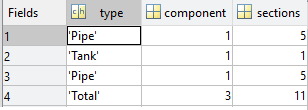
\includegraphics[width=0.97 \textwidth]{figures/mpc_system_setup}
%\caption{Setup in MATLAB of pipe specification of the main line in Fredericia.}
\label{fig:mpc_system_setup}
\end{figure}

\end{minipage}


\vfill\vfill
\end{frame}

\begin{frame}{Kontrol}{MPC}
	\vfill\vfill \centering
	\vspace{-6mm}
	 \begin{figure}
	 \centering
	 % This file was created by matlab2tikz.
%
%The latest updates can be retrieved from
%  http://www.mathworks.com/matlabcentral/fileexchange/22022-matlab2tikz-matlab2tikz
%where you can also make suggestions and rate matlab2tikz.
%
\definecolor{mycolor1}{rgb}{0.00000,0.44700,0.74100}%
%
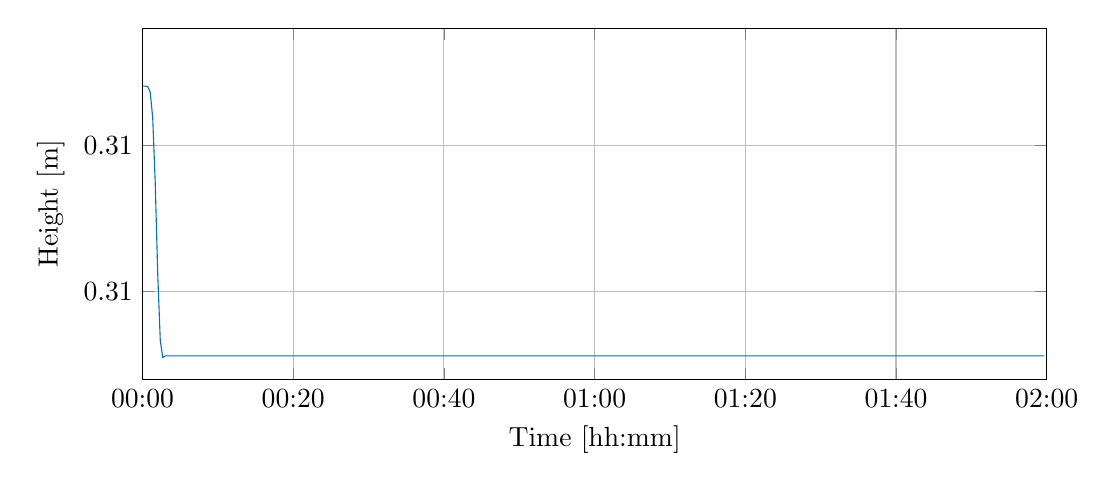
\begin{tikzpicture}

\begin{axis}[%
width=4.521in,
height=1.7566in,
at={(0.758in,0.481in)},
scale only axis,
xmin=0,
xmax=7200,
xtick={0,1200,2400,3600,4800,6000,7200},
xticklabels={{00:00},{00:20},{00:40},{01:00},{01:20},{01:40},{02:00},{},{}},
xlabel={Time [hh:mm]},
xmajorgrids,
ymin=0.302,
ymax=0.314,
ylabel={Height [m]},
ymajorgrids,
axis background/.style={fill=white}
]
\addplot [color=mycolor1,solid,forget plot]
  table[row sep=crcr]{%
1	0.312023251728134\\
21	0.312023249248491\\
41	0.312007329576048\\
61	0.311822355594219\\
81	0.310938012057319\\
101	0.308710026090253\\
121	0.305594844450276\\
141	0.303344739104071\\
161	0.302753859420006\\
181	0.302809429127008\\
201	0.30280716177161\\
221	0.302807232518793\\
241	0.302807230514799\\
261	0.302807230566105\\
281	0.30280723056466\\
301	0.302807230564718\\
321	0.302807230564717\\
341	0.302807230564717\\
361	0.302807230564717\\
381	0.302807230564717\\
401	0.302807230564717\\
421	0.302807230564717\\
441	0.302807230564717\\
461	0.302807230564717\\
481	0.302807230564717\\
501	0.302807230564717\\
521	0.302807230564717\\
541	0.302807230564717\\
561	0.302807230564717\\
581	0.302807230564717\\
601	0.302807230564717\\
621	0.302807230564717\\
641	0.302807230564717\\
661	0.302807230564717\\
681	0.302807230564717\\
701	0.302807230564717\\
721	0.302807230564717\\
741	0.302807230564717\\
761	0.302807230564717\\
781	0.302807230564717\\
801	0.302807230564717\\
821	0.302807230564717\\
841	0.302807230564717\\
861	0.302807230564717\\
881	0.302807230564717\\
901	0.302807230564717\\
921	0.302807230564717\\
941	0.302807230564717\\
961	0.302807230564717\\
981	0.302807230564717\\
1001	0.302807230564717\\
1021	0.302807230564717\\
1041	0.302807230564717\\
1061	0.302807230564717\\
1081	0.302807230564717\\
1101	0.302807230564717\\
1121	0.302807230564717\\
1141	0.302807230564717\\
1161	0.302807230564717\\
1181	0.302807230564717\\
1201	0.302807230564717\\
1221	0.302807230564717\\
1241	0.302807230564717\\
1261	0.302807230564717\\
1281	0.302807230564717\\
1301	0.302807230564717\\
1321	0.302807230564717\\
1341	0.302807230564717\\
1361	0.302807230564717\\
1381	0.302807230564717\\
1401	0.302807230564717\\
1421	0.302807230564717\\
1441	0.302807230564717\\
1461	0.302807230564717\\
1481	0.302807230564717\\
1501	0.302807230564717\\
1521	0.302807230564717\\
1541	0.302807230564717\\
1561	0.302807230564717\\
1581	0.302807230564717\\
1601	0.302807230564717\\
1621	0.302807230564717\\
1641	0.302807230564717\\
1661	0.302807230564717\\
1681	0.302807230564717\\
1701	0.302807230564717\\
1721	0.302807230564717\\
1741	0.302807230564717\\
1761	0.302807230564717\\
1781	0.302807230564717\\
1801	0.302807230564717\\
1821	0.302807230564717\\
1841	0.302807230564717\\
1861	0.302807230564717\\
1881	0.302807230564717\\
1901	0.302807230564717\\
1921	0.302807230564717\\
1941	0.302807230564717\\
1961	0.302807230564717\\
1981	0.302807230564717\\
2001	0.302807230564717\\
2021	0.302807230564717\\
2041	0.302807230564717\\
2061	0.302807230564717\\
2081	0.302807230564717\\
2101	0.302807230564717\\
2121	0.302807230564717\\
2141	0.302807230564717\\
2161	0.302807230564717\\
2181	0.302807230564717\\
2201	0.302807230564717\\
2221	0.302807230564717\\
2241	0.302807230564717\\
2261	0.302807230564717\\
2281	0.302807230564717\\
2301	0.302807230564717\\
2321	0.302807230564717\\
2341	0.302807230564717\\
2361	0.302807230564717\\
2381	0.302807230564717\\
2401	0.302807230564717\\
2421	0.302807230564717\\
2441	0.302807230564717\\
2461	0.302807230564717\\
2481	0.302807230564717\\
2501	0.302807230564717\\
2521	0.302807230564717\\
2541	0.302807230564717\\
2561	0.302807230564717\\
2581	0.302807230564717\\
2601	0.302807230564717\\
2621	0.302807230564717\\
2641	0.302807230564717\\
2661	0.302807230564717\\
2681	0.302807230564717\\
2701	0.302807230564717\\
2721	0.302807230564717\\
2741	0.302807230564717\\
2761	0.302807230564717\\
2781	0.302807230564717\\
2801	0.302807230564717\\
2821	0.302807230564717\\
2841	0.302807230564717\\
2861	0.302807230564717\\
2881	0.302807230564717\\
2901	0.302807230564717\\
2921	0.302807230564717\\
2941	0.302807230564717\\
2961	0.302807230564717\\
2981	0.302807230564717\\
3001	0.302807230564717\\
3021	0.302807230564717\\
3041	0.302807230564717\\
3061	0.302807230564717\\
3081	0.302807230564717\\
3101	0.302807230564717\\
3121	0.302807230564717\\
3141	0.302807230564717\\
3161	0.302807230564717\\
3181	0.302807230564717\\
3201	0.302807230564717\\
3221	0.302807230564717\\
3241	0.302807230564717\\
3261	0.302807230564717\\
3281	0.302807230564717\\
3301	0.302807230564717\\
3321	0.302807230564717\\
3341	0.302807230564717\\
3361	0.302807230564717\\
3381	0.302807230564717\\
3401	0.302807230564717\\
3421	0.302807230564717\\
3441	0.302807230564717\\
3461	0.302807230564717\\
3481	0.302807230564717\\
3501	0.302807230564717\\
3521	0.302807230564717\\
3541	0.302807230564717\\
3561	0.302807230564717\\
3581	0.302807230564717\\
3601	0.302807230564717\\
3621	0.302807230564717\\
3641	0.302807230564717\\
3661	0.302807230564717\\
3681	0.302807230564717\\
3701	0.302807230564717\\
3721	0.302807230564717\\
3741	0.302807230564717\\
3761	0.302807230564717\\
3781	0.302807230564717\\
3801	0.302807230564717\\
3821	0.302807230564717\\
3841	0.302807230564717\\
3861	0.302807230564717\\
3881	0.302807230564717\\
3901	0.302807230564717\\
3921	0.302807230564717\\
3941	0.302807230564717\\
3961	0.302807230564717\\
3981	0.302807230564717\\
4001	0.302807230564717\\
4021	0.302807230564717\\
4041	0.302807230564717\\
4061	0.302807230564717\\
4081	0.302807230564717\\
4101	0.302807230564717\\
4121	0.302807230564717\\
4141	0.302807230564717\\
4161	0.302807230564717\\
4181	0.302807230564717\\
4201	0.302807230564717\\
4221	0.302807230564717\\
4241	0.302807230564717\\
4261	0.302807230564717\\
4281	0.302807230564717\\
4301	0.302807230564717\\
4321	0.302807230564717\\
4341	0.302807230564717\\
4361	0.302807230564717\\
4381	0.302807230564717\\
4401	0.302807230564717\\
4421	0.302807230564717\\
4441	0.302807230564717\\
4461	0.302807230564717\\
4481	0.302807230564717\\
4501	0.302807230564717\\
4521	0.302807230564717\\
4541	0.302807230564717\\
4561	0.302807230564717\\
4581	0.302807230564717\\
4601	0.302807230564717\\
4621	0.302807230564717\\
4641	0.302807230564717\\
4661	0.302807230564717\\
4681	0.302807230564717\\
4701	0.302807230564717\\
4721	0.302807230564717\\
4741	0.302807230564717\\
4761	0.302807230564717\\
4781	0.302807230564717\\
4801	0.302807230564717\\
4821	0.302807230564717\\
4841	0.302807230564717\\
4861	0.302807230564717\\
4881	0.302807230564717\\
4901	0.302807230564717\\
4921	0.302807230564717\\
4941	0.302807230564717\\
4961	0.302807230564717\\
4981	0.302807230564717\\
5001	0.302807230564717\\
5021	0.302807230564717\\
5041	0.302807230564717\\
5061	0.302807230564717\\
5081	0.302807230564717\\
5101	0.302807230564717\\
5121	0.302807230564717\\
5141	0.302807230564717\\
5161	0.302807230564717\\
5181	0.302807230564717\\
5201	0.302807230564717\\
5221	0.302807230564717\\
5241	0.302807230564717\\
5261	0.302807230564717\\
5281	0.302807230564717\\
5301	0.302807230564717\\
5321	0.302807230564717\\
5341	0.302807230564717\\
5361	0.302807230564717\\
5381	0.302807230564717\\
5401	0.302807230564717\\
5421	0.302807230564717\\
5441	0.302807230564717\\
5461	0.302807230564717\\
5481	0.302807230564717\\
5501	0.302807230564717\\
5521	0.302807230564717\\
5541	0.302807230564717\\
5561	0.302807230564717\\
5581	0.302807230564717\\
5601	0.302807230564717\\
5621	0.302807230564717\\
5641	0.302807230564717\\
5661	0.302807230564717\\
5681	0.302807230564717\\
5701	0.302807230564717\\
5721	0.302807230564717\\
5741	0.302807230564717\\
5761	0.302807230564717\\
5781	0.302807230564717\\
5801	0.302807230564717\\
5821	0.302807230564717\\
5841	0.302807230564717\\
5861	0.302807230564717\\
5881	0.302807230564717\\
5901	0.302807230564717\\
5921	0.302807230564717\\
5941	0.302807230564717\\
5961	0.302807230564717\\
5981	0.302807230564717\\
6001	0.302807230564717\\
6021	0.302807230564717\\
6041	0.302807230564717\\
6061	0.302807230564717\\
6081	0.302807230564717\\
6101	0.302807230564717\\
6121	0.302807230564717\\
6141	0.302807230564717\\
6161	0.302807230564717\\
6181	0.302807230564717\\
6201	0.302807230564717\\
6221	0.302807230564717\\
6241	0.302807230564717\\
6261	0.302807230564717\\
6281	0.302807230564717\\
6301	0.302807230564717\\
6321	0.302807230564717\\
6341	0.302807230564717\\
6361	0.302807230564717\\
6381	0.302807230564717\\
6401	0.302807230564717\\
6421	0.302807230564717\\
6441	0.302807230564717\\
6461	0.302807230564717\\
6481	0.302807230564717\\
6501	0.302807230564717\\
6521	0.302807230564717\\
6541	0.302807230564717\\
6561	0.302807230564717\\
6581	0.302807230564717\\
6601	0.302807230564717\\
6621	0.302807230564717\\
6641	0.302807230564717\\
6661	0.302807230564717\\
6681	0.302807230564717\\
6701	0.302807230564717\\
6721	0.302807230564717\\
6741	0.302807230564717\\
6761	0.302807230564717\\
6781	0.302807230564717\\
6801	0.302807230564717\\
6821	0.302807230564717\\
6841	0.302807230564717\\
6861	0.302807230564717\\
6881	0.302807230564717\\
6901	0.302807230564717\\
6921	0.302807230564717\\
6941	0.302807230564717\\
6961	0.302807230564717\\
6981	0.302807230564717\\
7001	0.302807230564717\\
7021	0.302807230564717\\
7041	0.302807230564717\\
7061	0.302807230564717\\
7081	0.302807230564717\\
7101	0.302807230564717\\
7121	0.302807230564717\\
7141	0.302807230564717\\
7161	0.302807230564717\\
7181	0.302807230564717\\
};
\end{axis}
\end{tikzpicture}%
	%\caption{Output of the last pipe.}
	\label{fig:MPC_test_output_first_test}
	\end{figure}   
	\vspace{-10mm}
	\begin{figure}
	 \centering
	 % This file was created by matlab2tikz.
%
%The latest updates can be retrieved from
%  http://www.mathworks.com/matlabcentral/fileexchange/22022-matlab2tikz-matlab2tikz
%where you can also make suggestions and rate matlab2tikz.
%
\definecolor{mycolor1}{rgb}{0.00000,0.44700,0.74100}%
%
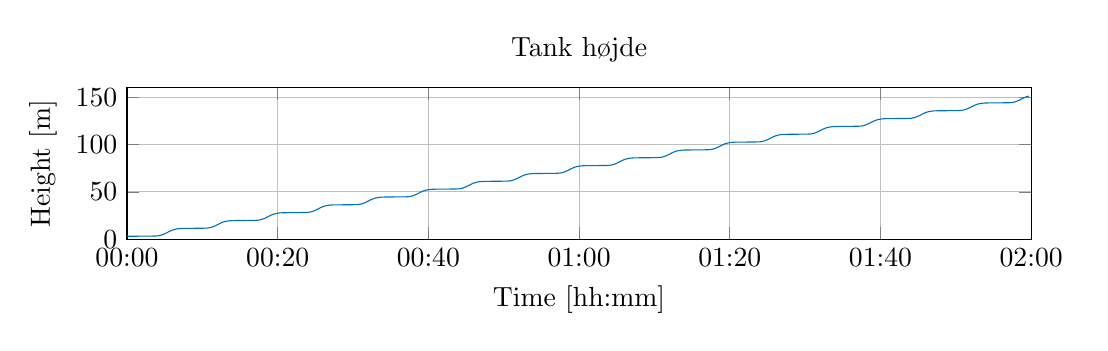
\begin{tikzpicture}
\hspace{-1mm}
\begin{axis}[%
width=4.521in,
height=.7566in,
at={(0.758in,0.481in)},
scale only axis,
xmin=0,
xmax=7200,
title ={Tank højde},
xtick={0,1200,2400,3600,4800,6000,7200},
xticklabels={{00:00},{00:20},{00:40},{01:00},{01:20},{01:40},{02:00},{},{}},
xlabel={Time [hh:mm]},
xmajorgrids,
ymin=-0.1,
ymax=160,
ylabel={Height [m]},
ymajorgrids,
axis background/.style={fill=white}
]
\addplot [color=mycolor1,solid,forget plot]
  table[row sep=crcr]{%
1	3\\
21	2.99999999316026\\
41	3.01333332012207\\
61	3.03959998125893\\
81	3.06547864251583\\
101	3.0913689429355\\
121	3.11725889387259\\
141	3.14314885534856\\
161	3.16903881650788\\
181	3.19492877767658\\
201	3.22208190892336\\
221	3.26581919849303\\
241	3.40261431116685\\
261	3.80277617108737\\
281	4.582895898918\\
301	5.68730591534825\\
321	7.00239347163539\\
341	8.36007404320854\\
361	9.51275135815108\\
381	10.3267153588503\\
401	10.8543133136161\\
421	11.1590600902295\\
441	11.2945893110534\\
461	11.3388672109703\\
481	11.3608410656606\\
501	11.3869549591855\\
521	11.4128355845539\\
541	11.4387258658624\\
561	11.4646158173399\\
581	11.4905057788189\\
601	11.5176589100695\\
621	11.5613961996392\\
641	11.698191312313\\
661	12.0983531722335\\
681	12.8784729000642\\
701	13.9828829164944\\
721	15.2979704727815\\
741	16.6556510443547\\
761	17.8083283592972\\
781	18.6222923599965\\
801	19.1498903147623\\
821	19.4546370913756\\
841	19.5901663121995\\
861	19.6344442121164\\
881	19.6564180668067\\
901	19.6825319603317\\
921	19.7084125857001\\
941	19.7343028670085\\
961	19.7601928184861\\
981	19.7860827799651\\
1001	19.8132359112157\\
1021	19.8569732007853\\
1041	19.9937683134592\\
1061	20.3939301733797\\
1081	21.1740499012103\\
1101	22.2784599176406\\
1121	23.5935474739277\\
1141	24.9512280455008\\
1161	26.1039053604434\\
1181	26.9178693611426\\
1201	27.4454673159084\\
1221	27.7502140925218\\
1241	27.8857433133457\\
1261	27.9300212132626\\
1281	27.9519950679529\\
1301	27.9781089614778\\
1321	28.0039895868462\\
1341	28.0298798681547\\
1361	28.0557698196322\\
1381	28.0816597811112\\
1401	28.1088129123618\\
1421	28.1525502019315\\
1441	28.2893453146053\\
1461	28.6895071745258\\
1481	29.4696269023564\\
1501	30.5740369187867\\
1521	31.8891244750738\\
1541	33.246805046647\\
1561	34.3994823615895\\
1581	35.2134463622888\\
1601	35.7410443170546\\
1621	36.0457910936679\\
1641	36.1813203144918\\
1661	36.2255982144087\\
1681	36.247572069099\\
1701	36.273685962624\\
1721	36.2995665879924\\
1741	36.3254568693008\\
1761	36.3513468207784\\
1781	36.3772367822573\\
1801	36.404389913508\\
1821	36.4481272030776\\
1841	36.5849223157514\\
1861	36.985084175672\\
1881	37.7652039035026\\
1901	38.8696139199329\\
1921	40.18470147622\\
1941	41.5423820477931\\
1961	42.6950593627357\\
1981	43.5090233634349\\
2001	44.0366213182008\\
2021	44.3413680948141\\
2041	44.476897315638\\
2061	44.5211752155549\\
2081	44.5431490702452\\
2101	44.5692629637701\\
2121	44.5951435891385\\
2141	44.621033870447\\
2161	44.6469238219245\\
2181	44.6728137834035\\
2201	44.6999669146541\\
2221	44.7437042042238\\
2241	44.8804993168976\\
2261	45.2806611768181\\
2281	46.0607809046488\\
2301	47.165190921079\\
2321	48.4802784773661\\
2341	49.8379590489393\\
2361	50.9906363638818\\
2381	51.8046003645811\\
2401	52.3321983193469\\
2421	52.6369450959602\\
2441	52.7724743167841\\
2461	52.816752216701\\
2481	52.8387260713913\\
2501	52.8648399649163\\
2521	52.8907205902847\\
2541	52.9166108715932\\
2561	52.9425008230707\\
2581	52.9683907845497\\
2601	52.9955439158003\\
2621	53.0392812053699\\
2641	53.1760763180438\\
2661	53.5762381779643\\
2681	54.3563579057949\\
2701	55.4607679222252\\
2721	56.7758554785123\\
2741	58.1335360500855\\
2761	59.286213365028\\
2781	60.1001773657272\\
2801	60.6277753204931\\
2821	60.9325220971064\\
2841	61.0680513179303\\
2861	61.1123292178472\\
2881	61.1343030725375\\
2901	61.1604169660624\\
2921	61.1862975914308\\
2941	61.2121878727393\\
2961	61.2380778242168\\
2981	61.2639677856958\\
3001	61.2911209169465\\
3021	61.3348582065161\\
3041	61.4716533191899\\
3061	61.8718151791104\\
3081	62.6519349069411\\
3101	63.7563449233713\\
3121	65.0714324796585\\
3141	66.4291130512316\\
3161	67.5817903661741\\
3181	68.3957543668734\\
3201	68.9233523216392\\
3221	69.2280990982525\\
3241	69.3636283190764\\
3261	69.4079062189933\\
3281	69.4298800736836\\
3301	69.4559939672086\\
3321	69.481874592577\\
3341	69.5077648738854\\
3361	69.533654825363\\
3381	69.559544786842\\
3401	69.5866979180926\\
3421	69.6304352076622\\
3441	69.7672303203361\\
3461	70.1673921802566\\
3481	70.9475119080872\\
3501	72.0519219245175\\
3521	73.3670094808046\\
3541	74.7246900523778\\
3561	75.8773673673203\\
3581	76.6913313680195\\
3601	77.2189293227854\\
3621	77.5236760993987\\
3641	77.6592053202226\\
3661	77.7034832201395\\
3681	77.7254570748298\\
3701	77.7515709683547\\
3721	77.7774515937231\\
3741	77.8033418750316\\
3761	77.8292318265091\\
3781	77.8551217879881\\
3801	77.8822749192387\\
3821	77.9260122088084\\
3841	78.0628073214822\\
3861	78.4629691814027\\
3881	79.2430889092334\\
3901	80.3474989256636\\
3921	81.6625864819507\\
3941	83.0202670535239\\
3961	84.1729443684664\\
3981	84.9869083691657\\
4001	85.5145063239315\\
4021	85.8192531005448\\
4041	85.9547823213687\\
4061	85.9990602212856\\
4081	86.0210340759759\\
4101	86.0471479695009\\
4121	86.0730285948693\\
4141	86.0989188761777\\
4161	86.1248088276553\\
4181	86.1506987891342\\
4201	86.1778519203849\\
4221	86.2215892099545\\
4241	86.3583843226283\\
4261	86.7585461825489\\
4281	87.5386659103795\\
4301	88.6430759268097\\
4321	89.9581634830969\\
4341	91.31584405467\\
4361	92.4685213696126\\
4381	93.2824853703118\\
4401	93.8100833250776\\
4421	94.114830101691\\
4441	94.2503593225149\\
4461	94.2946372224318\\
4481	94.3166110771221\\
4501	94.342724970647\\
4521	94.3686055960154\\
4541	94.3944958773239\\
4561	94.4203858288014\\
4581	94.4462757902804\\
4601	94.473428921531\\
4621	94.5171662111007\\
4641	94.6539613237745\\
4661	95.054123183695\\
4681	95.8342429115256\\
4701	96.9386529279559\\
4721	98.253740484243\\
4741	99.6114210558162\\
4761	100.764098370759\\
4781	101.578062371458\\
4801	102.105660326224\\
4821	102.410407102837\\
4841	102.545936323661\\
4861	102.590214223578\\
4881	102.612188078268\\
4901	102.638301971793\\
4921	102.664182597162\\
4941	102.69007287847\\
4961	102.715962829948\\
4981	102.741852791427\\
5001	102.769005922677\\
5021	102.812743212247\\
5041	102.949538324921\\
5061	103.349700184841\\
5081	104.129819912672\\
5101	105.234229929102\\
5121	106.549317485389\\
5141	107.906998056962\\
5161	109.059675371905\\
5181	109.873639372604\\
5201	110.40123732737\\
5221	110.705984103983\\
5241	110.841513324807\\
5261	110.885791224724\\
5281	110.907765079414\\
5301	110.933878972939\\
5321	110.959759598308\\
5341	110.985649879616\\
5361	111.011539831094\\
5381	111.037429792573\\
5401	111.064582923823\\
5421	111.108320213393\\
5441	111.245115326067\\
5461	111.645277185987\\
5481	112.425396913818\\
5501	113.529806930248\\
5521	114.844894486535\\
5541	116.202575058108\\
5561	117.355252373051\\
5581	118.16921637375\\
5601	118.696814328516\\
5621	119.001561105129\\
5641	119.137090325953\\
5661	119.18136822587\\
5681	119.203342080561\\
5701	119.229455974085\\
5721	119.255336599454\\
5741	119.281226880762\\
5761	119.30711683224\\
5781	119.333006793719\\
5801	119.360159924969\\
5821	119.403897214539\\
5841	119.540692327213\\
5861	119.940854187133\\
5881	120.720973914964\\
5901	121.825383931394\\
5921	123.140471487681\\
5941	124.498152059255\\
5961	125.650829374197\\
5981	126.464793374896\\
6001	126.992391329662\\
6021	127.297138106276\\
6041	127.432667327099\\
6061	127.476945227016\\
6081	127.498919081707\\
6101	127.525032975232\\
6121	127.5509136006\\
6141	127.576803881908\\
6161	127.602693833386\\
6181	127.628583794865\\
6201	127.655736926116\\
6221	127.699474215685\\
6241	127.836269328359\\
6261	128.23643118828\\
6281	129.01655091611\\
6301	130.12096093254\\
6321	131.436048488828\\
6341	132.793729060401\\
6361	133.946406375343\\
6381	134.760370376042\\
6401	135.287968330808\\
6421	135.592715107422\\
6441	135.728244328246\\
6461	135.772522228162\\
6481	135.794496082853\\
6501	135.820609976378\\
6521	135.846490601746\\
6541	135.872380883055\\
6561	135.898270834532\\
6581	135.924160796011\\
6601	135.951313927262\\
6621	135.995051216831\\
6641	136.131846329505\\
6661	136.532008189426\\
6681	137.312127917256\\
6701	138.416537933687\\
6721	139.731625489974\\
6741	141.089306061547\\
6761	142.241983376489\\
6781	143.055947377189\\
6801	143.583545331955\\
6821	143.888292108568\\
6841	144.023821329392\\
6861	144.068099229309\\
6881	144.090073083999\\
6901	144.116186977524\\
6921	144.142067602892\\
6941	144.167957884201\\
6961	144.193847835678\\
6981	144.219737797157\\
7001	144.246890928408\\
7021	144.290628217978\\
7041	144.427423330651\\
7061	144.827585190572\\
7081	145.607704918403\\
7101	146.712114934833\\
7121	148.02720249112\\
7141	149.384883062693\\
7161	150.537560377636\\
7181	151.351524378335\\
};
\end{axis}
\end{tikzpicture}%
	%\caption{Height in the tank.}
	\label{fig:tank_height_first_test}
	\end{figure} 
	\vfill\vfill
\end{frame}


\begin{frame}{Kontrol}{MPC}
\vspace{-6mm}
	 \begin{figure}
	 \centering
	 % This file was created by matlab2tikz.
%
%The latest updates can be retrieved from
%  http://www.mathworks.com/matlabcentral/fileexchange/22022-matlab2tikz-matlab2tikz
%where you can also make suggestions and rate matlab2tikz.
%
\definecolor{mycolor1}{rgb}{0.00000,0.44700,0.74100}%
%
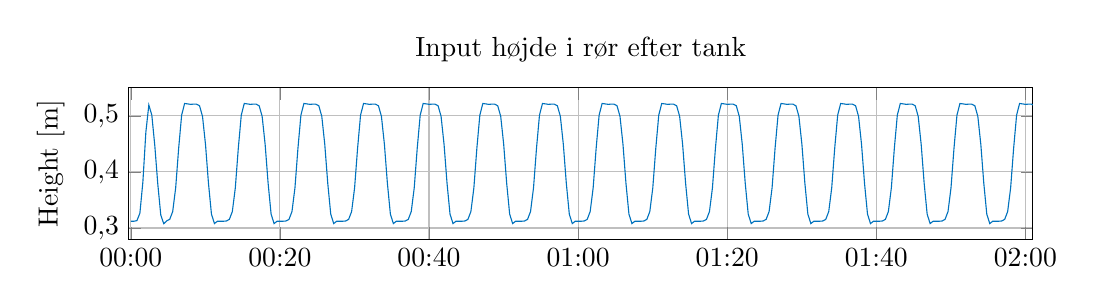
\begin{tikzpicture}

\begin{axis}[%
/pgf/number format/1000 sep={.},/pgf/number format/use comma,
width=4.521in,
height=.7566in,
at={(0.758in,0.481in)},
scale only axis,
xmin=-13.9733315078526,
title={Input højde i rør efter tank },
xmax=6050.45254290018,
xtick={0,1000,2000,3000,4000,5000,6000,7000,8000},
xticklabels={{00:00},{00:20},{00:40},{01:00},{01:20},{01:40},{02:00},{},{}},
%xlabel={Time [hh:mm]},
xmajorgrids,
ymin=0.28,
ymax=0.55,
ylabel={Height [m]},
ymajorgrids,
axis background/.style={fill=white}
]
\addplot [color=mycolor1,solid,forget plot]
  table[row sep=crcr]{%
1	0.312023251728134\\
21	0.312023249248491\\
41	0.313138414051669\\
61	0.326407936305141\\
81	0.381997703162978\\
101	0.470815867610163\\
121	0.519510061802365\\
141	0.501318732196232\\
161	0.446991990334918\\
181	0.378629775152903\\
201	0.323425157927926\\
221	0.307611772797364\\
241	0.312704231743349\\
261	0.315364784289658\\
281	0.329313448452517\\
301	0.371599902771225\\
321	0.442036405727331\\
341	0.501390997061537\\
361	0.522134625957773\\
381	0.521439921581776\\
401	0.520589133516734\\
421	0.520996119305126\\
441	0.520882715260118\\
461	0.518086829318264\\
481	0.499148503119224\\
501	0.449201077704583\\
521	0.379770972259138\\
541	0.324785916393953\\
561	0.307879632744135\\
581	0.312048759866851\\
601	0.31204380765778\\
621	0.31205923660724\\
641	0.312471245607916\\
661	0.315374578361834\\
681	0.329313094015343\\
701	0.371599917605447\\
721	0.44203640471571\\
741	0.501390997170403\\
761	0.522134625943674\\
781	0.52143992158365\\
801	0.520589133516488\\
821	0.520996119305158\\
841	0.520882715260114\\
861	0.518086829318264\\
881	0.499148503119224\\
901	0.449201077704583\\
921	0.379770972259138\\
941	0.324785916393953\\
961	0.307879632744135\\
981	0.312048759866851\\
1001	0.31204380765778\\
1021	0.31205923660724\\
1041	0.312471245607916\\
1061	0.315374578361834\\
1081	0.329313094015343\\
1101	0.371599917605447\\
1121	0.44203640471571\\
1141	0.501390997170403\\
1161	0.522134625943674\\
1181	0.52143992158365\\
1201	0.520589133516488\\
1221	0.520996119305158\\
1241	0.520882715260114\\
1261	0.518086829318264\\
1281	0.499148503119224\\
1301	0.449201077704583\\
1321	0.379770972259138\\
1341	0.324785916393953\\
1361	0.307879632744135\\
1381	0.312048759866851\\
1401	0.31204380765778\\
1421	0.31205923660724\\
1441	0.312471245607916\\
1461	0.315374578361834\\
1481	0.329313094015343\\
1501	0.371599917605447\\
1521	0.44203640471571\\
1541	0.501390997170403\\
1561	0.522134625943674\\
1581	0.52143992158365\\
1601	0.520589133516488\\
1621	0.520996119305158\\
1641	0.520882715260114\\
1661	0.518086829318264\\
1681	0.499148503119224\\
1701	0.449201077704583\\
1721	0.379770972259138\\
1741	0.324785916393953\\
1761	0.307879632744135\\
1781	0.312048759866851\\
1801	0.31204380765778\\
1821	0.31205923660724\\
1841	0.312471245607916\\
1861	0.315374578361834\\
1881	0.329313094015343\\
1901	0.371599917605447\\
1921	0.44203640471571\\
1941	0.501390997170403\\
1961	0.522134625943674\\
1981	0.52143992158365\\
2001	0.520589133516488\\
2021	0.520996119305158\\
2041	0.520882715260114\\
2061	0.518086829318264\\
2081	0.499148503119224\\
2101	0.449201077704583\\
2121	0.379770972259138\\
2141	0.324785916393953\\
2161	0.307879632744135\\
2181	0.312048759866851\\
2201	0.31204380765778\\
2221	0.31205923660724\\
2241	0.312471245607916\\
2261	0.315374578361834\\
2281	0.329313094015343\\
2301	0.371599917605447\\
2321	0.44203640471571\\
2341	0.501390997170403\\
2361	0.522134625943674\\
2381	0.52143992158365\\
2401	0.520589133516488\\
2421	0.520996119305158\\
2441	0.520882715260114\\
2461	0.518086829318264\\
2481	0.499148503119224\\
2501	0.449201077704583\\
2521	0.379770972259138\\
2541	0.324785916393953\\
2561	0.307879632744135\\
2581	0.312048759866851\\
2601	0.31204380765778\\
2621	0.31205923660724\\
2641	0.312471245607916\\
2661	0.315374578361834\\
2681	0.329313094015343\\
2701	0.371599917605447\\
2721	0.44203640471571\\
2741	0.501390997170403\\
2761	0.522134625943674\\
2781	0.52143992158365\\
2801	0.520589133516488\\
2821	0.520996119305158\\
2841	0.520882715260114\\
2861	0.518086829318264\\
2881	0.499148503119224\\
2901	0.449201077704583\\
2921	0.379770972259138\\
2941	0.324785916393953\\
2961	0.307879632744135\\
2981	0.312048759866851\\
3001	0.31204380765778\\
3021	0.31205923660724\\
3041	0.312471245607916\\
3061	0.315374578361834\\
3081	0.329313094015343\\
3101	0.371599917605447\\
3121	0.44203640471571\\
3141	0.501390997170403\\
3161	0.522134625943674\\
3181	0.52143992158365\\
3201	0.520589133516488\\
3221	0.520996119305158\\
3241	0.520882715260114\\
3261	0.518086829318264\\
3281	0.499148503119224\\
3301	0.449201077704583\\
3321	0.379770972259138\\
3341	0.324785916393953\\
3361	0.307879632744135\\
3381	0.312048759866851\\
3401	0.31204380765778\\
3421	0.31205923660724\\
3441	0.312471245607916\\
3461	0.315374578361834\\
3481	0.329313094015343\\
3501	0.371599917605447\\
3521	0.44203640471571\\
3541	0.501390997170403\\
3561	0.522134625943674\\
3581	0.52143992158365\\
3601	0.520589133516488\\
3621	0.520996119305158\\
3641	0.520882715260114\\
3661	0.518086829318264\\
3681	0.499148503119224\\
3701	0.449201077704583\\
3721	0.379770972259138\\
3741	0.324785916393953\\
3761	0.307879632744135\\
3781	0.312048759866851\\
3801	0.31204380765778\\
3821	0.31205923660724\\
3841	0.312471245607916\\
3861	0.315374578361834\\
3881	0.329313094015343\\
3901	0.371599917605447\\
3921	0.44203640471571\\
3941	0.501390997170403\\
3961	0.522134625943674\\
3981	0.52143992158365\\
4001	0.520589133516488\\
4021	0.520996119305158\\
4041	0.520882715260114\\
4061	0.518086829318264\\
4081	0.499148503119224\\
4101	0.449201077704583\\
4121	0.379770972259138\\
4141	0.324785916393953\\
4161	0.307879632744135\\
4181	0.312048759866851\\
4201	0.31204380765778\\
4221	0.31205923660724\\
4241	0.312471245607916\\
4261	0.315374578361834\\
4281	0.329313094015343\\
4301	0.371599917605447\\
4321	0.44203640471571\\
4341	0.501390997170403\\
4361	0.522134625943674\\
4381	0.52143992158365\\
4401	0.520589133516488\\
4421	0.520996119305158\\
4441	0.520882715260114\\
4461	0.518086829318264\\
4481	0.499148503119224\\
4501	0.449201077704583\\
4521	0.379770972259138\\
4541	0.324785916393953\\
4561	0.307879632744135\\
4581	0.312048759866851\\
4601	0.31204380765778\\
4621	0.31205923660724\\
4641	0.312471245607916\\
4661	0.315374578361834\\
4681	0.329313094015343\\
4701	0.371599917605447\\
4721	0.44203640471571\\
4741	0.501390997170403\\
4761	0.522134625943674\\
4781	0.52143992158365\\
4801	0.520589133516488\\
4821	0.520996119305158\\
4841	0.520882715260114\\
4861	0.518086829318264\\
4881	0.499148503119224\\
4901	0.449201077704583\\
4921	0.379770972259138\\
4941	0.324785916393953\\
4961	0.307879632744135\\
4981	0.312048759866851\\
5001	0.31204380765778\\
5021	0.31205923660724\\
5041	0.312471245607916\\
5061	0.315374578361834\\
5081	0.329313094015343\\
5101	0.371599917605447\\
5121	0.44203640471571\\
5141	0.501390997170403\\
5161	0.522134625943674\\
5181	0.52143992158365\\
5201	0.520589133516488\\
5221	0.520996119305158\\
5241	0.520882715260114\\
5261	0.518086829318264\\
5281	0.499148503119224\\
5301	0.449201077704583\\
5321	0.379770972259138\\
5341	0.324785916393953\\
5361	0.307879632744135\\
5381	0.312048759866851\\
5401	0.31204380765778\\
5421	0.31205923660724\\
5441	0.312471245607916\\
5461	0.315374578361834\\
5481	0.329313094015343\\
5501	0.371599917605447\\
5521	0.44203640471571\\
5541	0.501390997170403\\
5561	0.522134625943674\\
5581	0.52143992158365\\
5601	0.520589133516488\\
5621	0.520996119305158\\
5641	0.520882715260114\\
5661	0.518086829318264\\
5681	0.499148503119224\\
5701	0.449201077704583\\
5721	0.379770972259138\\
5741	0.324785916393953\\
5761	0.307879632744135\\
5781	0.312048759866851\\
5801	0.31204380765778\\
5821	0.31205923660724\\
5841	0.312471245607916\\
5861	0.315374578361834\\
5881	0.329313094015343\\
5901	0.371599917605447\\
5921	0.44203640471571\\
5941	0.501390997170403\\
5961	0.522134625943674\\
5981	0.52143992158365\\
6001	0.520589133516488\\
6021	0.520996119305158\\
6041	0.520882715260114\\
6061	0.518086829318264\\
};
\end{axis}
\end{tikzpicture}%
	%\caption{Output of the last pipe in the second Simulering run.}
	\label{fig:MPC_test_output_second_test_with_constraints}
	\end{figure}   
\vspace{-8mm}
	 \begin{figure}
	 \centering
	 % This file was created by matlab2tikz.
%
%The latest updates can be retrieved from
%  http://www.mathworks.com/matlabcentral/fileexchange/22022-matlab2tikz-matlab2tikz
%where you can also make suggestions and rate matlab2tikz.
%
\definecolor{mycolor1}{rgb}{0.00000,0.44700,0.74100}%
%
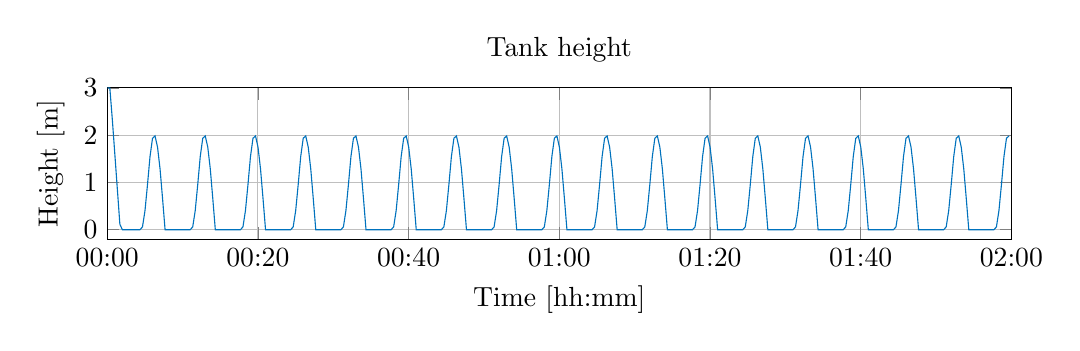
\begin{tikzpicture}

\begin{axis}[%
width=4.521in,
height=.7566in,
/pgf/number format/1000 sep={.},/pgf/number format/use comma,
at={(0.758in,0.481in)},
scale only axis,
xmin=0,
title={Tank height},
xmax=7200,
xtick={0,1200,2400,3600,4800,6000,7200},
xticklabels={{00:00},{00:20},{00:40},{01:00},{01:20},{01:40},{02:00},{},{}},
xlabel={Time [hh:mm]},
xmajorgrids,
ymin=-0.2,
ymax=3,
ylabel={Height [m]},
ymajorgrids,
axis background/.style={fill=white}
]
\addplot [color=mycolor1,solid,forget plot]
  table[row sep=crcr]{%
1	3\\
21	2.99999999316026\\
41	2.32754415169987\\
61	1.59384668206183\\
81	0.855486505639804\\
101	0.11665418915018\\
121	0\\
141	0\\
161	0\\
181	0\\
201	0\\
221	0\\
241	0\\
261	0\\
281	0.0595953504678914\\
301	0.40302542412948\\
321	0.953696376221655\\
341	1.54661857226603\\
361	1.93450659540532\\
381	1.98368241475169\\
401	1.74649216864076\\
421	1.28645074216793\\
441	0.6571917603094\\
461	0\\
481	0\\
501	0\\
521	0\\
541	0\\
561	0\\
581	0\\
601	0\\
621	0\\
641	0\\
661	0\\
681	0.0595953504680377\\
701	0.403025424129614\\
721	0.953696376221789\\
741	1.54661857226616\\
761	1.93450659540545\\
781	1.98368241475182\\
801	1.74649216864089\\
821	1.28645074216806\\
841	0.657191760309528\\
861	0\\
881	0\\
901	0\\
921	0\\
941	0\\
961	0\\
981	0\\
1001	0\\
1021	0\\
1041	0\\
1061	0\\
1081	0.0595953504680377\\
1101	0.403025424129614\\
1121	0.953696376221789\\
1141	1.54661857226616\\
1161	1.93450659540545\\
1181	1.98368241475182\\
1201	1.74649216864089\\
1221	1.28645074216806\\
1241	0.657191760309528\\
1261	0\\
1281	0\\
1301	0\\
1321	0\\
1341	0\\
1361	0\\
1381	0\\
1401	0\\
1421	0\\
1441	0\\
1461	0\\
1481	0.0595953504680377\\
1501	0.403025424129614\\
1521	0.953696376221789\\
1541	1.54661857226616\\
1561	1.93450659540545\\
1581	1.98368241475182\\
1601	1.74649216864089\\
1621	1.28645074216806\\
1641	0.657191760309528\\
1661	0\\
1681	0\\
1701	0\\
1721	0\\
1741	0\\
1761	0\\
1781	0\\
1801	0\\
1821	0\\
1841	0\\
1861	0\\
1881	0.0595953504680377\\
1901	0.403025424129614\\
1921	0.953696376221789\\
1941	1.54661857226616\\
1961	1.93450659540545\\
1981	1.98368241475182\\
2001	1.74649216864089\\
2021	1.28645074216806\\
2041	0.657191760309528\\
2061	0\\
2081	0\\
2101	0\\
2121	0\\
2141	0\\
2161	0\\
2181	0\\
2201	0\\
2221	0\\
2241	0\\
2261	0\\
2281	0.0595953504680377\\
2301	0.403025424129614\\
2321	0.953696376221789\\
2341	1.54661857226616\\
2361	1.93450659540545\\
2381	1.98368241475182\\
2401	1.74649216864089\\
2421	1.28645074216806\\
2441	0.657191760309528\\
2461	0\\
2481	0\\
2501	0\\
2521	0\\
2541	0\\
2561	0\\
2581	0\\
2601	0\\
2621	0\\
2641	0\\
2661	0\\
2681	0.0595953504680377\\
2701	0.403025424129614\\
2721	0.953696376221789\\
2741	1.54661857226616\\
2761	1.93450659540545\\
2781	1.98368241475182\\
2801	1.74649216864089\\
2821	1.28645074216806\\
2841	0.657191760309528\\
2861	0\\
2881	0\\
2901	0\\
2921	0\\
2941	0\\
2961	0\\
2981	0\\
3001	0\\
3021	0\\
3041	0\\
3061	0\\
3081	0.0595953504680377\\
3101	0.403025424129614\\
3121	0.953696376221789\\
3141	1.54661857226616\\
3161	1.93450659540545\\
3181	1.98368241475182\\
3201	1.74649216864089\\
3221	1.28645074216806\\
3241	0.657191760309528\\
3261	0\\
3281	0\\
3301	0\\
3321	0\\
3341	0\\
3361	0\\
3381	0\\
3401	0\\
3421	0\\
3441	0\\
3461	0\\
3481	0.0595953504680377\\
3501	0.403025424129614\\
3521	0.953696376221789\\
3541	1.54661857226616\\
3561	1.93450659540545\\
3581	1.98368241475182\\
3601	1.74649216864089\\
3621	1.28645074216806\\
3641	0.657191760309528\\
3661	0\\
3681	0\\
3701	0\\
3721	0\\
3741	0\\
3761	0\\
3781	0\\
3801	0\\
3821	0\\
3841	0\\
3861	0\\
3881	0.0595953504680377\\
3901	0.403025424129614\\
3921	0.953696376221789\\
3941	1.54661857226616\\
3961	1.93450659540545\\
3981	1.98368241475182\\
4001	1.74649216864089\\
4021	1.28645074216806\\
4041	0.657191760309528\\
4061	0\\
4081	0\\
4101	0\\
4121	0\\
4141	0\\
4161	0\\
4181	0\\
4201	0\\
4221	0\\
4241	0\\
4261	0\\
4281	0.0595953504680377\\
4301	0.403025424129614\\
4321	0.953696376221789\\
4341	1.54661857226616\\
4361	1.93450659540545\\
4381	1.98368241475182\\
4401	1.74649216864089\\
4421	1.28645074216806\\
4441	0.657191760309528\\
4461	0\\
4481	0\\
4501	0\\
4521	0\\
4541	0\\
4561	0\\
4581	0\\
4601	0\\
4621	0\\
4641	0\\
4661	0\\
4681	0.0595953504680377\\
4701	0.403025424129614\\
4721	0.953696376221789\\
4741	1.54661857226616\\
4761	1.93450659540545\\
4781	1.98368241475182\\
4801	1.74649216864089\\
4821	1.28645074216806\\
4841	0.657191760309528\\
4861	0\\
4881	0\\
4901	0\\
4921	0\\
4941	0\\
4961	0\\
4981	0\\
5001	0\\
5021	0\\
5041	0\\
5061	0\\
5081	0.0595953504680377\\
5101	0.403025424129614\\
5121	0.953696376221789\\
5141	1.54661857226616\\
5161	1.93450659540545\\
5181	1.98368241475182\\
5201	1.74649216864089\\
5221	1.28645074216806\\
5241	0.657191760309528\\
5261	0\\
5281	0\\
5301	0\\
5321	0\\
5341	0\\
5361	0\\
5381	0\\
5401	0\\
5421	0\\
5441	0\\
5461	0\\
5481	0.0595953504680377\\
5501	0.403025424129614\\
5521	0.953696376221789\\
5541	1.54661857226616\\
5561	1.93450659540545\\
5581	1.98368241475182\\
5601	1.74649216864089\\
5621	1.28645074216806\\
5641	0.657191760309528\\
5661	0\\
5681	0\\
5701	0\\
5721	0\\
5741	0\\
5761	0\\
5781	0\\
5801	0\\
5821	0\\
5841	0\\
5861	0\\
5881	0.0595953504680377\\
5901	0.403025424129614\\
5921	0.953696376221789\\
5941	1.54661857226616\\
5961	1.93450659540545\\
5981	1.98368241475182\\
6001	1.74649216864089\\
6021	1.28645074216806\\
6041	0.657191760309528\\
6061	0\\
6081	0\\
6101	0\\
6121	0\\
6141	0\\
6161	0\\
6181	0\\
6201	0\\
6221	0\\
6241	0\\
6261	0\\
6281	0.0595953504680377\\
6301	0.403025424129614\\
6321	0.953696376221789\\
6341	1.54661857226616\\
6361	1.93450659540545\\
6381	1.98368241475182\\
6401	1.74649216864089\\
6421	1.28645074216806\\
6441	0.657191760309528\\
6461	0\\
6481	0\\
6501	0\\
6521	0\\
6541	0\\
6561	0\\
6581	0\\
6601	0\\
6621	0\\
6641	0\\
6661	0\\
6681	0.0595953504680377\\
6701	0.403025424129614\\
6721	0.953696376221789\\
6741	1.54661857226616\\
6761	1.93450659540545\\
6781	1.98368241475182\\
6801	1.74649216864089\\
6821	1.28645074216806\\
6841	0.657191760309528\\
6861	0\\
6881	0\\
6901	0\\
6921	0\\
6941	0\\
6961	0\\
6981	0\\
7001	0\\
7021	0\\
7041	0\\
7061	0\\
7081	0.0595953504680377\\
7101	0.403025424129614\\
7121	0.953696376221789\\
7141	1.54661857226616\\
7161	1.93450659540545\\
7181	1.98368241475182\\
};
\end{axis}
\end{tikzpicture}%
	%\caption{Output of the last pipe in the second Simulering run.}
	\label{fig:tank_height_second_test_with_constraints}
	\end{figure} 


\end{frame}



\section{Resultat}

\begin{frame}{Resultat}{Test}
	\vfill \vfill\centering
	\begin{minipage}[t]{0.48\linewidth}
	\begin{itemize}
		   	\item System setup, efterligning af Fredericia
		   	\item Flow profiler 
	\end{itemize}    
	\end{minipage}\hfill
	\begin{minipage}[t]{0.48\linewidth}
	\begin{table}[H]
	\centering
	\begin{tabular}{|c|c|c|}
	\hline
		\rowcolor[HTML]{9B9B9B} 
	Type  & Component & Sections \\ \hline
	Pipe  & 1         & 35       \\ \hline
	Tank  & 1         & 1        \\ \hline
	Pipe  & 17        & 207      \\ \hline
	Tank  & 1         & 1        \\ \hline
	Pipe  & 1         & 38        \\ \hline
	Total & 21        & 282      \\ \hline
	\end{tabular}
	%\caption{System setup.}
	\label{tab:system_setup_nonlinear_linear_testv2}
	\end{table}
	\end{minipage}

	\vfill \vfill

\end{frame}

\begin{frame}{Resultat}{Test}
	\vfill \vfill \centering
	\vspace{-5mm}
	 \begin{figure}
	\centering
	% This file was created by matlab2tikz.
%
%The latest updates can be retrieved from
%  http://www.mathworks.com/matlabcentral/fileexchange/22022-matlab2tikz-matlab2tikz
%where you can also make suggestions and rate matlab2tikz.
%
\definecolor{mycolor1}{rgb}{0.00000,0.44700,0.74100}%
%
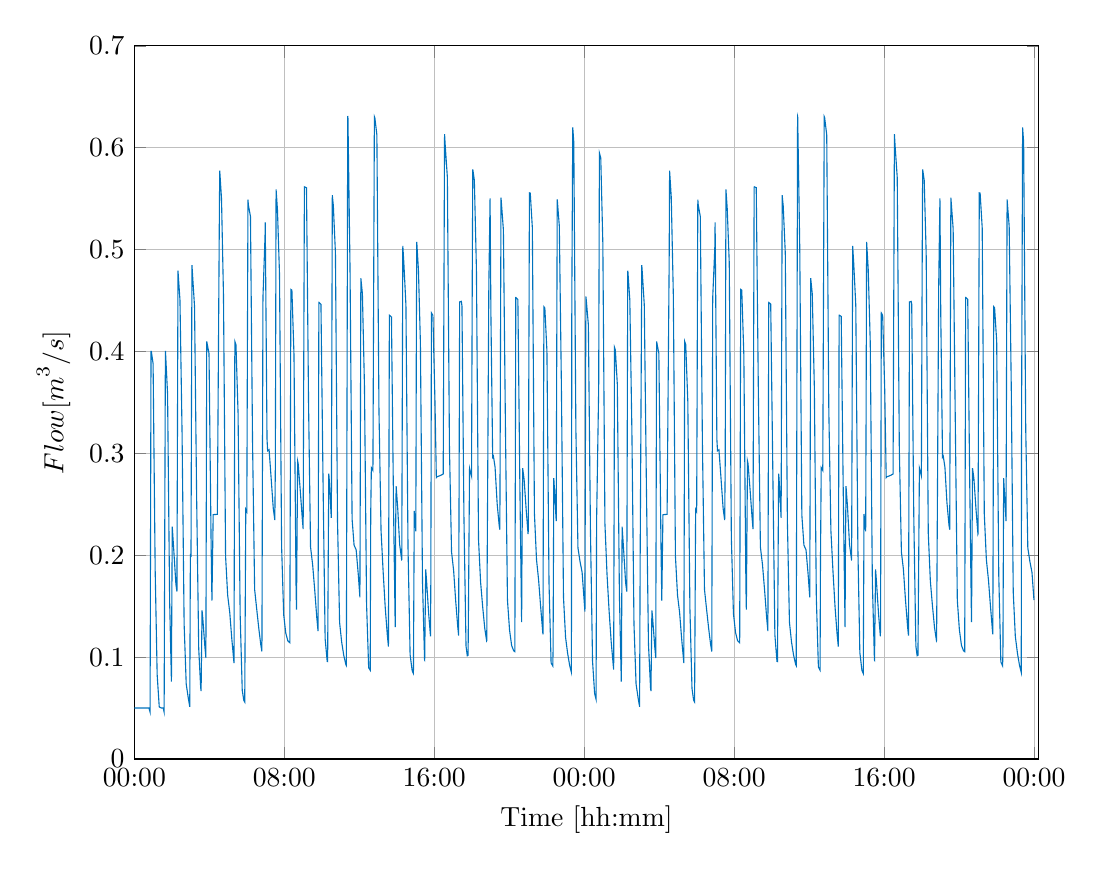
\begin{tikzpicture}

\begin{axis}[%
width=4.521in,
height=3.566in,
at={(0.758in,0.481in)},
scale only axis,
xmin=1,
scaled x ticks = false,
xmajorgrids,
ymajorgrids,
xmax=173664,
xtick={1,28801,57601,86401,115201,144001,172801},
xticklabels={{00:00},{08:00},{16:00},{00:00},{08:00},{16:00},{00:00},{},{},{}},
xlabel={Time [hh:mm]},
ymin=0,
ymax=0.7,
ylabel={$\text{Flow [m}^\text{3}\text{/s]}$},
axis background/.style={fill=white}
]
\addplot [color=mycolor1,solid,forget plot]
  table[row sep=crcr]{%
1	0.0499997152763342\\
381	0.0499999892074085\\
681	0.0499999887402718\\
781	0.0499999900942177\\
801	0.0499999900283255\\
1081	0.049999984018313\\
1261	0.0499999893262727\\
1521	0.0499999838340426\\
1601	0.049999984809447\\
2001	0.0499999906588171\\
2061	0.0499999922125646\\
2401	0.049999988996632\\
2781	0.0499999918475296\\
2801	0.0499999801986038\\
3021	0.0460373492555953\\
3201	0.39999620912548\\
3261	0.399999964024236\\
3601	0.388038894071086\\
4001	0.184947858626601\\
4381	0.082805088531536\\
4781	0.0511451879298567\\
5181	0.0500002487860619\\
5541	0.0499999248577416\\
5721	0.0460373452553259\\
5961	0.399999974821009\\
5981	0.399999971271513\\
6381	0.358516455127467\\
6781	0.154383868746348\\
7121	0.0760256189325568\\
7181	0.13826974014641\\
7281	0.228026620985396\\
7581	0.204239805785136\\
7981	0.171590440555943\\
8181	0.164315181527722\\
8381	0.47926934050765\\
8761	0.450413278243777\\
9161	0.321534576651487\\
9561	0.132277730995904\\
9961	0.0735649221955217\\
10361	0.0597071439387407\\
10641	0.0512695775424259\\
10761	0.20005447478489\\
10881	0.199434615905679\\
11061	0.48473586623314\\
11161	0.476723871738909\\
11561	0.443897750738214\\
11961	0.25806849480281\\
12361	0.108844325174995\\
12741	0.0700275093087758\\
12821	0.0667206908995504\\
13001	0.145928679109392\\
13141	0.138393729441425\\
13541	0.110667079625233\\
13741	0.0991507389943454\\
13901	0.40986305875768\\
13941	0.40882623802115\\
14341	0.398007217901318\\
14741	0.212131825065823\\
14901	0.155368306478837\\
15141	0.239872608579426\\
15541	0.240004691937102\\
15941	0.240038886655287\\
16341	0.543707035296884\\
16401	0.577386156049016\\
16741	0.5499489464615\\
17121	0.454515865313659\\
17521	0.199211784759613\\
17921	0.160813386913845\\
18321	0.143916888943139\\
18721	0.117703671201611\\
19121	0.095049498732015\\
19141	0.0940665657039142\\
19301	0.409784435964215\\
19521	0.406501876116627\\
19921	0.33935537668123\\
20321	0.141804797058712\\
20721	0.067435176520201\\
21021	0.0575846925747079\\
21201	0.0559457131457851\\
21401	0.244991184003057\\
21601	0.242763538199487\\
21821	0.5490148580277\\
21901	0.543815970276843\\
22301	0.532449053725931\\
22701	0.311242442063504\\
23101	0.166455067970211\\
23501	0.147143722635203\\
23901	0.128218569971245\\
24301	0.111515660096113\\
24501	0.105546274424128\\
24701	0.452877166239096\\
25101	0.513490813859022\\
25141	0.526641040406919\\
25481	0.314069608587414\\
25601	0.302486128983783\\
25881	0.303568709699798\\
26281	0.275044058907798\\
26681	0.245964195626756\\
26981	0.234447696691942\\
27081	0.288110624118585\\
27221	0.559006245862765\\
27481	0.539613674285018\\
27881	0.475567692570443\\
28281	0.209018911404775\\
28681	0.141668747218986\\
29081	0.123608641874535\\
29481	0.11592694443507\\
29861	0.114080220104003\\
30061	0.460896204122244\\
30261	0.460167448207798\\
30661	0.396678419054452\\
31061	0.168157104268696\\
31141	0.146550603859365\\
31361	0.292440612392119\\
31461	0.290155884720642\\
31861	0.26381450895376\\
32261	0.23554830781087\\
32421	0.225714221407563\\
32661	0.561584147546688\\
33061	0.560624758930501\\
33461	0.348105695677251\\
33841	0.208065283311125\\
34241	0.190782917669544\\
34641	0.166025134280847\\
35041	0.13873822553377\\
35281	0.125451644802619\\
35441	0.4478352243038\\
35461	0.44811407769246\\
35841	0.446214141629251\\
36241	0.27225617680166\\
36641	0.118110855826106\\
37041	0.095767561962741\\
37121	0.0956553614348974\\
37341	0.280096449864026\\
37441	0.273855912758517\\
37821	0.236596990821348\\
37841	0.237774941596493\\
38021	0.553366894967955\\
38221	0.54291518952707\\
38621	0.49660305179753\\
39021	0.233847581211315\\
39421	0.134033881707084\\
39821	0.114649017608518\\
40221	0.101701052031103\\
40621	0.0927146992547936\\
40721	0.0917383187540116\\
40981	0.63107071951054\\
41021	0.630035704702444\\
41421	0.482341851596278\\
41821	0.235563366290832\\
42201	0.209832049584584\\
42601	0.205284923234108\\
43001	0.181573721441432\\
43321	0.158651139798747\\
43401	0.287395033266756\\
43501	0.471956377710797\\
43801	0.456578916341174\\
44201	0.364798527107059\\
44601	0.151919551074707\\
45001	0.0895967214260026\\
45301	0.0871144475971674\\
45401	0.241707281322062\\
45521	0.285948268035892\\
45821	0.283146889932263\\
46101	0.630469173265171\\
46201	0.629088537957435\\
46581	0.612545920500935\\
46981	0.342528955023114\\
47381	0.224203484709649\\
47781	0.184153073081266\\
48181	0.149030782566006\\
48581	0.12195593910867\\
48801	0.110280587955104\\
48981	0.435567061037672\\
49381	0.433837256348174\\
49781	0.247137117278272\\
50101	0.129323544894529\\
50181	0.226587016813804\\
50281	0.267899772040847\\
50581	0.246318904302867\\
50961	0.210314398331763\\
51341	0.195657253277077\\
51361	0.195784009404707\\
51561	0.503592036774015\\
51761	0.486974841272141\\
52161	0.445428690023276\\
52561	0.207716541625214\\
52961	0.102502304765683\\
53361	0.0865204262570826\\
53601	0.0839471479111217\\
53761	0.243524692542883\\
54061	0.22335472358936\\
54161	0.413641605154435\\
54241	0.507566556159231\\
54561	0.48007415997152\\
54941	0.408444008474248\\
55341	0.174114153859742\\
55741	0.0971405673619263\\
55761	0.096975498915427\\
55961	0.186119510987269\\
56141	0.173353292951344\\
56541	0.141804669337536\\
56881	0.120312676919824\\
56941	0.17363089926247\\
57061	0.437782042398014\\
57341	0.435474087380637\\
57741	0.350377749978731\\
58001	0.276216298585415\\
58141	0.277039370834222\\
58541	0.277740752111343\\
58941	0.278635286488113\\
59321	0.279736664395953\\
59581	0.613239888945005\\
59721	0.601155920090224\\
60121	0.570829618399022\\
60521	0.30525522703366\\
60921	0.203256919582693\\
61321	0.185129585157137\\
61721	0.154979527639579\\
62121	0.129229876043253\\
62281	0.12114747426953\\
62481	0.44862995078268\\
62801	0.449171273418054\\
62921	0.444677955276041\\
63301	0.237964284751834\\
63701	0.111008795041031\\
63941	0.101319095647373\\
64101	0.101831871303562\\
64381	0.285451159479523\\
64761	0.277800728120848\\
64901	0.472346688429331\\
65001	0.578732309508892\\
65301	0.568128800263333\\
65701	0.480556114992309\\
66101	0.215435701651473\\
66501	0.173587977353262\\
66901	0.149411121057409\\
67301	0.128194088457934\\
67661	0.115879979337036\\
67681	0.116080976474654\\
68081	0.463231310412606\\
68321	0.550240918542084\\
68481	0.43704169328213\\
68821	0.296195131686067\\
68961	0.297296204143991\\
69281	0.286349521684829\\
69681	0.250540179409776\\
70081	0.228693231365457\\
70201	0.225059553792036\\
70421	0.550888655859785\\
70481	0.546993291279657\\
70881	0.519239767321056\\
71281	0.321893080651539\\
71661	0.155884099827311\\
72061	0.126611870338134\\
72461	0.111441871585865\\
72861	0.106140611089357\\
73081	0.105332967336101\\
73261	0.452946083990718\\
73281	0.453024300871342\\
73661	0.451074937198832\\
74061	0.26082900810748\\
74381	0.134237338321971\\
74461	0.207813944879953\\
74581	0.285378186391529\\
74861	0.274285223507388\\
75261	0.244391347849864\\
75621	0.220651866001535\\
75661	0.224809763811749\\
75881	0.5556579938168\\
76041	0.555440125466322\\
76441	0.52143634234302\\
76841	0.240745754972094\\
77241	0.195680996475161\\
77641	0.175811605109868\\
78041	0.149008733822511\\
78441	0.124162090755598\\
78481	0.122293389503727\\
78661	0.44384907080836\\
78841	0.442708151044371\\
79241	0.400372910545192\\
79641	0.172855897377427\\
80041	0.0943411879687305\\
80361	0.0913677029693039\\
80421	0.105748914607317\\
80561	0.275622277873239\\
81021	0.233525034544167\\
81221	0.549299988830962\\
81621	0.523015869588244\\
82021	0.365589134600443\\
82421	0.158832345842062\\
82821	0.119381319389791\\
83221	0.103510284822917\\
83621	0.0914259162743653\\
83941	0.0850821629137212\\
84021	0.449966203224246\\
84201	0.619938777189986\\
84401	0.605215327407337\\
84801	0.323950052106171\\
85201	0.207162769487388\\
85601	0.193722933184863\\
86001	0.183208432749678\\
86401	0.154546451194393\\
86541	0.144709226768709\\
86721	0.454054707630259\\
86801	0.450268450488853\\
87201	0.426082168190829\\
87601	0.224018825746384\\
88001	0.0961050037604321\\
88401	0.0642514476254031\\
88681	0.058588377418986\\
88781	0.233884823055304\\
89181	0.363764232190534\\
89321	0.594800267880994\\
89581	0.589951272879468\\
89981	0.505665048374919\\
90381	0.231007553197322\\
90781	0.181446768847678\\
91181	0.145374472013491\\
91581	0.115191653805948\\
91981	0.0918291899207325\\
92061	0.0877953189909785\\
92221	0.403907758239193\\
92381	0.401514711023063\\
92761	0.367814281450466\\
93161	0.161459811427181\\
93521	0.0760258697047347\\
93561	0.0969253175283628\\
93681	0.228026635800281\\
93961	0.206157068010913\\
94361	0.172716138741509\\
94581	0.164315181527722\\
94761	0.477771577804068\\
94781	0.47926934050765\\
95161	0.450413278243778\\
95561	0.321534576651487\\
95961	0.132277730995905\\
96361	0.0735649221955217\\
96761	0.0597071439387407\\
97041	0.0512695775424261\\
97141	0.189954342640788\\
97461	0.48473586623314\\
97541	0.478621526310808\\
97941	0.445565551010111\\
98341	0.270052824073967\\
98741	0.112972942133323\\
99141	0.0700275093087758\\
99221	0.0667206908995504\\
99401	0.145928679109392\\
99541	0.138393729441425\\
99941	0.110667079625233\\
100141	0.0991507389943454\\
100301	0.40986305875768\\
100341	0.40882623802115\\
100741	0.398007217901318\\
101141	0.212131825065823\\
101301	0.155368306478837\\
101521	0.239674727124832\\
101921	0.240004160488744\\
102321	0.240032761489357\\
102721	0.490613201150536\\
102801	0.577385614042946\\
103121	0.551397788492204\\
103521	0.454515521091378\\
103921	0.199211766547411\\
104321	0.160811738559319\\
104721	0.143916519077449\\
105121	0.117702397972358\\
105501	0.0960563302766093\\
105541	0.0940655608631718\\
105701	0.409782142347942\\
105901	0.406701240316587\\
106301	0.350756062230757\\
106701	0.148179236245713\\
107101	0.0692618286459731\\
107421	0.0575801460066641\\
107601	0.0559429268585551\\
107801	0.244982676605651\\
108001	0.242757068811194\\
108221	0.54900476716055\\
108301	0.543808297503321\\
108701	0.532436480925017\\
109101	0.311241030199004\\
109501	0.166447159541348\\
109881	0.14801645052783\\
110281	0.129144882903335\\
110681	0.112225593742404\\
110901	0.105541387787785\\
111081	0.452627367523953\\
111481	0.501364815585408\\
111541	0.526586805232183\\
111881	0.314064927206939\\
112001	0.302477482482032\\
112281	0.303564415396613\\
112681	0.275045931553673\\
113081	0.245964222909356\\
113381	0.234448498754518\\
113481	0.288116696094247\\
113621	0.559006398210286\\
113861	0.540979121709231\\
114261	0.486855270635058\\
114661	0.217493518570819\\
115061	0.142802563645621\\
115461	0.124291854749527\\
115861	0.116093137321325\\
116261	0.114084290390741\\
116461	0.460899377915235\\
116661	0.460171947548487\\
117061	0.396679285152434\\
117461	0.168158461755987\\
117541	0.146555138425319\\
117761	0.292445572598367\\
117861	0.290159181668251\\
118241	0.265401886805784\\
118641	0.236956301886082\\
118821	0.225714522330167\\
119041	0.561469488609575\\
119061	0.561586041554716\\
119441	0.560805439144691\\
119841	0.363932228586388\\
120241	0.208067125535311\\
120641	0.190785255682231\\
121041	0.166025588105298\\
121441	0.13873932167539\\
121681	0.125453388188775\\
121841	0.447837563995478\\
121861	0.448116051383338\\
122221	0.4464561479952\\
122621	0.284824476239217\\
123021	0.121970167931679\\
123421	0.0958081500032729\\
123521	0.0956573749864267\\
123741	0.280096851577685\\
123821	0.275531608454023\\
124221	0.236598409026601\\
124421	0.553367619300467\\
124621	0.5429157709688\\
125021	0.496603413412628\\
125421	0.233847680410384\\
125821	0.134033685469667\\
126221	0.114650333534502\\
126601	0.102289103709303\\
127001	0.0929882528747439\\
127121	0.0917392868371645\\
127381	0.631071912873843\\
127401	0.630719116657667\\
127801	0.501347161814062\\
128201	0.239397450469059\\
128601	0.209832888971714\\
129001	0.205285541414406\\
129401	0.181574246023112\\
129721	0.158651581187078\\
129801	0.287397627582394\\
129901	0.471956617871342\\
130201	0.456579492165227\\
130601	0.364798643465493\\
130981	0.158461721428025\\
131381	0.0902446213392131\\
131701	0.0871147730920042\\
131781	0.195332180975037\\
131921	0.285946978271874\\
132221	0.283146011645084\\
132501	0.630469563534361\\
132581	0.62947257325151\\
132981	0.612546279103266\\
133381	0.342529069488647\\
133781	0.22420331583186\\
134181	0.18415338411579\\
134581	0.149030236035514\\
134961	0.123132349572876\\
135201	0.110280603793395\\
135361	0.435176913377614\\
135381	0.435567198316332\\
135761	0.434402963450522\\
136161	0.258663077151003\\
136501	0.129324848709165\\
136561	0.193972315730123\\
136681	0.267900152487372\\
136961	0.248282666486158\\
137361	0.210314788420516\\
137741	0.195657673398787\\
137761	0.195784442440667\\
137961	0.503592296507298\\
138161	0.48697576182077\\
138561	0.445428205217198\\
138961	0.207716601935443\\
139341	0.104535524709347\\
139741	0.0868948301247878\\
140001	0.0839475146696737\\
140141	0.240432040289202\\
140461	0.223354613707161\\
140541	0.341067258228241\\
140641	0.507566355305644\\
140941	0.481669135095204\\
141341	0.408443854052323\\
141741	0.174114080843233\\
142141	0.0971401552400959\\
142161	0.0969748967063283\\
142361	0.186118838354968\\
142541	0.173352807110823\\
142941	0.141804218930691\\
143281	0.120311786985649\\
143321	0.129127350722078\\
143461	0.437780930522792\\
143721	0.435517651687087\\
144121	0.361960854279469\\
144401	0.276209489946611\\
144521	0.277012003580165\\
144921	0.277695129632075\\
145321	0.278586129391934\\
145721	0.279729241245801\\
145981	0.613237806000591\\
146121	0.601153312486374\\
146521	0.570827166257067\\
146921	0.305254463448292\\
147321	0.20325470575301\\
147701	0.186543247083285\\
148101	0.15643029351033\\
148501	0.130357894127212\\
148681	0.121144762304623\\
148881	0.448629034177187\\
149201	0.449165808875287\\
149301	0.446696179355606\\
149701	0.237965618956237\\
150101	0.111008331346555\\
150341	0.101316327092596\\
150501	0.101826939135492\\
150781	0.285447611650934\\
151161	0.27779589570848\\
151301	0.472339570784934\\
151401	0.578729951396445\\
151701	0.568123276721063\\
152081	0.495832401738009\\
152481	0.221821174469093\\
152881	0.17473208468221\\
153281	0.150604920464296\\
153681	0.12910065597234\\
154061	0.115878791323534\\
154081	0.116079655938807\\
154481	0.463229573529833\\
154721	0.5502375854001\\
154881	0.437041948039623\\
155221	0.296195355930144\\
155361	0.297296933741909\\
155681	0.286350503920018\\
156061	0.252102910380496\\
156461	0.229497997298456\\
156601	0.225064130916765\\
156821	0.550890260513285\\
156861	0.548562055547551\\
157261	0.520520415207785\\
157661	0.336720865555416\\
158061	0.155883549287124\\
158461	0.126615126562859\\
158861	0.111443479804903\\
159261	0.106144927681463\\
159481	0.105335017541325\\
159661	0.452949294313543\\
159681	0.453027104859375\\
160061	0.451077022810141\\
160441	0.272986614049946\\
160781	0.134240624188618\\
160841	0.171194243932062\\
160981	0.285380797796743\\
161241	0.27560958645801\\
161641	0.245748272441495\\
162021	0.22065246306675\\
162041	0.22095872866312\\
162281	0.555659486202346\\
162441	0.555441569380212\\
162841	0.521436911503331\\
163241	0.240744945577966\\
163641	0.195682416129531\\
164041	0.175812474037148\\
164421	0.150374209915759\\
164821	0.125268272587349\\
164881	0.122293793898792\\
165061	0.443850629799895\\
165221	0.442791980296207\\
165621	0.41026583231508\\
166021	0.18061579852657\\
166421	0.0952920563520666\\
166761	0.09137016735018\\
166821	0.105761024965842\\
166961	0.275625277048089\\
167421	0.233525909462804\\
167621	0.549302071760907\\
168021	0.523017665432503\\
168421	0.365587501813481\\
168801	0.163841775577553\\
169201	0.120372383531068\\
169601	0.10417680851964\\
170001	0.0919608721649096\\
170341	0.0850844928164687\\
170401	0.33174516873495\\
170601	0.619937197264595\\
170801	0.605220107773325\\
171201	0.323949146474474\\
171601	0.207163720135008\\
172001	0.193730162139822\\
172401	0.183213876546389\\
172781	0.156061090616425\\
};
\end{axis}
\end{tikzpicture}%
	%\caption{Output of the last pipe into the WWTP.}
	\label{fig:Simulering_output_first}
	\end{figure}  
	\vspace{-9mm}   
	\begin{figure}
	\centering
	% This file was created by matlab2tikz.
%
%The latest updates can be retrieved from
%  http://www.mathworks.com/matlabcentral/fileexchange/22022-matlab2tikz-matlab2tikz
%where you can also make suggestions and rate matlab2tikz.
%
\definecolor{mycolor1}{rgb}{0.00000,0.44700,0.74100}%
%
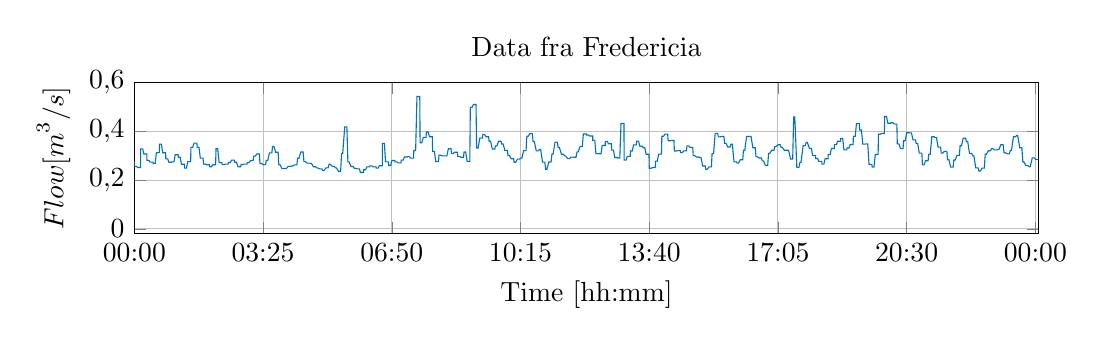
\begin{tikzpicture}

\begin{axis}[%
width=4.521in,
/pgf/number format/1000 sep={.},/pgf/number format/use comma,
height=.7566in,
scaled x ticks = false,
at={(0.758in,0.481in)},
title={Data fra Fredericia},
scale only axis,
xmin=10081,
xmax=27362,
xtick={10081,12541,15001,17461,19921,22381,24841,27301},
xticklabels={{00:00},{03:25},{06:50},{10:15},{13:40},{17:05},{20:30},{00:00},{},{}},
xlabel={Time [hh:mm]},
xmajorgrids,
ymin=-0.02,
ymax=0.6,
ylabel={$\text{Flow [m}^\text{3}\text{/s]}$},
ymajorgrids,
axis background/.style={fill=white}
]
\addplot [color=mycolor1,solid,forget plot]
  table[row sep=crcr]{%
10081	0.276666666666667\\
10082	0.256111111111111\\
10121	0.256111111111111\\
10142	0.251944444444444\\
10161	0.251944444444444\\
10201	0.251944444444444\\
10202	0.327777777777778\\
10241	0.327777777777778\\
10262	0.306944444444444\\
10281	0.306944444444444\\
10320	0.306944444444444\\
10322	0.280833333333333\\
10360	0.280833333333333\\
10382	0.273888888888889\\
10400	0.273888888888889\\
10440	0.273888888888889\\
10442	0.268055555555556\\
10480	0.268055555555556\\
10502	0.312777777777778\\
10519	0.312777777777778\\
10559	0.312777777777778\\
10562	0.3475\\
10599	0.3475\\
10622	0.312222222222222\\
10639	0.312222222222222\\
10679	0.312222222222222\\
10682	0.286944444444444\\
10719	0.286944444444444\\
10742	0.273333333333333\\
10758	0.273333333333333\\
10798	0.273333333333333\\
10802	0.274722222222222\\
10838	0.274722222222222\\
10862	0.304166666666667\\
10878	0.304166666666667\\
10918	0.304166666666667\\
10922	0.293888888888889\\
10957	0.293888888888889\\
10982	0.265\\
10997	0.265\\
11037	0.265\\
11042	0.249166666666667\\
11077	0.249166666666667\\
11102	0.275555555555556\\
11117	0.275555555555556\\
11157	0.275555555555556\\
11162	0.334166666666667\\
11196	0.334166666666667\\
11222	0.351666666666667\\
11236	0.351666666666667\\
11276	0.351666666666667\\
11282	0.334166666666667\\
11316	0.334166666666667\\
11342	0.29\\
11356	0.29\\
11395	0.29\\
11402	0.266111111111111\\
11435	0.266111111111111\\
11462	0.263055555555556\\
11475	0.263055555555556\\
11515	0.263055555555556\\
11522	0.255\\
11555	0.255\\
11582	0.263055555555556\\
11594	0.263055555555556\\
11634	0.263055555555556\\
11642	0.328611111111111\\
11674	0.328611111111111\\
11702	0.271666666666667\\
11714	0.271666666666667\\
11754	0.271666666666667\\
11762	0.263333333333333\\
11794	0.263333333333333\\
11822	0.265833333333333\\
11833	0.265833333333333\\
11873	0.265833333333333\\
11882	0.272222222222222\\
11913	0.272222222222222\\
11942	0.281944444444444\\
11953	0.281944444444444\\
11993	0.281944444444444\\
12002	0.273055555555556\\
12032	0.273055555555556\\
12062	0.254722222222222\\
12072	0.254722222222222\\
12112	0.254722222222222\\
12122	0.264166666666667\\
12152	0.264166666666667\\
12182	0.265833333333333\\
12192	0.265833333333333\\
12232	0.265833333333333\\
12242	0.271944444444444\\
12271	0.271944444444444\\
12302	0.279722222222222\\
12311	0.279722222222222\\
12351	0.279722222222222\\
12362	0.298333333333333\\
12391	0.298333333333333\\
12422	0.306944444444444\\
12431	0.306944444444444\\
12470	0.306944444444444\\
12482	0.268333333333333\\
12510	0.268333333333333\\
12542	0.263611111111111\\
12550	0.263611111111111\\
12590	0.263611111111111\\
12602	0.280555555555556\\
12630	0.280555555555556\\
12662	0.311666666666667\\
12670	0.311666666666667\\
12709	0.311666666666667\\
12722	0.338333333333333\\
12749	0.338333333333333\\
12782	0.314166666666667\\
12789	0.314166666666667\\
12829	0.314166666666667\\
12842	0.262222222222222\\
12869	0.262222222222222\\
12902	0.246944444444444\\
12908	0.246944444444444\\
12948	0.246944444444444\\
12962	0.247777777777778\\
12988	0.247777777777778\\
13022	0.256111111111111\\
13028	0.256111111111111\\
13068	0.256111111111111\\
13082	0.258055555555556\\
13107	0.258055555555556\\
13142	0.262222222222222\\
13147	0.262222222222222\\
13187	0.262222222222222\\
13202	0.289444444444444\\
13227	0.289444444444444\\
13262	0.315277777777778\\
13267	0.315277777777778\\
13307	0.315277777777778\\
13322	0.275555555555556\\
13346	0.275555555555556\\
13382	0.269722222222222\\
13386	0.269722222222222\\
13426	0.269722222222222\\
13442	0.268611111111111\\
13466	0.268611111111111\\
13502	0.255\\
13506	0.255\\
13545	0.255\\
13562	0.25\\
13585	0.25\\
13622	0.246111111111111\\
13625	0.246111111111111\\
13665	0.246111111111111\\
13682	0.239444444444444\\
13705	0.239444444444444\\
13742	0.250277777777778\\
13745	0.250277777777778\\
13784	0.250277777777778\\
13802	0.265\\
13824	0.265\\
13862	0.256388888888889\\
13864	0.256388888888889\\
13904	0.256388888888889\\
13922	0.25\\
13944	0.25\\
13982	0.236388888888889\\
13983	0.236388888888889\\
14023	0.236388888888889\\
14042	0.309444444444444\\
14063	0.309444444444444\\
14102	0.418055555555556\\
14103	0.418055555555556\\
14143	0.418055555555556\\
14162	0.275\\
14183	0.275\\
14222	0.255833333333333\\
14262	0.255833333333333\\
14282	0.248611111111111\\
14302	0.248611111111111\\
14342	0.246111111111111\\
14382	0.246111111111111\\
14402	0.231111111111111\\
14421	0.231111111111111\\
14461	0.231111111111111\\
14462	0.2425\\
14501	0.2425\\
14522	0.254166666666667\\
14541	0.254166666666667\\
14581	0.254166666666667\\
14582	0.258611111111111\\
14620	0.258611111111111\\
14642	0.254166666666667\\
14660	0.254166666666667\\
14700	0.254166666666667\\
14702	0.249444444444444\\
14740	0.249444444444444\\
14762	0.258888888888889\\
14780	0.258888888888889\\
14820	0.258888888888889\\
14822	0.350833333333333\\
14859	0.350833333333333\\
14882	0.275\\
14899	0.275\\
14939	0.275\\
14942	0.26\\
14979	0.26\\
15002	0.280277777777778\\
15019	0.280277777777778\\
15058	0.280277777777778\\
15062	0.274722222222222\\
15098	0.274722222222222\\
15122	0.270555555555556\\
15138	0.270555555555556\\
15178	0.270555555555556\\
15182	0.281666666666667\\
15218	0.281666666666667\\
15242	0.294722222222222\\
15258	0.294722222222222\\
15297	0.294722222222222\\
15302	0.296111111111111\\
15337	0.296111111111111\\
15362	0.29\\
15377	0.29\\
15417	0.29\\
15422	0.321388888888889\\
15457	0.321388888888889\\
15482	0.542777777777778\\
15496	0.542777777777778\\
15536	0.542777777777778\\
15542	0.353333333333333\\
15576	0.353333333333333\\
15602	0.375\\
15616	0.375\\
15656	0.375\\
15662	0.397222222222222\\
15696	0.397222222222222\\
15722	0.377777777777778\\
15735	0.377777777777778\\
15775	0.377777777777778\\
15782	0.317777777777778\\
15815	0.317777777777778\\
15842	0.276111111111111\\
15855	0.276111111111111\\
15895	0.276111111111111\\
15902	0.301944444444444\\
15934	0.301944444444444\\
15962	0.299444444444444\\
15974	0.299444444444444\\
16014	0.299444444444444\\
16054	0.299444444444444\\
16082	0.328333333333333\\
16094	0.328333333333333\\
16133	0.328333333333333\\
16142	0.309444444444444\\
16173	0.309444444444444\\
16202	0.314166666666667\\
16213	0.314166666666667\\
16253	0.314166666666667\\
16262	0.2975\\
16293	0.2975\\
16322	0.293888888888889\\
16333	0.293888888888889\\
16372	0.293888888888889\\
16382	0.315277777777778\\
16412	0.315277777777778\\
16442	0.276666666666667\\
16452	0.276666666666667\\
16492	0.276666666666667\\
16502	0.4975\\
16532	0.4975\\
16562	0.510277777777778\\
16571	0.510277777777778\\
16611	0.510277777777778\\
16622	0.331666666666667\\
16651	0.331666666666667\\
16682	0.371944444444444\\
16691	0.371944444444444\\
16731	0.371944444444444\\
16742	0.3875\\
16771	0.3875\\
16802	0.377777777777778\\
16810	0.377777777777778\\
16850	0.377777777777778\\
16862	0.359166666666667\\
16890	0.359166666666667\\
16922	0.3275\\
16930	0.3275\\
16970	0.3275\\
16982	0.34\\
17009	0.34\\
17042	0.359166666666667\\
17049	0.359166666666667\\
17089	0.359166666666667\\
17102	0.348055555555556\\
17129	0.348055555555556\\
17162	0.321666666666667\\
17169	0.321666666666667\\
17209	0.321666666666667\\
17222	0.301388888888889\\
17248	0.301388888888889\\
17282	0.2875\\
17288	0.2875\\
17328	0.2875\\
17342	0.273055555555556\\
17368	0.273055555555556\\
17402	0.286111111111111\\
17408	0.286111111111111\\
17447	0.286111111111111\\
17462	0.290277777777778\\
17487	0.290277777777778\\
17522	0.321111111111111\\
17527	0.321111111111111\\
17567	0.321111111111111\\
17582	0.379722222222222\\
17607	0.379722222222222\\
17642	0.390277777777778\\
17646	0.390277777777778\\
17686	0.390277777777778\\
17702	0.3575\\
17726	0.3575\\
17762	0.32\\
17766	0.32\\
17806	0.32\\
17822	0.325555555555556\\
17846	0.325555555555556\\
17882	0.273611111111111\\
17885	0.273611111111111\\
17925	0.273611111111111\\
17942	0.244722222222222\\
17965	0.244722222222222\\
18002	0.274166666666667\\
18005	0.274166666666667\\
18045	0.274166666666667\\
18062	0.306944444444444\\
18084	0.306944444444444\\
18122	0.355833333333333\\
18124	0.355833333333333\\
18164	0.355833333333333\\
18182	0.334166666666667\\
18204	0.334166666666667\\
18242	0.306111111111111\\
18244	0.306111111111111\\
18284	0.306111111111111\\
18302	0.299166666666667\\
18323	0.299166666666667\\
18362	0.288055555555556\\
18363	0.288055555555556\\
18403	0.288055555555556\\
18422	0.294444444444444\\
18443	0.294444444444444\\
18482	0.293888888888889\\
18483	0.293888888888889\\
18522	0.293888888888889\\
18542	0.315555555555556\\
18562	0.315555555555556\\
18602	0.338333333333333\\
18642	0.338333333333333\\
18662	0.388888888888889\\
18682	0.388888888888889\\
18721	0.388888888888889\\
18722	0.385\\
18761	0.385\\
18782	0.380833333333333\\
18801	0.380833333333333\\
18841	0.380833333333333\\
18842	0.363055555555556\\
18881	0.363055555555556\\
18902	0.308611111111111\\
18921	0.308611111111111\\
18960	0.308611111111111\\
18962	0.308055555555556\\
19000	0.308055555555556\\
19022	0.341666666666667\\
19040	0.341666666666667\\
19080	0.341666666666667\\
19082	0.358888888888889\\
19120	0.358888888888889\\
19142	0.349166666666667\\
19159	0.349166666666667\\
19199	0.349166666666667\\
19202	0.322777777777778\\
19239	0.322777777777778\\
19262	0.292777777777778\\
19279	0.292777777777778\\
19319	0.292777777777778\\
19322	0.290555555555556\\
19359	0.290555555555556\\
19382	0.4325\\
19398	0.4325\\
19438	0.4325\\
19442	0.281666666666667\\
19478	0.281666666666667\\
19502	0.2975\\
19518	0.2975\\
19558	0.2975\\
19562	0.319444444444444\\
19597	0.319444444444444\\
19622	0.344444444444444\\
19637	0.344444444444444\\
19677	0.344444444444444\\
19682	0.36\\
19717	0.36\\
19742	0.338888888888889\\
19757	0.338888888888889\\
19797	0.338888888888889\\
19802	0.3325\\
19836	0.3325\\
19862	0.306111111111111\\
19876	0.306111111111111\\
19916	0.306111111111111\\
19922	0.248611111111111\\
19956	0.248611111111111\\
19982	0.251111111111111\\
19996	0.251111111111111\\
20035	0.251111111111111\\
20042	0.277777777777778\\
20075	0.277777777777778\\
20102	0.306388888888889\\
20115	0.306388888888889\\
20155	0.306388888888889\\
20162	0.379722222222222\\
20195	0.379722222222222\\
20222	0.388611111111111\\
20234	0.388611111111111\\
20274	0.388611111111111\\
20282	0.361111111111111\\
20314	0.361111111111111\\
20342	0.3625\\
20354	0.3625\\
20394	0.3625\\
20402	0.319444444444444\\
20434	0.319444444444444\\
20462	0.320833333333333\\
20473	0.320833333333333\\
20513	0.320833333333333\\
20522	0.3125\\
20553	0.3125\\
20582	0.32\\
20593	0.32\\
20633	0.32\\
20642	0.340277777777778\\
20672	0.340277777777778\\
20702	0.334444444444444\\
20712	0.334444444444444\\
20752	0.334444444444444\\
20762	0.300277777777778\\
20792	0.300277777777778\\
20822	0.294722222222222\\
20832	0.294722222222222\\
20872	0.294722222222222\\
20882	0.292777777777778\\
20911	0.292777777777778\\
20942	0.257777777777778\\
20951	0.257777777777778\\
20991	0.257777777777778\\
21002	0.244444444444444\\
21031	0.244444444444444\\
21062	0.254166666666667\\
21071	0.254166666666667\\
21110	0.254166666666667\\
21122	0.308611111111111\\
21150	0.308611111111111\\
21182	0.391388888888889\\
21190	0.391388888888889\\
21230	0.391388888888889\\
21242	0.377222222222222\\
21270	0.377222222222222\\
21302	0.378611111111111\\
21310	0.378611111111111\\
21349	0.378611111111111\\
21362	0.350833333333333\\
21389	0.350833333333333\\
21422	0.335833333333333\\
21429	0.335833333333333\\
21469	0.335833333333333\\
21482	0.347222222222222\\
21509	0.347222222222222\\
21542	0.275\\
21548	0.275\\
21588	0.275\\
21602	0.27\\
21628	0.27\\
21662	0.283333333333333\\
21668	0.283333333333333\\
21708	0.283333333333333\\
21722	0.322222222222222\\
21747	0.322222222222222\\
21782	0.379166666666667\\
21787	0.379166666666667\\
21827	0.379166666666667\\
21842	0.378611111111111\\
21867	0.378611111111111\\
21902	0.3325\\
21907	0.3325\\
21947	0.3325\\
21962	0.296111111111111\\
21986	0.296111111111111\\
22022	0.290555555555556\\
22026	0.290555555555556\\
22066	0.290555555555556\\
22082	0.278611111111111\\
22106	0.278611111111111\\
22142	0.259444444444444\\
22146	0.259444444444444\\
22185	0.259444444444444\\
22202	0.309722222222222\\
22225	0.309722222222222\\
22262	0.322222222222222\\
22265	0.322222222222222\\
22305	0.322222222222222\\
22322	0.337777777777778\\
22345	0.337777777777778\\
22382	0.345\\
22385	0.345\\
22424	0.345\\
22442	0.334444444444444\\
22464	0.334444444444444\\
22502	0.3225\\
22504	0.3225\\
22544	0.3225\\
22584	0.3225\\
22622	0.286388888888889\\
22623	0.286388888888889\\
22663	0.286388888888889\\
22682	0.459166666666667\\
22703	0.459166666666667\\
22742	0.2525\\
22743	0.2525\\
22783	0.2525\\
22802	0.273333333333333\\
22823	0.273333333333333\\
22862	0.341111111111111\\
22902	0.341111111111111\\
22922	0.354722222222222\\
22942	0.354722222222222\\
22982	0.330277777777778\\
23022	0.330277777777778\\
23042	0.301111111111111\\
23061	0.301111111111111\\
23101	0.301111111111111\\
23102	0.288611111111111\\
23141	0.288611111111111\\
23162	0.276666666666667\\
23181	0.276666666666667\\
23221	0.276666666666667\\
23222	0.265277777777778\\
23260	0.265277777777778\\
23282	0.2875\\
23300	0.2875\\
23340	0.2875\\
23342	0.305\\
23380	0.305\\
23402	0.329444444444444\\
23420	0.329444444444444\\
23460	0.329444444444444\\
23462	0.345555555555556\\
23499	0.345555555555556\\
23522	0.359166666666667\\
23539	0.359166666666667\\
23579	0.359166666666667\\
23582	0.370833333333333\\
23619	0.370833333333333\\
23642	0.324166666666667\\
23659	0.324166666666667\\
23698	0.324166666666667\\
23702	0.331666666666667\\
23738	0.331666666666667\\
23762	0.345833333333333\\
23778	0.345833333333333\\
23818	0.345833333333333\\
23822	0.379444444444444\\
23858	0.379444444444444\\
23882	0.431388888888889\\
23898	0.431388888888889\\
23937	0.431388888888889\\
23942	0.405277777777778\\
23977	0.405277777777778\\
24002	0.347777777777778\\
24017	0.347777777777778\\
24057	0.347777777777778\\
24062	0.348333333333333\\
24097	0.348333333333333\\
24122	0.264722222222222\\
24136	0.264722222222222\\
24176	0.264722222222222\\
24182	0.253055555555556\\
24216	0.253055555555556\\
24242	0.305\\
24256	0.305\\
24296	0.305\\
24302	0.388055555555556\\
24336	0.388055555555556\\
24362	0.390833333333333\\
24375	0.390833333333333\\
24415	0.390833333333333\\
24422	0.461111111111111\\
24455	0.461111111111111\\
24482	0.433055555555556\\
24495	0.433055555555556\\
24535	0.433055555555556\\
24542	0.435277777777778\\
24574	0.435277777777778\\
24602	0.429722222222222\\
24614	0.429722222222222\\
24654	0.429722222222222\\
24662	0.348333333333333\\
24694	0.348333333333333\\
24722	0.329166666666667\\
24734	0.329166666666667\\
24773	0.329166666666667\\
24782	0.361388888888889\\
24813	0.361388888888889\\
24842	0.394166666666667\\
24853	0.394166666666667\\
24893	0.394166666666667\\
24902	0.393611111111111\\
24933	0.393611111111111\\
24962	0.365\\
24973	0.365\\
25012	0.365\\
25022	0.350277777777778\\
25052	0.350277777777778\\
25082	0.310833333333333\\
25092	0.310833333333333\\
25132	0.310833333333333\\
25142	0.2625\\
25172	0.2625\\
25202	0.279444444444444\\
25211	0.279444444444444\\
25251	0.279444444444444\\
25262	0.305555555555556\\
25291	0.305555555555556\\
25322	0.3775\\
25331	0.3775\\
25371	0.3775\\
25382	0.373888888888889\\
25411	0.373888888888889\\
25442	0.335277777777778\\
25450	0.335277777777778\\
25490	0.335277777777778\\
25502	0.310833333333333\\
25530	0.310833333333333\\
25562	0.318055555555556\\
25570	0.318055555555556\\
25610	0.318055555555556\\
25622	0.283333333333333\\
25649	0.283333333333333\\
25682	0.253333333333333\\
25689	0.253333333333333\\
25729	0.253333333333333\\
25742	0.2825\\
25769	0.2825\\
25802	0.301666666666667\\
25809	0.301666666666667\\
25849	0.301666666666667\\
25862	0.340833333333333\\
25888	0.340833333333333\\
25922	0.371666666666667\\
25928	0.371666666666667\\
25968	0.371666666666667\\
25982	0.358055555555556\\
26008	0.358055555555556\\
26042	0.309722222222222\\
26048	0.309722222222222\\
26087	0.309722222222222\\
26102	0.299444444444444\\
26127	0.299444444444444\\
26162	0.25\\
26167	0.25\\
26207	0.25\\
26222	0.2375\\
26247	0.2375\\
26282	0.249166666666667\\
26286	0.249166666666667\\
26326	0.249166666666667\\
26342	0.305833333333333\\
26366	0.305833333333333\\
26402	0.320555555555556\\
26406	0.320555555555556\\
26446	0.320555555555556\\
26462	0.328888888888889\\
26486	0.328888888888889\\
26522	0.323888888888889\\
26525	0.323888888888889\\
26565	0.323888888888889\\
26582	0.325833333333333\\
26605	0.325833333333333\\
26642	0.345555555555556\\
26645	0.345555555555556\\
26685	0.345555555555556\\
26702	0.312222222222222\\
26724	0.312222222222222\\
26762	0.307777777777778\\
26764	0.307777777777778\\
26804	0.307777777777778\\
26822	0.321388888888889\\
26844	0.321388888888889\\
26882	0.3775\\
26884	0.3775\\
26924	0.3775\\
26942	0.382777777777778\\
26963	0.382777777777778\\
27002	0.332777777777778\\
27003	0.332777777777778\\
27043	0.332777777777778\\
27062	0.274166666666667\\
27083	0.274166666666667\\
27122	0.259166666666667\\
27123	0.259166666666667\\
27162	0.259166666666667\\
27182	0.254444444444444\\
27202	0.254444444444444\\
27242	0.291388888888889\\
27282	0.291388888888889\\
27302	0.285277777777778\\
27361	0.285277777777778\\
};
\end{axis}
\end{tikzpicture}%
	%\caption{Simulering of COD output of the last pipe into the WWTP.}
	\label{fig:Simulering_outwqeqwesadput_first_concentration}
	\end{figure} 
	\vfill \vfill
\end{frame}

\begin{frame}{Resultat}{Test}
    
	\vfill \vfill \centering
	\begin{figure}
	\centering
	% This file was created by matlab2tikz.
%
%The latest updates can be retrieved from
%  http://www.mathworks.com/matlabcentral/fileexchange/22022-matlab2tikz-matlab2tikz
%where you can also make suggestions and rate matlab2tikz.
%
\definecolor{mycolor1}{rgb}{0.00000,0.44700,0.74100}%
%
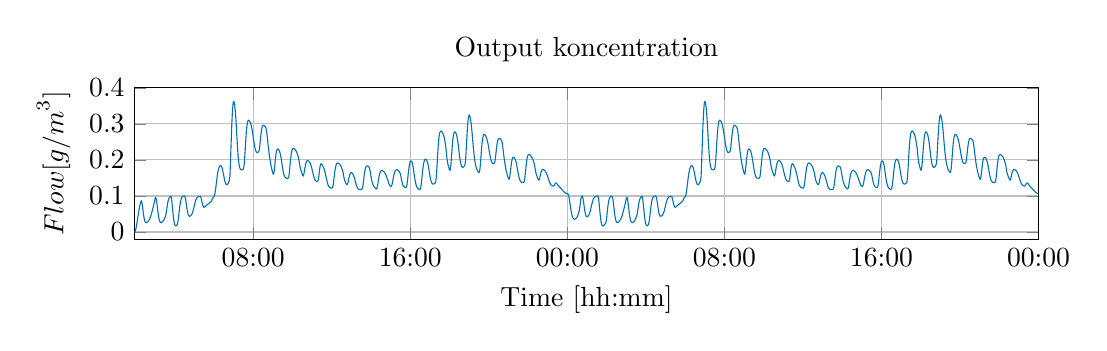
\begin{tikzpicture}

\begin{axis}[%
width=4.521in,
height=.7566in,
at={(2.6in,1.103in)},
scale only axis,
xmin=7000,
xmax=172801,
scaled x ticks = false,
xtick={1,28801,57601,86401,115201,144001,172801},
xticklabels={{00:00},{08:00},{16:00},{00:00},{08:00},{16:00},{00:00},{},{},{}},
xlabel={Time [hh:mm]},
xmajorgrids,
ymin=-0.02,
title={Output koncentration},
ymax=0.4,
ylabel={$\text{Flow [g/m}^\text{3}\text{]}$},
ymajorgrids,
axis background/.style={fill=white}
]
\addplot [color=mycolor1,solid,forget plot]
  table[row sep=crcr]{%
1	0\\
121	2.76444442474818e-109\\
241	3.26073009656065e-101\\
361	1.48722057706843e-94\\
481	9.07390854028621e-89\\
601	1.30076980586151e-83\\
701	1.08231091808059e-79\\
821	2.34738673163703e-75\\
941	1.3221333746199e-71\\
1061	3.20198537091244e-68\\
1181	5.82305692307098e-65\\
1281	2.4454529018171e-62\\
1401	2.56257479015984e-59\\
1521	1.86758071874072e-56\\
1641	9.43803249298235e-54\\
1761	3.39269645825311e-51\\
1861	3.59818145508685e-49\\
1981	7.43145424886407e-47\\
2101	1.16307577120233e-44\\
2221	1.36721652521903e-42\\
2341	1.68660368903054e-40\\
2441	2.35170957410801e-38\\
2561	1.30216127876707e-35\\
2681	5.85644996006396e-33\\
2801	2.24306122131333e-30\\
2921	7.60106686999932e-28\\
3021	9.43709554482937e-26\\
3141	5.90013951008352e-24\\
3261	1.46846532824227e-22\\
3381	2.2857813314748e-21\\
3501	1.97863169905587e-20\\
3601	7.73043630786215e-20\\
3721	2.56726045688387e-19\\
3841	6.26014920021868e-19\\
3961	1.31614841955074e-18\\
4081	2.72131669579753e-18\\
4201	6.30987738515826e-18\\
4301	1.51616521416971e-17\\
4421	5.60851788410215e-17\\
4541	2.6339333933766e-16\\
4661	1.44015306390873e-15\\
4781	8.3680115338951e-15\\
4881	3.58922621658711e-14\\
5001	1.95645240511166e-13\\
5121	9.94480128372167e-13\\
5241	4.70720404733287e-12\\
5361	2.09076018752307e-11\\
5461	7.41644489455555e-11\\
5581	7.24214793184579e-10\\
5701	3.19707992924011e-08\\
5821	5.70608545570831e-07\\
5941	1.80415957151033e-06\\
6041	3.81554329006679e-06\\
6161	8.96025772167814e-06\\
6281	2.05370658114337e-05\\
6401	4.18604942471306e-05\\
6521	7.2710127704623e-05\\
6621	0.000104304049087269\\
6741	0.000148111320476602\\
6861	0.000200586684032383\\
6981	0.000293352401992236\\
7101	0.000803797805528758\\
7201	0.00373316427553855\\
7321	0.0112988676031603\\
7441	0.0216265958635804\\
7561	0.0335097595848744\\
7681	0.0456943510219533\\
7801	0.0571866413478213\\
7901	0.0657777879623588\\
8021	0.0746358522261538\\
8141	0.0817601962521725\\
8261	0.0863572379239651\\
8281	0.0865351944787299\\
8381	0.0826868352217583\\
8481	0.0729328729720781\\
8601	0.0581850217639591\\
8721	0.044725357603887\\
8841	0.0349653661350658\\
8961	0.0291117635460206\\
9061	0.0266879469917678\\
9181	0.0258176888199261\\
9301	0.0263465314669768\\
9421	0.0277559180191354\\
9541	0.0297924228569586\\
9641	0.0319095831763245\\
9761	0.0350096550170574\\
9881	0.0388979610481673\\
10001	0.0437850540515898\\
10121	0.0497235509226516\\
10221	0.0553393938893703\\
10341	0.0625459979732243\\
10461	0.0698120774104384\\
10581	0.0767734203868196\\
10701	0.0856814291484519\\
10801	0.0926672708924115\\
10921	0.0958384827779321\\
11041	0.0900904191980293\\
11161	0.0769023939612189\\
11281	0.0611460041273074\\
11401	0.0469646731364804\\
11501	0.0380020148584435\\
11621	0.0309441692446212\\
11741	0.0273062648604276\\
11861	0.0261019009205255\\
11881	0.0260683183108994\\
11981	0.0264142750430167\\
12081	0.0274151105189277\\
12201	0.0292408712994812\\
12321	0.0316333360010084\\
12441	0.0346201085339089\\
12561	0.0383691355726851\\
12661	0.0422572667088365\\
12781	0.0482707642453505\\
12901	0.0586878405116733\\
13021	0.0720749340657065\\
13141	0.0827154885680492\\
13241	0.0890266252514835\\
13361	0.0939938169869922\\
13481	0.0968879064001237\\
13601	0.0984353528010755\\
13681	0.098813076786567\\
13721	0.0985348075014154\\
13821	0.0920427152472036\\
13941	0.075298872422749\\
14061	0.0558640981645994\\
14181	0.0387744884664413\\
14301	0.0267587617468617\\
14401	0.0208505283618553\\
14521	0.0176859050948064\\
14601	0.0171756347194794\\
14641	0.0172450864809872\\
14761	0.0184330083529576\\
14881	0.021446006624673\\
15001	0.0296915590538805\\
15101	0.0411250864689163\\
15221	0.0570253559853099\\
15341	0.0720784400230032\\
15461	0.0838664180283296\\
15581	0.0916844984904187\\
15681	0.0955974324496832\\
15801	0.0981331548392821\\
15921	0.0992804902052318\\
16041	0.0997381701301001\\
16121	0.0998281957990698\\
16161	0.0997895878738131\\
16261	0.0987248170524495\\
16381	0.0922400150811175\\
16501	0.0807971195713268\\
16621	0.0676300350816622\\
16741	0.0563839869388142\\
16841	0.0498732752106481\\
16961	0.0454520402678986\\
17081	0.043803653695271\\
17121	0.0436862670521838\\
17201	0.0439124307957137\\
17321	0.0451172938670885\\
17421	0.0467706947342416\\
17541	0.0496130963654136\\
17661	0.0537529616926854\\
17781	0.0595329505449419\\
17901	0.0667566967582858\\
18001	0.0732942416336339\\
18121	0.0808092376522041\\
18241	0.0871209626258829\\
18361	0.0918274376970769\\
18481	0.0949946886522725\\
18601	0.096941432295222\\
18701	0.0979007717822553\\
18821	0.0985342103493651\\
18941	0.0988213011868767\\
19021	0.0988838206502504\\
19061	0.0988634962711278\\
19181	0.0973930870815826\\
19281	0.091820003039776\\
19401	0.0832884205445895\\
19521	0.0755208977191211\\
19641	0.0705093124587236\\
19761	0.0686969434456523\\
19781	0.0686581463141937\\
19861	0.069028636703792\\
19981	0.0704887651006929\\
20101	0.0722625828888848\\
20221	0.0739834574284226\\
20341	0.0755580487674279\\
20441	0.0767629098487123\\
20561	0.078119337603574\\
20681	0.0794456720437077\\
20801	0.0808419954283449\\
20921	0.0824217880713266\\
21021	0.0839297245223279\\
21141	0.0860207744781929\\
21261	0.0898616104111471\\
21381	0.094105463313591\\
21501	0.0966445624733291\\
21601	0.0981197156835501\\
21721	0.102235546964558\\
21841	0.112129540365941\\
21961	0.12605362214973\\
22081	0.141321077674951\\
22201	0.15530552000296\\
22301	0.165061165884014\\
22421	0.174179084932181\\
22541	0.180230638075287\\
22661	0.183465745680596\\
22781	0.184434296028901\\
22881	0.183739374849786\\
23001	0.181005509135909\\
23121	0.17581923070715\\
23241	0.168138344869129\\
23361	0.158781849473533\\
23461	0.150759823566521\\
23581	0.142208756037235\\
23701	0.135881187917368\\
23821	0.132230364372004\\
23941	0.131130031839158\\
24041	0.131846886458409\\
24161	0.134221342645957\\
24281	0.13782272928218\\
24401	0.142486652793004\\
24521	0.154054375188698\\
24621	0.190959276274271\\
24741	0.245205232480758\\
24861	0.295861511812221\\
24981	0.333959414916128\\
25101	0.356370928796083\\
25201	0.362400038612471\\
25221	0.362449227844972\\
25321	0.358558336352734\\
25441	0.34656215833316\\
25561	0.326286055306966\\
25681	0.297589785657611\\
25801	0.264344023267989\\
25901	0.237636310542211\\
26021	0.211249512533777\\
26141	0.192934030413059\\
26261	0.181874908234323\\
26381	0.17598251860991\\
26481	0.173569857472627\\
26601	0.172443804646804\\
26661	0.172340339924044\\
26721	0.172446936843953\\
26841	0.173122047083024\\
26961	0.174423946408175\\
27061	0.177881861677216\\
27181	0.19457685767797\\
27301	0.222179251344584\\
27421	0.252857116716482\\
27541	0.279006975955229\\
27641	0.294398262045764\\
27761	0.305257376056342\\
27881	0.309743313529039\\
27961	0.310363764805266\\
28001	0.310189595932031\\
28121	0.308298112651378\\
28221	0.30550560875377\\
28341	0.30077740943752\\
28461	0.294149472214426\\
28581	0.285103013157337\\
28701	0.273760271999224\\
28801	0.26325111097251\\
28921	0.250641721541545\\
29041	0.239415061043866\\
29161	0.230613195677043\\
29281	0.224655350174716\\
29401	0.221401036313713\\
29501	0.220402566991141\\
29541	0.220352308570717\\
29621	0.220722928794362\\
29741	0.222164715112768\\
29861	0.224910230644686\\
29981	0.237004287914564\\
30081	0.25197894954146\\
30201	0.26947746203323\\
30321	0.283212177400575\\
30441	0.291688241189471\\
30561	0.295461523588751\\
30661	0.296144165483163\\
30781	0.295390894574562\\
30901	0.293799003293314\\
31021	0.29166144491173\\
31141	0.288114941178216\\
31241	0.28025659262562\\
31361	0.265232903817847\\
31481	0.248328749647045\\
31601	0.231881487962185\\
31721	0.217077755073808\\
31821	0.206165766758145\\
31941	0.194601332299876\\
32061	0.184483894414564\\
32181	0.175704716664847\\
32301	0.168268279604855\\
32401	0.163257741033995\\
32501	0.160533155403223\\
32521	0.160704787694308\\
32641	0.169069938537596\\
32761	0.186165535156872\\
32881	0.204707098149095\\
33001	0.218959384889719\\
33101	0.226206176709738\\
33221	0.230089532906655\\
33301	0.230574170469499\\
33341	0.230381426026662\\
33461	0.22857152104133\\
33581	0.225247979250713\\
33681	0.221158147397813\\
33801	0.213993289040051\\
33921	0.204018884006892\\
34041	0.192068348437596\\
34161	0.179843946989063\\
34261	0.170700116555285\\
34381	0.161945051628519\\
34501	0.155872957783439\\
34621	0.152133897013863\\
34741	0.150104683300799\\
34841	0.149287601280144\\
34961	0.148967437341586\\
34981	0.148963556713094\\
35081	0.149100170834221\\
35201	0.149635402067089\\
35321	0.153257198710477\\
35421	0.165240606342631\\
35541	0.184399688743802\\
35661	0.203419869189687\\
35781	0.218076972798879\\
35901	0.227016064682697\\
36001	0.23069821443112\\
36121	0.232113467287479\\
36141	0.23214226040682\\
36241	0.231728685638816\\
36361	0.230408998964677\\
36481	0.228504339055521\\
36601	0.226072298733475\\
36701	0.223524720845147\\
36821	0.219550171804097\\
36941	0.21432880171776\\
37061	0.207964365497901\\
37181	0.199938116335806\\
37281	0.18966011722188\\
37401	0.17987765400728\\
37521	0.172900466814579\\
37641	0.167146540269181\\
37761	0.161868058659228\\
37861	0.15778374822096\\
37961	0.155524599992351\\
37981	0.155722022791258\\
38101	0.161563826339077\\
38221	0.172361400511875\\
38341	0.183266025455923\\
38441	0.190210219111162\\
38561	0.195435705297605\\
38681	0.197845003232295\\
38781	0.19831702272898\\
38801	0.198287833444919\\
38921	0.197456733799869\\
39021	0.196053409276952\\
39141	0.193578211653186\\
39261	0.190061767603159\\
39381	0.185174650340202\\
39501	0.178803690219295\\
39601	0.172613496742503\\
39721	0.164761931019481\\
39841	0.157273333373539\\
39961	0.150901346639528\\
40081	0.14608399179095\\
40201	0.142896890010242\\
40301	0.141349413330753\\
40421	0.140545815515901\\
40481	0.140476830392724\\
40541	0.140581677343265\\
40661	0.141357193242881\\
40781	0.14829499045621\\
40881	0.16215463176129\\
41001	0.177310697625528\\
41121	0.18643618865635\\
41241	0.189352929679984\\
41261	0.189381692068831\\
41361	0.188218927961049\\
41461	0.185687662657421\\
41581	0.182131489605975\\
41701	0.17840351946569\\
41821	0.173829269058885\\
41941	0.167662560249501\\
42041	0.161269787077822\\
42161	0.152674067949021\\
42281	0.144103925471601\\
42401	0.136629195329265\\
42521	0.130878232015858\\
42621	0.127465531162475\\
42741	0.124770652300076\\
42861	0.123199225306756\\
42981	0.122368684239336\\
43101	0.122011523462945\\
43161	0.121961669276891\\
43201	0.121976114909382\\
43321	0.122657046477994\\
43441	0.129250858057506\\
43561	0.142599632895036\\
43681	0.158152267805625\\
43801	0.172038684923018\\
43901	0.180673107591385\\
44021	0.187247540583869\\
44141	0.190429779191366\\
44261	0.191362910256903\\
44281	0.19137338978929\\
44381	0.191000071862703\\
44481	0.190096520450621\\
44601	0.18850243241025\\
44721	0.186399706585078\\
44841	0.183665747644786\\
44961	0.180030708272319\\
45061	0.176147443129934\\
45181	0.170509595273739\\
45301	0.163671875801723\\
45421	0.152557206176753\\
45541	0.144167057173425\\
45641	0.13977353708981\\
45761	0.136000964153427\\
45881	0.13293299401527\\
45981	0.131312697952015\\
46001	0.131313884289518\\
46121	0.134553626264236\\
46221	0.14075560796039\\
46341	0.149660221944227\\
46461	0.157200937507326\\
46581	0.162037529999454\\
46701	0.164400201352814\\
46781	0.164853174913647\\
46801	0.164832944137965\\
46921	0.163632767214168\\
47041	0.161107698352983\\
47161	0.157785010982712\\
47281	0.153281217945739\\
47401	0.147262143674965\\
47501	0.141474810042095\\
47621	0.134499314805761\\
47741	0.128401024389963\\
47861	0.12373798716792\\
47981	0.120599340442698\\
48081	0.118991743735239\\
48201	0.117979589203081\\
48321	0.117658930644392\\
48341	0.11765348402296\\
48441	0.117774121913079\\
48561	0.118154729039946\\
48661	0.118612798373225\\
48781	0.119682334701675\\
48901	0.127232587120486\\
49021	0.141559719128736\\
49141	0.156819004579974\\
49241	0.167622204077935\\
49361	0.176688597899813\\
49481	0.181565089507746\\
49601	0.18337135604781\\
49661	0.183556136628811\\
49721	0.183439751592704\\
49821	0.182793720121873\\
49941	0.181489621315064\\
50061	0.179292468636039\\
50181	0.172893329321038\\
50301	0.162412387719161\\
50401	0.153420083023936\\
50521	0.143985214617625\\
50641	0.136721234384497\\
50761	0.131464654692538\\
50881	0.127676879895888\\
51001	0.124842200464449\\
51101	0.122949382333449\\
51221	0.121075702955252\\
51341	0.119702805070356\\
51381	0.11952788265263\\
51461	0.120716992363927\\
51581	0.12766532233538\\
51681	0.136583895433063\\
51801	0.148144476204113\\
51921	0.157925317147659\\
52041	0.164700558713691\\
52161	0.168620683096674\\
52261	0.170180595157329\\
52381	0.170677176967025\\
52501	0.170226748345767\\
52621	0.16915012086271\\
52741	0.167568895953961\\
52841	0.165844326380381\\
52961	0.163147803253587\\
53081	0.159590621531531\\
53201	0.155148956105837\\
53321	0.150059524207688\\
53421	0.145636829658566\\
53541	0.140525708619248\\
53661	0.135029925699036\\
53781	0.13032095290372\\
53901	0.128026993107315\\
54001	0.126986151207112\\
54081	0.126662727796166\\
54121	0.126949573163973\\
54241	0.131171911948409\\
54361	0.139597528008769\\
54481	0.149795028367627\\
54601	0.159042032643331\\
54701	0.164928062108658\\
54821	0.169635112726718\\
54941	0.172127887208575\\
55061	0.172994115278823\\
55101	0.173023610835978\\
55181	0.172790026536906\\
55281	0.172054811642347\\
55401	0.170636194296596\\
55521	0.168636785371471\\
55641	0.165873358462534\\
55761	0.161591393280517\\
55861	0.154945457589166\\
55981	0.14528255795534\\
56101	0.137117979905838\\
56221	0.131223505102841\\
56341	0.127439560179417\\
56441	0.12553152169543\\
56561	0.124267082250608\\
56681	0.123715381526299\\
56761	0.123612153463821\\
56801	0.123649345169826\\
56921	0.125574459273521\\
57021	0.134461836301597\\
57141	0.15022856108207\\
57261	0.167033622737534\\
57381	0.181065067033485\\
57501	0.190613078033584\\
57601	0.195155006318666\\
57721	0.197200255159215\\
57741	0.197240146127899\\
57841	0.196239725498673\\
57961	0.191985517397728\\
58081	0.183687324804279\\
58201	0.171913928877112\\
58301	0.160885308412012\\
58421	0.148307152524947\\
58541	0.138079892240592\\
58661	0.130732791778715\\
58781	0.125849879755743\\
58881	0.123126198303436\\
59001	0.120906232011767\\
59121	0.119428194568761\\
59241	0.118472256767598\\
59341	0.118145380870026\\
59361	0.118190074738609\\
59461	0.120267865608977\\
59581	0.129783707782681\\
59701	0.145741871360121\\
59821	0.163999528989139\\
59941	0.179887700365845\\
60041	0.189638893070811\\
60161	0.197272343169687\\
60281	0.201223853463956\\
60381	0.202082963570214\\
60401	0.202039719446735\\
60521	0.200721354271436\\
60621	0.198432226273931\\
60741	0.193851937215477\\
60861	0.186478498199085\\
60981	0.176311060647995\\
61101	0.164697848259418\\
61201	0.155360387373203\\
61321	0.145994118447559\\
61441	0.139343182325883\\
61561	0.135336720101241\\
61681	0.133436605596514\\
61781	0.133003197212716\\
61801	0.133010264827357\\
61901	0.13339847186403\\
62021	0.13443645130343\\
62141	0.135912797440694\\
62261	0.138541222366259\\
62381	0.154339722301692\\
62481	0.178836242950003\\
62601	0.211292720107396\\
62721	0.240005968844867\\
62841	0.260660206831289\\
62961	0.272912733404425\\
63061	0.277996008262035\\
63181	0.280119732071379\\
63221	0.280197237720685\\
63301	0.279703599901562\\
63421	0.277749967471372\\
63541	0.274632147679877\\
63641	0.27109531883942\\
63761	0.265318162934674\\
63881	0.257326314366701\\
64001	0.247066816102083\\
64121	0.234443590519152\\
64221	0.218358203366507\\
64341	0.201566790257848\\
64461	0.190609938195688\\
64581	0.182769586273719\\
64701	0.176424504069943\\
64801	0.172306467614986\\
64861	0.171263122893414\\
64921	0.173035427820021\\
65041	0.186946229213372\\
65161	0.210829530589508\\
65281	0.236421128156293\\
65401	0.256813380523448\\
65501	0.268125687282547\\
65621	0.275590723263818\\
65741	0.277930383980442\\
65761	0.277960631332574\\
65861	0.277024225430913\\
65981	0.273891658491943\\
66081	0.269551276036794\\
66201	0.26162495989936\\
66321	0.250129236285442\\
66441	0.235628215262029\\
66561	0.21997817113277\\
66661	0.207714470863248\\
66781	0.195514421608528\\
66901	0.186885687300478\\
67021	0.181798176490625\\
67141	0.179639001401567\\
67201	0.179408208085315\\
67241	0.179502658873\\
67361	0.180706719462022\\
67481	0.18289101841963\\
67601	0.185894393680798\\
67721	0.195558479239143\\
67821	0.219845153721307\\
67941	0.25390420941741\\
68061	0.285375304487389\\
68181	0.308644284808578\\
68301	0.321600782112079\\
68401	0.324286784963207\\
68521	0.321051545410977\\
68641	0.313292233347647\\
68761	0.300851856036316\\
68881	0.283241929380423\\
69001	0.262080430134431\\
69101	0.243960805487934\\
69221	0.224160279141284\\
69341	0.207946562439016\\
69461	0.195450672786006\\
69581	0.186020109400799\\
69681	0.179952105098963\\
69801	0.174316337912046\\
69921	0.170122782750927\\
70041	0.167128065066903\\
70161	0.165258695409898\\
70201	0.165016240546719\\
70261	0.165650846176839\\
70381	0.176100298851315\\
70501	0.197066600792576\\
70621	0.221926515317262\\
70741	0.243822359421681\\
70841	0.256981609930431\\
70961	0.26643264370025\\
71081	0.270432425495679\\
71161	0.271032034634726\\
71201	0.270905932464713\\
71321	0.269327819821758\\
71421	0.266964706643336\\
71541	0.262987805622455\\
71661	0.257472198389372\\
71781	0.249943849565598\\
71901	0.240370569177064\\
72001	0.231323293537346\\
72121	0.220195683975667\\
72241	0.209954075442248\\
72361	0.201564800924851\\
72481	0.195500092227108\\
72601	0.191751868977007\\
72701	0.190159930843298\\
72801	0.189663880093336\\
72821	0.189670361301948\\
72941	0.190275598812515\\
73061	0.191950729823269\\
73181	0.201341548106624\\
73281	0.215069675033658\\
73401	0.231867273588921\\
73521	0.245605371446192\\
73641	0.254492699442806\\
73761	0.258811156387285\\
73861	0.259912966033707\\
73881	0.259951612719252\\
73981	0.25956622786065\\
74101	0.258306417073047\\
74221	0.256520726262827\\
74341	0.253914467017446\\
74441	0.24857133767195\\
74561	0.235597103045261\\
74681	0.220400372217847\\
74801	0.205624000178742\\
74921	0.192574315612604\\
75021	0.183209304417277\\
75141	0.173551875557043\\
75261	0.165298324230937\\
75381	0.158234061060133\\
75501	0.15228306816584\\
75601	0.148274354365806\\
75701	0.146117355505312\\
75721	0.146274342203287\\
75841	0.153488780250664\\
75961	0.168252448561592\\
76081	0.184389354393368\\
76201	0.196919437534008\\
76301	0.203374606123165\\
76421	0.206934892116526\\
76501	0.207463906400045\\
76541	0.207344393272843\\
76661	0.205903924359296\\
76781	0.203163489345831\\
76881	0.199784113846969\\
77001	0.193856669951267\\
77121	0.185517384546372\\
77241	0.17537705119807\\
77361	0.164845896829854\\
77461	0.156857778302487\\
77581	0.149104488963247\\
77701	0.143650756305557\\
77821	0.14024859131808\\
77941	0.138377980396506\\
78041	0.137611406345773\\
78161	0.137293376050632\\
78181	0.137285411031243\\
78281	0.137386294090374\\
78401	0.137828365466121\\
78521	0.140812628801669\\
78621	0.151683575344046\\
78741	0.169543445677966\\
78861	0.187562689120253\\
78981	0.201670924948195\\
79101	0.210391891731191\\
79201	0.213998003464363\\
79321	0.215344765943397\\
79341	0.215362782406269\\
79441	0.214902506977894\\
79561	0.213555779153269\\
79681	0.211674038239239\\
79801	0.20933923834926\\
79901	0.206958218931337\\
80021	0.203319786575603\\
80141	0.198560272953762\\
80261	0.192700269209154\\
80381	0.185606843368724\\
80481	0.176051742042344\\
80601	0.165972530152896\\
80721	0.159122369734596\\
80841	0.153898093117738\\
80961	0.149383802872718\\
81061	0.145968209769426\\
81161	0.143838306485295\\
81181	0.143909600234445\\
81301	0.148009069393978\\
81421	0.15600855728772\\
81541	0.164051419679521\\
81641	0.168998531229004\\
81761	0.17239869969676\\
81881	0.173566613990258\\
81901	0.173601790696433\\
82001	0.173305994888905\\
82121	0.172219858820626\\
82221	0.170887229276094\\
82341	0.168813215454325\\
82461	0.16608663008967\\
82581	0.162459730462448\\
82701	0.157818683855372\\
82801	0.153322074528439\\
82921	0.147581597054398\\
83041	0.142020124013407\\
83161	0.137163455853173\\
83281	0.13333961119089\\
83401	0.130634005210768\\
83501	0.129157890792863\\
83621	0.128139328191677\\
83741	0.127723426242987\\
83801	0.127679537507414\\
83861	0.127735528145708\\
83981	0.129073920658983\\
84081	0.13228060884382\\
84201	0.13528013083949\\
84301	0.13610471471387\\
84321	0.13607596826055\\
84441	0.134779341972954\\
84561	0.132209603864909\\
84661	0.129845760219501\\
84781	0.127485728158148\\
84901	0.125634681000579\\
85021	0.123938669996316\\
85141	0.122154457359979\\
85241	0.120540554356715\\
85361	0.118462246897481\\
85481	0.116300692518993\\
85601	0.114173519195394\\
85721	0.112205682124206\\
85821	0.110757565491432\\
85941	0.109292774528014\\
86061	0.108126145352853\\
86181	0.107222956155136\\
86301	0.106530895557899\\
86401	0.10606781508754\\
86521	0.105396385542433\\
86641	0.101352444703132\\
86761	0.0915214974179343\\
86881	0.079013924901606\\
87001	0.0663954500967941\\
87101	0.0571574755590284\\
87221	0.0482270355502681\\
87341	0.0418474964728464\\
87461	0.0379312981931191\\
87581	0.0359613280772862\\
87681	0.0354084324459614\\
87701	0.0353925413533537\\
87801	0.0357072494607494\\
87921	0.0368298549836208\\
88041	0.0386844215744185\\
88161	0.0413382375103552\\
88261	0.0443089741033974\\
88381	0.0489852632642238\\
88501	0.0549408599599261\\
88621	0.0621805240913447\\
88741	0.0752630619824175\\
88841	0.0877733582843575\\
88961	0.0961973930661932\\
89081	0.0995362661481415\\
89121	0.0997104605364454\\
89201	0.0977193372512125\\
89321	0.088587691191014\\
89421	0.0776581082844324\\
89541	0.0640276298897265\\
89661	0.0531355694411123\\
89781	0.046296595532506\\
89901	0.0429876836994137\\
90001	0.0422884537028883\\
90121	0.0431251941842938\\
90241	0.0450162827679448\\
90361	0.0479212086862721\\
90481	0.0523336733945131\\
90601	0.0585590402551135\\
90701	0.0648561869341357\\
90821	0.0729241147950218\\
90941	0.0805426706333973\\
91061	0.0869236622005121\\
91181	0.091740756517892\\
91281	0.0946041755209932\\
91401	0.0969046832309118\\
91521	0.0982947902188968\\
91641	0.099087557460094\\
91761	0.099518107885319\\
91861	0.0997104855603433\\
91921	0.0997623623439941\\
91981	0.0996924774934149\\
92101	0.0958032592869401\\
92221	0.0799504720793797\\
92341	0.0600779459060714\\
92441	0.0444580723153603\\
92561	0.0300526548277492\\
92681	0.0213473195257541\\
92801	0.0174757970533029\\
92901	0.0166663661560637\\
92921	0.0166769738231671\\
93021	0.0173090120672348\\
93141	0.0189241943011555\\
93261	0.0211003789718111\\
93381	0.0237290078885917\\
93501	0.0278231141810732\\
93601	0.0383545077997871\\
93721	0.0565417565924759\\
93841	0.0726578301485952\\
93961	0.0844401753137214\\
94081	0.0918929424667913\\
94201	0.0960939580249704\\
94301	0.0979876416762785\\
94421	0.0991419521330638\\
94541	0.0995449099913866\\
94661	0.097654395688874\\
94781	0.0876884952362526\\
94881	0.0752907026877627\\
95001	0.059085914220699\\
95121	0.0450497285221234\\
95241	0.0350760579449971\\
95361	0.0291481765836666\\
95461	0.0267025625404729\\
95581	0.0258229929649201\\
95701	0.0263487165384103\\
95821	0.0277569516852642\\
95941	0.0297929825634608\\
96041	0.0319099518528783\\
96161	0.0350099005735165\\
96281	0.0388981383783582\\
96401	0.0437851900719673\\
96521	0.0497236600577751\\
96621	0.0553394869799584\\
96741	0.0625460762042433\\
96861	0.0698121434639444\\
96981	0.0767734754071093\\
97101	0.0856814678333269\\
97201	0.0926672940409395\\
97321	0.0958384937552925\\
97441	0.0900904225004552\\
97561	0.0769023947988\\
97681	0.061146004322035\\
97801	0.0469646731785606\\
97901	0.0380020148696363\\
98021	0.0309441692468055\\
98141	0.0273062648608521\\
98261	0.0261019009206145\\
98281	0.0260683183109688\\
98381	0.0264142750430377\\
98481	0.0274151105189347\\
98601	0.0292408712994832\\
98721	0.0316333360010091\\
98841	0.0346201085339091\\
98961	0.0383691355726852\\
99061	0.0422572667088366\\
99181	0.0482707642453505\\
99301	0.0586878405116733\\
99421	0.0720749340657065\\
99541	0.0827154885680492\\
99641	0.0890266252514835\\
99761	0.0939938169869922\\
99881	0.0968879064001237\\
100001	0.0984353528010755\\
100081	0.0988130767865669\\
100121	0.0985348075014154\\
100221	0.0920427152472036\\
100341	0.075298872422749\\
100461	0.0558640981645994\\
100581	0.0387744884664413\\
100701	0.0267587617468617\\
100801	0.0208505283618553\\
100921	0.0176859050948064\\
101001	0.0171756347194794\\
101041	0.0172450864809872\\
101161	0.0184330083529576\\
101281	0.021446006624673\\
101401	0.0296915590538805\\
101501	0.0411250864689163\\
101621	0.0570253559853099\\
101741	0.0720784400230032\\
101861	0.0838664180283296\\
101981	0.0916844984904187\\
102081	0.0955974324496832\\
102201	0.0981331548392821\\
102321	0.0992804902052318\\
102441	0.0997381701301001\\
102521	0.0998281957990698\\
102561	0.0997895878738131\\
102661	0.0987248170524495\\
102781	0.0922400150811175\\
102901	0.0807971195713268\\
103021	0.0676300350816622\\
103141	0.0563839869388142\\
103241	0.0498732752106481\\
103361	0.0454520402678986\\
103481	0.043803653695271\\
103521	0.0436862670521838\\
103601	0.0439124307957137\\
103721	0.0451172938670885\\
103821	0.0467706947342416\\
103941	0.0496130963654136\\
104061	0.0537529616926854\\
104181	0.0595329505449419\\
104301	0.0667566967582858\\
104401	0.0732942416336339\\
104521	0.0808092376522041\\
104641	0.0871209626258829\\
104761	0.0918274376970769\\
104881	0.0949946886522725\\
105001	0.096941432295222\\
105101	0.0979007717822553\\
105221	0.0985342103493651\\
105341	0.0988213011868767\\
105421	0.0988838206502504\\
105461	0.0988634962711278\\
105581	0.0973930870815826\\
105681	0.091820003039776\\
105801	0.0832884205445895\\
105921	0.0755208977191211\\
106041	0.0705093124587236\\
106161	0.0686969434456523\\
106181	0.0686581463141937\\
106261	0.069028636703792\\
106381	0.0704887651006929\\
106501	0.0722625828888848\\
106621	0.0739834574284226\\
106741	0.0755580487674279\\
106841	0.0767629098487123\\
106961	0.078119337603574\\
107081	0.0794456720437077\\
107201	0.0808419954283449\\
107321	0.0824217880713266\\
107421	0.0839297245223279\\
107541	0.0860207744781929\\
107661	0.0898616104111471\\
107781	0.094105463313591\\
107901	0.0966445624733291\\
108001	0.0981197156835501\\
108121	0.102235546964558\\
108241	0.112129540365941\\
108361	0.12605362214973\\
108481	0.141321077674951\\
108601	0.15530552000296\\
108701	0.165061165884014\\
108821	0.174179084932181\\
108941	0.180230638075287\\
109061	0.183465745680596\\
109181	0.184434296028901\\
109281	0.183739374849786\\
109401	0.181005509135909\\
109521	0.17581923070715\\
109641	0.168138344869129\\
109761	0.158781849473533\\
109861	0.150759823566521\\
109981	0.142208756037235\\
110101	0.135881187917368\\
110221	0.132230364372004\\
110341	0.131130031839158\\
110441	0.131846886458409\\
110561	0.134221342645957\\
110681	0.13782272928218\\
110801	0.142486652793004\\
110921	0.154054375188698\\
111021	0.190959276274271\\
111141	0.245205232480758\\
111261	0.295861511812221\\
111381	0.333959414916128\\
111501	0.356370928796083\\
111601	0.362400038612471\\
111621	0.362449227844972\\
111721	0.358558336352734\\
111841	0.34656215833316\\
111961	0.326286055306966\\
112081	0.297589785657611\\
112201	0.264344023267989\\
112301	0.237636310542211\\
112421	0.211249512533777\\
112541	0.192934030413059\\
112661	0.181874908234323\\
112781	0.17598251860991\\
112881	0.173569857472627\\
113001	0.172443804646804\\
113061	0.172340339924044\\
113121	0.172446936843953\\
113241	0.173122047083024\\
113361	0.174423946408175\\
113461	0.177881861677216\\
113581	0.19457685767797\\
113701	0.222179251344584\\
113821	0.252857116716482\\
113941	0.279006975955229\\
114041	0.294398262045764\\
114161	0.305257376056342\\
114281	0.309743313529039\\
114361	0.310363764805266\\
114401	0.310189595932031\\
114521	0.308298112651378\\
114621	0.30550560875377\\
114741	0.30077740943752\\
114861	0.294149472214426\\
114981	0.285103013157337\\
115101	0.273760271999224\\
115201	0.26325111097251\\
115321	0.250641721541545\\
115441	0.239415061043866\\
115561	0.230613195677043\\
115681	0.224655350174716\\
115801	0.221401036313713\\
115901	0.220402566991141\\
115941	0.220352308570717\\
116021	0.220722928794362\\
116141	0.222164715112768\\
116261	0.224910230644686\\
116381	0.237004287914564\\
116481	0.25197894954146\\
116601	0.26947746203323\\
116721	0.283212177400575\\
116841	0.291688241189471\\
116961	0.295461523588751\\
117061	0.296144165483163\\
117181	0.295390894574562\\
117301	0.293799003293314\\
117421	0.29166144491173\\
117541	0.288114941178216\\
117641	0.28025659262562\\
117761	0.265232903817847\\
117881	0.248328749647045\\
118001	0.231881487962185\\
118121	0.217077755073808\\
118221	0.206165766758145\\
118341	0.194601332299876\\
118461	0.184483894414564\\
118581	0.175704716664847\\
118701	0.168268279604855\\
118801	0.163257741033995\\
118901	0.160533155403223\\
118921	0.160704787694308\\
119041	0.169069938537596\\
119161	0.186165535156872\\
119281	0.204707098149095\\
119401	0.218959384889719\\
119501	0.226206176709738\\
119621	0.230089532906655\\
119701	0.230574170469499\\
119741	0.230381426026662\\
119861	0.22857152104133\\
119981	0.225247979250713\\
120081	0.221158147397813\\
120201	0.213993289040051\\
120321	0.204018884006892\\
120441	0.192068348437596\\
120561	0.179843946989063\\
120661	0.170700116555285\\
120781	0.161945051628519\\
120901	0.155872957783439\\
121021	0.152133897013863\\
121141	0.150104683300799\\
121241	0.149287601280144\\
121361	0.148967437341586\\
121381	0.148963556713094\\
121481	0.149100170834221\\
121601	0.149635402067089\\
121721	0.153257198710477\\
121821	0.165240606342631\\
121941	0.184399688743802\\
122061	0.203419869189687\\
122181	0.218076972798879\\
122301	0.227016064682697\\
122401	0.23069821443112\\
122521	0.232113467287479\\
122541	0.23214226040682\\
122641	0.231728685638816\\
122761	0.230408998964677\\
122881	0.228504339055521\\
123001	0.226072298733475\\
123101	0.223524720845147\\
123221	0.219550171804097\\
123341	0.21432880171776\\
123461	0.207964365497901\\
123581	0.199938116335806\\
123681	0.18966011722188\\
123801	0.17987765400728\\
123921	0.172900466814579\\
124041	0.167146540269181\\
124161	0.161868058659228\\
124261	0.15778374822096\\
124361	0.155524599992351\\
124381	0.155722022791258\\
124501	0.161563826339077\\
124621	0.172361400511875\\
124741	0.183266025455923\\
124841	0.190210219111162\\
124961	0.195435705297605\\
125081	0.197845003232295\\
125181	0.19831702272898\\
125201	0.198287833444919\\
125321	0.197456733799869\\
125421	0.196053409276952\\
125541	0.193578211653186\\
125661	0.190061767603159\\
125781	0.185174650340202\\
125901	0.178803690219295\\
126001	0.172613496742503\\
126121	0.164761931019481\\
126241	0.157273333373539\\
126361	0.150901346639528\\
126481	0.14608399179095\\
126601	0.142896890010242\\
126701	0.141349413330753\\
126821	0.140545815515901\\
126881	0.140476830392724\\
126941	0.140581677343265\\
127061	0.141357193242881\\
127181	0.14829499045621\\
127281	0.16215463176129\\
127401	0.177310697625528\\
127521	0.18643618865635\\
127641	0.189352929679984\\
127661	0.189381692068831\\
127761	0.188218927961049\\
127861	0.185687662657421\\
127981	0.182131489605975\\
128101	0.17840351946569\\
128221	0.173829269058885\\
128341	0.167662560249501\\
128441	0.161269787077822\\
128561	0.152674067949021\\
128681	0.144103925471601\\
128801	0.136629195329265\\
128921	0.130878232015858\\
129021	0.127465531162475\\
129141	0.124770652300076\\
129261	0.123199225306756\\
129381	0.122368684239336\\
129501	0.122011523462945\\
129561	0.121961669276891\\
129601	0.121976114909382\\
129721	0.122657046477994\\
129841	0.129250858057506\\
129961	0.142599632895036\\
130081	0.158152267805625\\
130201	0.172038684923018\\
130301	0.180673107591385\\
130421	0.187247540583869\\
130541	0.190429779191366\\
130661	0.191362910256903\\
130681	0.19137338978929\\
130781	0.191000071862703\\
130881	0.190096520450621\\
131001	0.18850243241025\\
131121	0.186399706585078\\
131241	0.183665747644786\\
131361	0.180030708272319\\
131461	0.176147443129934\\
131581	0.170509595273739\\
131701	0.163671875801723\\
131821	0.152557206176753\\
131941	0.144167057173425\\
132041	0.13977353708981\\
132161	0.136000964153427\\
132281	0.13293299401527\\
132381	0.131312697952015\\
132401	0.131313884289518\\
132521	0.134553626264236\\
132621	0.14075560796039\\
132741	0.149660221944227\\
132861	0.157200937507326\\
132981	0.162037529999454\\
133101	0.164400201352814\\
133181	0.164853174913647\\
133201	0.164832944137965\\
133321	0.163632767214168\\
133441	0.161107698352983\\
133561	0.157785010982712\\
133681	0.153281217945739\\
133801	0.147262143674965\\
133901	0.141474810042095\\
134021	0.134499314805761\\
134141	0.128401024389963\\
134261	0.12373798716792\\
134381	0.120599340442698\\
134481	0.118991743735239\\
134601	0.117979589203081\\
134721	0.117658930644392\\
134741	0.11765348402296\\
134841	0.117774121913079\\
134961	0.118154729039946\\
135061	0.118612798373225\\
135181	0.119682334701675\\
135301	0.127232587120486\\
135421	0.141559719128736\\
135541	0.156819004579974\\
135641	0.167622204077935\\
135761	0.176688597899813\\
135881	0.181565089507746\\
136001	0.18337135604781\\
136061	0.183556136628811\\
136121	0.183439751592704\\
136221	0.182793720121873\\
136341	0.181489621315064\\
136461	0.179292468636039\\
136581	0.172893329321038\\
136701	0.162412387719161\\
136801	0.153420083023936\\
136921	0.143985214617625\\
137041	0.136721234384497\\
137161	0.131464654692538\\
137281	0.127676879895888\\
137401	0.124842200464449\\
137501	0.122949382333449\\
137621	0.121075702955252\\
137741	0.119702805070356\\
137781	0.11952788265263\\
137861	0.120716992363927\\
137981	0.12766532233538\\
138081	0.136583895433063\\
138201	0.148144476204113\\
138321	0.157925317147659\\
138441	0.164700558713691\\
138561	0.168620683096674\\
138661	0.170180595157329\\
138781	0.170677176967025\\
138901	0.170226748345767\\
139021	0.16915012086271\\
139141	0.167568895953961\\
139241	0.165844326380381\\
139361	0.163147803253587\\
139481	0.159590621531531\\
139601	0.155148956105837\\
139721	0.150059524207688\\
139821	0.145636829658566\\
139941	0.140525708619248\\
140061	0.135029925699036\\
140181	0.13032095290372\\
140301	0.128026993107315\\
140401	0.126986151207112\\
140481	0.126662727796166\\
140521	0.126949573163973\\
140641	0.131171911948409\\
140761	0.139597528008769\\
140881	0.149795028367627\\
141001	0.159042032643331\\
141101	0.164928062108658\\
141221	0.169635112726718\\
141341	0.172127887208575\\
141461	0.172994115278823\\
141501	0.173023610835978\\
141581	0.172790026536906\\
141681	0.172054811642347\\
141801	0.170636194296596\\
141921	0.168636785371471\\
142041	0.165873358462534\\
142161	0.161591393280517\\
142261	0.154945457589166\\
142381	0.14528255795534\\
142501	0.137117979905838\\
142621	0.131223505102841\\
142741	0.127439560179417\\
142841	0.12553152169543\\
142961	0.124267082250608\\
143081	0.123715381526299\\
143161	0.123612153463821\\
143201	0.123649345169826\\
143321	0.125574459273521\\
143421	0.134461836301597\\
143541	0.15022856108207\\
143661	0.167033622737534\\
143781	0.181065067033485\\
143901	0.190613078033584\\
144001	0.195155006318666\\
144121	0.197200255159215\\
144141	0.197240146127899\\
144241	0.196239725498673\\
144361	0.191985517397728\\
144481	0.183687324804279\\
144601	0.171913928877112\\
144701	0.160885308412012\\
144821	0.148307152524947\\
144941	0.138079892240592\\
145061	0.130732791778715\\
145181	0.125849879755743\\
145281	0.123126198303436\\
145401	0.120906232011767\\
145521	0.119428194568761\\
145641	0.118472256767598\\
145741	0.118145380870026\\
145761	0.118190074738609\\
145861	0.120267865608977\\
145981	0.129783707782681\\
146101	0.145741871360121\\
146221	0.163999528989139\\
146341	0.179887700365845\\
146441	0.189638893070811\\
146561	0.197272343169687\\
146681	0.201223853463956\\
146781	0.202082963570214\\
146801	0.202039719446735\\
146921	0.200721354271436\\
147021	0.198432226273931\\
147141	0.193851937215477\\
147261	0.186478498199085\\
147381	0.176311060647995\\
147501	0.164697848259418\\
147601	0.155360387373203\\
147721	0.145994118447559\\
147841	0.139343182325883\\
147961	0.135336720101241\\
148081	0.133436605596514\\
148181	0.133003197212716\\
148201	0.133010264827357\\
148301	0.13339847186403\\
148421	0.13443645130343\\
148541	0.135912797440694\\
148661	0.138541222366259\\
148781	0.154339722301692\\
148881	0.178836242950003\\
149001	0.211292720107396\\
149121	0.240005968844867\\
149241	0.260660206831289\\
149361	0.272912733404425\\
149461	0.277996008262035\\
149581	0.280119732071379\\
149621	0.280197237720685\\
149701	0.279703599901562\\
149821	0.277749967471372\\
149941	0.274632147679877\\
150041	0.27109531883942\\
150161	0.265318162934674\\
150281	0.257326314366701\\
150401	0.247066816102083\\
150521	0.234443590519152\\
150621	0.218358203366507\\
150741	0.201566790257848\\
150861	0.190609938195688\\
150981	0.182769586273719\\
151101	0.176424504069943\\
151201	0.172306467614986\\
151261	0.171263122893414\\
151321	0.173035427820021\\
151441	0.186946229213372\\
151561	0.210829530589508\\
151681	0.236421128156293\\
151801	0.256813380523448\\
151901	0.268125687282547\\
152021	0.275590723263818\\
152141	0.277930383980442\\
152161	0.277960631332574\\
152261	0.277024225430913\\
152381	0.273891658491943\\
152481	0.269551276036794\\
152601	0.26162495989936\\
152721	0.250129236285442\\
152841	0.235628215262029\\
152961	0.21997817113277\\
153061	0.207714470863248\\
153181	0.195514421608528\\
153301	0.186885687300478\\
153421	0.181798176490625\\
153541	0.179639001401567\\
153601	0.179408208085315\\
153641	0.179502658873\\
153761	0.180706719462022\\
153881	0.18289101841963\\
154001	0.185894393680798\\
154121	0.195558479239143\\
154221	0.219845153721307\\
154341	0.25390420941741\\
154461	0.285375304487389\\
154581	0.308644284808578\\
154701	0.321600782112079\\
154801	0.324286784963207\\
154921	0.321051545410977\\
155041	0.313292233347647\\
155161	0.300851856036316\\
155281	0.283241929380423\\
155401	0.262080430134431\\
155501	0.243960805487934\\
155621	0.224160279141284\\
155741	0.207946562439016\\
155861	0.195450672786006\\
155981	0.186020109400799\\
156081	0.179952105098963\\
156201	0.174316337912046\\
156321	0.170122782750927\\
156441	0.167128065066903\\
156561	0.165258695409898\\
156601	0.165016240546719\\
156661	0.165650846176839\\
156781	0.176100298851315\\
156901	0.197066600792576\\
157021	0.221926515317262\\
157141	0.243822359421681\\
157241	0.256981609930431\\
157361	0.26643264370025\\
157481	0.270432425495679\\
157561	0.271032034634726\\
157601	0.270905932464713\\
157721	0.269327819821758\\
157821	0.266964706643336\\
157941	0.262987805622455\\
158061	0.257472198389372\\
158181	0.249943849565598\\
158301	0.240370569177064\\
158401	0.231323293537346\\
158521	0.220195683975667\\
158641	0.209954075442248\\
158761	0.201564800924851\\
158881	0.195500092227108\\
159001	0.191751868977007\\
159101	0.190159930843298\\
159201	0.189663880093336\\
159221	0.189670361301948\\
159341	0.190275598812515\\
159461	0.191950729823269\\
159581	0.201341548106624\\
159681	0.215069675033658\\
159801	0.231867273588921\\
159921	0.245605371446192\\
160041	0.254492699442806\\
160161	0.258811156387285\\
160261	0.259912966033707\\
160281	0.259951612719252\\
160381	0.25956622786065\\
160501	0.258306417073047\\
160621	0.256520726262827\\
160741	0.253914467017446\\
160841	0.24857133767195\\
160961	0.235597103045261\\
161081	0.220400372217847\\
161201	0.205624000178742\\
161321	0.192574315612604\\
161421	0.183209304417277\\
161541	0.173551875557043\\
161661	0.165298324230937\\
161781	0.158234061060133\\
161901	0.15228306816584\\
162001	0.148274354365806\\
162101	0.146117355505312\\
162121	0.146274342203287\\
162241	0.153488780250664\\
162361	0.168252448561592\\
162481	0.184389354393368\\
162601	0.196919437534008\\
162701	0.203374606123165\\
162821	0.206934892116526\\
162901	0.207463906400045\\
162941	0.207344393272843\\
163061	0.205903924359296\\
163181	0.203163489345831\\
163281	0.199784113846969\\
163401	0.193856669951267\\
163521	0.185517384546372\\
163641	0.17537705119807\\
163761	0.164845896829854\\
163861	0.156857778302487\\
163981	0.149104488963247\\
164101	0.143650756305557\\
164221	0.14024859131808\\
164341	0.138377980396506\\
164441	0.137611406345773\\
164561	0.137293376050632\\
164581	0.137285411031243\\
164681	0.137386294090374\\
164801	0.137828365466121\\
164921	0.140812628801669\\
165021	0.151683575344046\\
165141	0.169543445677966\\
165261	0.187562689120253\\
165381	0.201670924948195\\
165501	0.210391891731191\\
165601	0.213998003464363\\
165721	0.215344765943397\\
165741	0.215362782406269\\
165841	0.214902506977894\\
165961	0.213555779153269\\
166081	0.211674038239239\\
166201	0.20933923834926\\
166301	0.206958218931337\\
166421	0.203319786575603\\
166541	0.198560272953762\\
166661	0.192700269209154\\
166781	0.185606843368724\\
166881	0.176051742042344\\
167001	0.165972530152896\\
167121	0.159122369734596\\
167241	0.153898093117738\\
167361	0.149383802872718\\
167461	0.145968209769426\\
167561	0.143838306485295\\
167581	0.143909600234445\\
167701	0.148009069393978\\
167821	0.15600855728772\\
167941	0.164051419679521\\
168041	0.168998531229004\\
168161	0.17239869969676\\
168281	0.173566613990258\\
168301	0.173601790696433\\
168401	0.173305994888905\\
168521	0.172219858820626\\
168621	0.170887229276094\\
168741	0.168813215454325\\
168861	0.16608663008967\\
168981	0.162459730462448\\
169101	0.157818683855372\\
169201	0.153322074528439\\
169321	0.147581597054398\\
169441	0.142020124013407\\
169561	0.137163455853173\\
169681	0.13333961119089\\
169801	0.130634005210768\\
169901	0.129157890792863\\
170021	0.128139328191677\\
170141	0.127723426242987\\
170201	0.127679537507414\\
170261	0.127735528145708\\
170381	0.129073920658983\\
170481	0.13228060884382\\
170601	0.13528013083949\\
170701	0.13610471471387\\
170721	0.13607596826055\\
170841	0.134779341972954\\
170961	0.132209603864909\\
171061	0.129845760219501\\
171181	0.127485728158148\\
171301	0.125634681000579\\
171421	0.123938669996316\\
171541	0.122154457359979\\
171641	0.120540554356715\\
171761	0.118462246897481\\
171881	0.116300692518993\\
172001	0.114173519195394\\
172121	0.112205682124206\\
172221	0.110757565491432\\
172341	0.109292774528014\\
172461	0.108126145352853\\
172581	0.107222956155136\\
172701	0.106530895557899\\
172801	0.10606781508754\\
};
\end{axis}
\end{tikzpicture}%
	%\caption{Simulering of COD output of the last pipe into the WWTP.}
	\label{fig:Simulering_output_first_concentration}
	\end{figure} 
	\vfill \vfill

\end{frame}

% 	\begin{frame}{Resultat}{Anden test}
% 	    \vfill \vfill \centering
% 	\begin{itemize}
% 		\item Over dimensioneret tank
% 		\item Konstant output af tank
% 	\end{itemize}
% 	\vfill \vfill
% \end{frame}


% \begin{frame}{Resultat}{Anden test}
% 	\begin{figure}[H]
% 	\centering
% 	% This file was created by matlab2tikz.
%
%The latest updates can be retrieved from
%  http://www.mathworks.com/matlabcentral/fileexchange/22022-matlab2tikz-matlab2tikz
%where you can also make suggestions and rate matlab2tikz.
%
\definecolor{mycolor1}{rgb}{0.00000,0.44700,0.74100}%
%
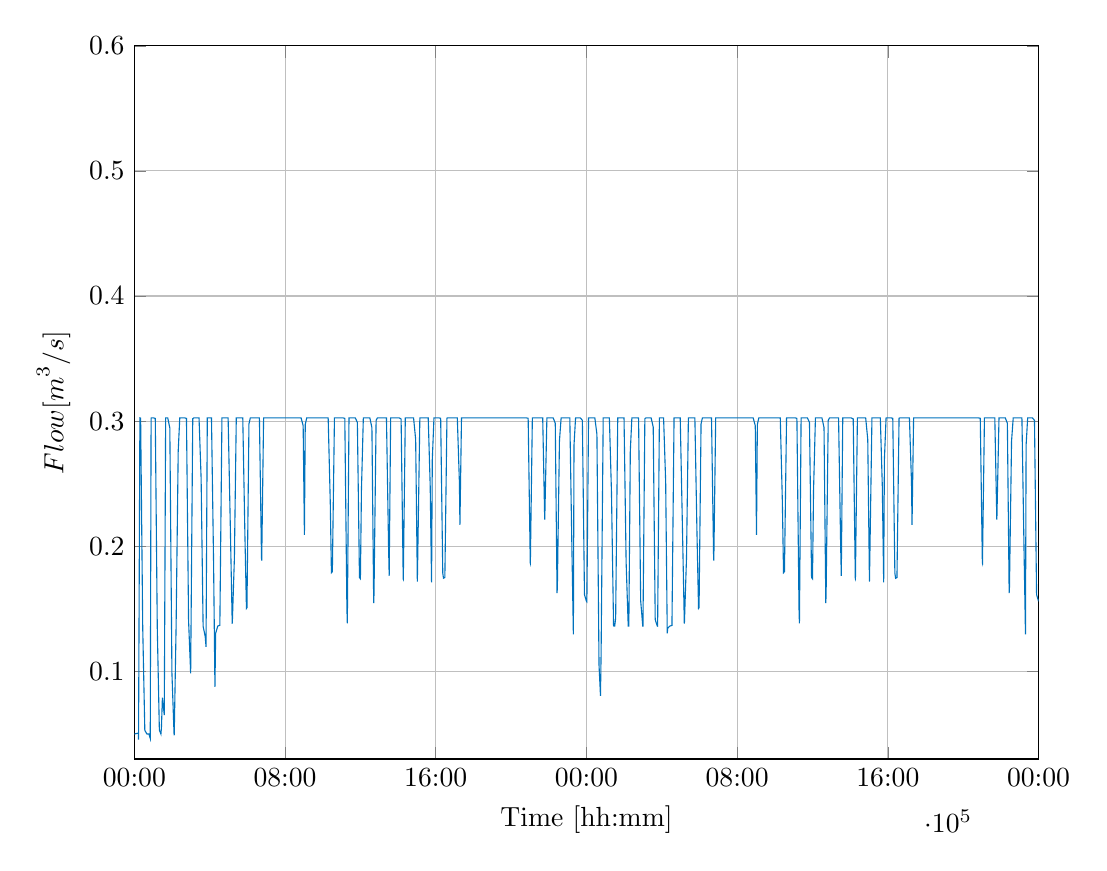
\begin{tikzpicture}

\begin{axis}[%
width=4.521in,
height=3.566in,
at={(0.758in,0.481in)},
scale only axis,
xmin=1,
xmax=172801,
xtick={1,28801,57601,86401,115201,144001,172801},
xticklabels={{00:00},{08:00},{16:00},{00:00},{08:00},{16:00},{00:00},{},{},{}},
xlabel={Time [hh:mm]},
xmajorgrids,
ymin=0.03,
ymax=0.6,
ylabel={$\text{Flow [m}^\text{3}\text{/s]}$},
ymajorgrids,
axis background/.style={fill=white}
]
\addplot [color=mycolor1,solid,forget plot]
  table[row sep=crcr]{%
1	0.0499998683647933\\
41	0.049999868172035\\
781	0.0507074272387114\\
801	0.0453941788164327\\
1061	0.302680648501631\\
1201	0.302491862717989\\
1601	0.135010674602517\\
2001	0.052887199362477\\
2401	0.0500002155001922\\
2781	0.0499999795352394\\
3041	0.0464313962055376\\
3201	0.302516352986533\\
3361	0.302680760398885\\
3601	0.302680760242387\\
4001	0.302200169403778\\
4381	0.135164719879115\\
4781	0.0530325638925076\\
5081	0.0499386124360596\\
5181	0.055586808345944\\
5361	0.0789585569468111\\
5721	0.0650508632616179\\
5981	0.302680349454319\\
6061	0.302680760387634\\
6381	0.302680760225824\\
6781	0.294520901571626\\
7181	0.0989154154146933\\
7581	0.0506834888954093\\
7621	0.0489990780965182\\
7981	0.136213836996136\\
8381	0.275956670689325\\
8681	0.302680760374472\\
8761	0.302680760242582\\
8781	0.302680760242533\\
9161	0.302680760242539\\
9561	0.302680760242384\\
9961	0.302224863193897\\
10361	0.140899783082766\\
10761	0.0983633332953129\\
11161	0.301938752023508\\
11381	0.302680760374548\\
11561	0.302680760242539\\
12081	0.302680760242539\\
12361	0.302680758907861\\
12761	0.254130778077034\\
13141	0.136059459075788\\
13541	0.127963147712897\\
13701	0.119679046615807\\
13941	0.302599210033619\\
14121	0.302680760296439\\
14341	0.302680760242539\\
14741	0.302680311240456\\
15141	0.187225056092401\\
15401	0.0875542243229154\\
15541	0.130500480790875\\
15941	0.136229862037369\\
16341	0.136809631450867\\
16741	0.302680747416122\\
16781	0.302680760373209\\
17141	0.302680760242539\\
17521	0.302680760242539\\
17921	0.302680737957046\\
18321	0.219947517927539\\
18701	0.138590577002635\\
18721	0.138604494272073\\
19121	0.190596563317006\\
19481	0.302680760292888\\
19521	0.302680760240535\\
19541	0.302680760242636\\
19921	0.302680760242539\\
20061	0.302680760242539\\
20321	0.302680760242539\\
20721	0.302680667033518\\
21121	0.210941640765384\\
21421	0.150350637668172\\
21521	0.150919846322989\\
21901	0.297770119545691\\
22161	0.302680760321777\\
22341	0.302680760242539\\
22421	0.302680760242539\\
22821	0.302680760242539\\
23001	0.302680760242539\\
23101	0.302680760242539\\
23501	0.302680760242495\\
23901	0.302537137635991\\
24301	0.190721893188483\\
24341	0.188499862099904\\
24701	0.302674453583895\\
24841	0.302680760302086\\
25101	0.302680760242539\\
25121	0.302680760242539\\
25501	0.302680760242539\\
25761	0.302680760242539\\
25901	0.302680760242539\\
25921	0.302680760242539\\
26281	0.302680760242539\\
26401	0.302680760242539\\
26681	0.302680760242539\\
26721	0.302680760242539\\
27081	0.302680760242539\\
27201	0.302680760242539\\
27481	0.302680760242539\\
27521	0.302680760242539\\
27881	0.302680760242539\\
28001	0.302680760242539\\
28281	0.302680760242539\\
28321	0.302680760242539\\
28681	0.302680760242539\\
28801	0.302680760242539\\
29081	0.302680760242539\\
29121	0.302680760242539\\
29481	0.302680760242539\\
29601	0.302680760242539\\
29881	0.302680760242539\\
29921	0.302680760242539\\
30261	0.302680760242539\\
30401	0.302680760242539\\
30661	0.302680760242539\\
30721	0.302680760242539\\
31061	0.302680760242539\\
31201	0.302680760242539\\
31461	0.302680760242539\\
31861	0.302680760226753\\
32261	0.296420028519741\\
32501	0.209173907047401\\
32661	0.297306771900499\\
32941	0.302680760303886\\
33061	0.30268076024254\\
33121	0.302680760242539\\
33461	0.302680760242539\\
33541	0.302680760242539\\
33861	0.302680760242539\\
33881	0.302680760242539\\
34261	0.302680760242539\\
34341	0.302680760242539\\
34641	0.302680760242539\\
34661	0.302680760242539\\
35041	0.302680760242539\\
35141	0.302680760242539\\
35441	0.302680760242539\\
35461	0.302680760242539\\
35841	0.302680760242539\\
35941	0.302680760242539\\
36241	0.302680760242539\\
36261	0.302680760242539\\
36641	0.302680760242539\\
37041	0.302680753339297\\
37441	0.235362546925594\\
37661	0.178862851273356\\
37841	0.179726721090916\\
38241	0.302679901182408\\
38341	0.302680760369674\\
38641	0.302680760242539\\
38681	0.302680760242539\\
39021	0.302680760242539\\
39161	0.302680760242539\\
39421	0.302680760242539\\
39821	0.302680760242383\\
40221	0.302246236787972\\
40621	0.150161908855395\\
40701	0.138355218094442\\
41021	0.302680505297797\\
41101	0.302680760397179\\
41421	0.302680760242539\\
41821	0.302680760242539\\
42221	0.302680760236874\\
42621	0.29896191150583\\
43021	0.175043157155675\\
43201	0.174045701145115\\
43401	0.245007839133707\\
43761	0.302680760291471\\
43801	0.302680760241942\\
43821	0.30268076024268\\
44201	0.302680760242539\\
44421	0.302680760242539\\
44601	0.302680760242539\\
45001	0.302680760225498\\
45401	0.294854689284065\\
45741	0.154597389404819\\
45801	0.161872632227415\\
46201	0.300594841800177\\
46461	0.302680760297433\\
46661	0.302680760242539\\
46741	0.30268076024254\\
47001	0.302680760242539\\
47121	0.302680760242539\\
47401	0.302680760242539\\
47781	0.302680760242539\\
48181	0.302679294473203\\
48581	0.200009228323768\\
48701	0.176389469603216\\
48981	0.302635857631507\\
49161	0.302680760302131\\
49441	0.30268076024254\\
49501	0.302680760242539\\
49781	0.302680760242539\\
49821	0.302680760242539\\
50181	0.302680760242539\\
50581	0.302680760241978\\
50981	0.301769350069738\\
51381	0.173914545017793\\
51401	0.173726233856688\\
51781	0.302680629822221\\
51861	0.302680760304468\\
52161	0.302680760242539\\
52201	0.302680760242539\\
52561	0.302680760242539\\
52681	0.302680760242539\\
52961	0.302680760242539\\
53361	0.302680760137084\\
53761	0.285344840884799\\
54081	0.171864139229676\\
54161	0.191627473023309\\
54561	0.302680760304719\\
54601	0.302680760241107\\
54961	0.302680760242539\\
55221	0.302680760242539\\
55361	0.302680760242539\\
55381	0.302680760242539\\
55761	0.302680760242539\\
56161	0.302680753775212\\
56541	0.248103693023625\\
56801	0.171074960948495\\
56941	0.269357952492251\\
57261	0.302680760382393\\
57361	0.302680760242545\\
57381	0.302680760242537\\
57741	0.302680760242539\\
58141	0.302680760242382\\
58541	0.302295171065643\\
58941	0.178519772866686\\
59081	0.174485379811156\\
59341	0.175023560243573\\
59741	0.302414323796332\\
59941	0.302680760295648\\
60141	0.302680760242539\\
60521	0.302680760242539\\
60921	0.302680760242539\\
61321	0.302680760242539\\
61721	0.302680757508409\\
62121	0.250916696674108\\
62221	0.217178049193355\\
62521	0.302678349363428\\
62641	0.302680760365995\\
62921	0.302680760242539\\
62941	0.302680760242539\\
63321	0.302680760242539\\
63701	0.302680760242539\\
63721	0.302680760242539\\
63861	0.302680760242539\\
64121	0.302680760242539\\
64181	0.302680760242539\\
64521	0.302680760242539\\
64661	0.302680760242539\\
64901	0.302680760242539\\
64981	0.302680760242539\\
65301	0.302680760242539\\
65321	0.302680760242539\\
65701	0.302680760242539\\
65781	0.302680760242539\\
66101	0.302680760242539\\
66121	0.302680760242539\\
66501	0.302680760242539\\
66581	0.302680760242539\\
66901	0.302680760242539\\
66921	0.302680760242539\\
67301	0.302680760242539\\
67381	0.302680760242539\\
67701	0.302680760242539\\
67721	0.302680760242539\\
68101	0.302680760242539\\
68181	0.302680760242539\\
68501	0.302680760242539\\
68521	0.302680760242539\\
68901	0.302680760242539\\
68981	0.302680760242539\\
69281	0.302680760242539\\
69301	0.302680760242539\\
69681	0.302680760242539\\
69781	0.302680760242539\\
70081	0.302680760242539\\
70101	0.302680760242539\\
70481	0.302680760242539\\
70581	0.302680760242539\\
70881	0.302680760242539\\
70901	0.302680760242539\\
71281	0.302680760242539\\
71381	0.302680760242539\\
71681	0.302680760242539\\
71701	0.302680760242539\\
72081	0.302680760242539\\
72181	0.302680760242539\\
72481	0.302680760242539\\
72501	0.302680760242539\\
72881	0.302680760242539\\
72981	0.302680760242539\\
73281	0.302680760242539\\
73301	0.302680760242539\\
73661	0.302680760242539\\
73781	0.302680760242539\\
74061	0.302680760242539\\
74101	0.302680760242539\\
74461	0.302680760242539\\
74861	0.302680760242361\\
75261	0.302311271184687\\
75661	0.18665919885132\\
75681	0.186377908093398\\
76061	0.302680540675553\\
76141	0.302680760381895\\
76461	0.302680760242539\\
76561	0.302680760242539\\
76861	0.302680760242539\\
76881	0.302680760242539\\
77261	0.302680760242539\\
77661	0.302680760242539\\
78041	0.302679346850995\\
78421	0.221375299721665\\
78441	0.222915673995048\\
78841	0.302680760370048\\
78881	0.302680760240669\\
79241	0.302680760242539\\
79341	0.302680760242539\\
79641	0.302680760242539\\
80041	0.302680760236529\\
80441	0.298307689135177\\
80781	0.162515690792454\\
80841	0.167267729521989\\
81241	0.28422427348192\\
81561	0.302680760284575\\
81641	0.302680760242527\\
81661	0.30268076024254\\
82041	0.302680760242539\\
82421	0.302680760242539\\
82841	0.302680760242539\\
83221	0.302680350128537\\
83621	0.198122368841399\\
83901	0.129520173009044\\
84021	0.280726131825289\\
84321	0.302680760283294\\
84421	0.302680760242541\\
84501	0.302680760242539\\
84961	0.302680760242539\\
85221	0.302680760240646\\
85621	0.300661703676257\\
86021	0.161380700503718\\
86401	0.155964429214595\\
86481	0.155582157734116\\
86801	0.30264576683554\\
86961	0.302680760323372\\
87201	0.302680760242539\\
87221	0.302680760242539\\
87601	0.302680760242539\\
88001	0.302680760196296\\
88401	0.289554341303737\\
88801	0.105352012864476\\
89081	0.0805055894204873\\
89201	0.114306544292461\\
89601	0.302680564793237\\
89681	0.302680760369047\\
90101	0.302680760242539\\
90301	0.302680760242539\\
90401	0.302680760242539\\
90781	0.302680757285747\\
91181	0.243263335017434\\
91581	0.136340341814795\\
91801	0.136217239567303\\
91981	0.142512616322006\\
92381	0.302680760374472\\
92421	0.302680760241047\\
92781	0.302680760242539\\
93181	0.302680760242539\\
93581	0.302679090957024\\
93981	0.187376244627345\\
94381	0.136220528223306\\
94501	0.136217239567303\\
94781	0.275956670689325\\
95081	0.302680760374472\\
95161	0.302680760242582\\
95181	0.302680760242533\\
95561	0.302680760242539\\
95961	0.302680760242503\\
96361	0.302507962825889\\
96761	0.156582670700064\\
97161	0.136217322878085\\
97201	0.136217239567303\\
97561	0.301940416259168\\
97781	0.302680760374472\\
97961	0.302680760242539\\
98061	0.302680760242539\\
98361	0.302680760242539\\
98761	0.302680760226408\\
99161	0.295215417760891\\
99541	0.141416696559254\\
99941	0.136193758336533\\
100001	0.13614720808987\\
100341	0.302668105269287\\
100481	0.302680760332779\\
100741	0.302680760242539\\
101141	0.302680758864867\\
101541	0.251403371417926\\
101841	0.130500860209357\\
101941	0.134587291476283\\
102341	0.136229862445542\\
102741	0.136809631450867\\
103141	0.302680747416122\\
103181	0.302680760373208\\
103541	0.302680760242539\\
103921	0.302680760242539\\
104321	0.302680737957046\\
104721	0.219947517927539\\
105101	0.138590577002635\\
105121	0.138604494272073\\
105521	0.190596563317006\\
105881	0.302680760292888\\
105921	0.302680760240535\\
105941	0.302680760242636\\
106321	0.302680760242539\\
106461	0.302680760242539\\
106721	0.302680760242539\\
107121	0.302680667033518\\
107521	0.210941640765384\\
107821	0.150350637668172\\
107921	0.150919846322989\\
108301	0.297770119545691\\
108561	0.302680760321777\\
108741	0.302680760242539\\
108821	0.302680760242539\\
109221	0.302680760242539\\
109401	0.302680760242539\\
109501	0.302680760242539\\
109901	0.302680760242495\\
110301	0.302537137635991\\
110701	0.190721893188483\\
110741	0.188499862099904\\
111101	0.302674453583895\\
111241	0.302680760302086\\
111501	0.302680760242539\\
111521	0.302680760242539\\
111901	0.302680760242539\\
112161	0.302680760242539\\
112301	0.302680760242539\\
112321	0.302680760242539\\
112681	0.302680760242539\\
112801	0.302680760242539\\
113081	0.302680760242539\\
113121	0.302680760242539\\
113481	0.302680760242539\\
113601	0.302680760242539\\
113881	0.302680760242539\\
113921	0.302680760242539\\
114281	0.302680760242539\\
114401	0.302680760242539\\
114681	0.302680760242539\\
114721	0.302680760242539\\
115081	0.302680760242539\\
115201	0.302680760242539\\
115481	0.302680760242539\\
115521	0.302680760242539\\
115881	0.302680760242539\\
116001	0.302680760242539\\
116281	0.302680760242539\\
116321	0.302680760242539\\
116661	0.302680760242539\\
116801	0.302680760242539\\
117061	0.302680760242539\\
117121	0.302680760242539\\
117461	0.302680760242539\\
117601	0.302680760242539\\
117861	0.302680760242539\\
118261	0.302680760226753\\
118661	0.296420028519741\\
118901	0.209173907047401\\
119061	0.297306771900499\\
119341	0.302680760303886\\
119461	0.30268076024254\\
119521	0.302680760242539\\
119861	0.302680760242539\\
119941	0.302680760242539\\
120261	0.302680760242539\\
120281	0.302680760242539\\
120661	0.302680760242539\\
120741	0.302680760242539\\
121041	0.302680760242539\\
121061	0.302680760242539\\
121441	0.302680760242539\\
121541	0.302680760242539\\
121841	0.302680760242539\\
121861	0.302680760242539\\
122241	0.302680760242539\\
122341	0.302680760242539\\
122641	0.302680760242539\\
122661	0.302680760242539\\
123041	0.302680760242539\\
123441	0.302680753339297\\
123841	0.235362546925594\\
124061	0.178862851273356\\
124241	0.179726721090916\\
124641	0.302679901182408\\
124741	0.302680760369674\\
125041	0.302680760242539\\
125081	0.302680760242539\\
125421	0.302680760242539\\
125561	0.302680760242539\\
125821	0.302680760242539\\
126221	0.302680760242383\\
126621	0.302246236787972\\
127021	0.150161908855395\\
127101	0.138355218094442\\
127421	0.302680505297797\\
127501	0.302680760397179\\
127821	0.302680760242539\\
128221	0.302680760242539\\
128621	0.302680760236874\\
129021	0.29896191150583\\
129421	0.175043157155675\\
129601	0.174045701145115\\
129801	0.245007839133707\\
130161	0.302680760291471\\
130201	0.302680760241942\\
130221	0.30268076024268\\
130601	0.302680760242539\\
130821	0.302680760242539\\
131001	0.302680760242539\\
131401	0.302680760225498\\
131801	0.294854689284065\\
132141	0.154597389404819\\
132201	0.161872632227415\\
132601	0.300594841800177\\
132861	0.302680760297433\\
133061	0.302680760242539\\
133141	0.30268076024254\\
133401	0.302680760242539\\
133521	0.302680760242539\\
133801	0.302680760242539\\
134181	0.302680760242539\\
134581	0.302679294473203\\
134981	0.200009228323768\\
135101	0.176389469603216\\
135381	0.302635857631507\\
135561	0.302680760302131\\
135841	0.30268076024254\\
135901	0.302680760242539\\
136181	0.302680760242539\\
136221	0.302680760242539\\
136581	0.302680760242539\\
136981	0.302680760241978\\
137381	0.301769350069738\\
137781	0.173914545017793\\
137801	0.173726233856688\\
138181	0.302680629822221\\
138261	0.302680760304468\\
138561	0.302680760242539\\
138601	0.302680760242539\\
138961	0.302680760242539\\
139081	0.302680760242539\\
139361	0.302680760242539\\
139761	0.302680760137084\\
140161	0.285344840884799\\
140481	0.171864139229676\\
140561	0.191627473023309\\
140961	0.302680760304719\\
141001	0.302680760241107\\
141361	0.302680760242539\\
141621	0.302680760242539\\
141761	0.302680760242539\\
141781	0.302680760242539\\
142161	0.302680760242539\\
142561	0.302680753775212\\
142941	0.248103693023625\\
143201	0.171074960948495\\
143341	0.269357952492251\\
143661	0.302680760382393\\
143761	0.302680760242545\\
143781	0.302680760242537\\
144141	0.302680760242539\\
144541	0.302680760242382\\
144941	0.302295171065643\\
145341	0.178519772866686\\
145481	0.174485379811156\\
145741	0.175023560243573\\
146141	0.302414323796332\\
146341	0.302680760295648\\
146541	0.302680760242539\\
146921	0.302680760242539\\
147321	0.302680760242539\\
147721	0.302680760242539\\
148121	0.302680757508409\\
148521	0.250916696674108\\
148621	0.217178049193355\\
148921	0.302678349363428\\
149041	0.302680760365995\\
149321	0.302680760242539\\
149341	0.302680760242539\\
149721	0.302680760242539\\
150101	0.302680760242539\\
150121	0.302680760242539\\
150261	0.302680760242539\\
150521	0.302680760242539\\
150581	0.302680760242539\\
150921	0.302680760242539\\
151061	0.302680760242539\\
151301	0.302680760242539\\
151381	0.302680760242539\\
151701	0.302680760242539\\
151721	0.302680760242539\\
152101	0.302680760242539\\
152181	0.302680760242539\\
152501	0.302680760242539\\
152521	0.302680760242539\\
152901	0.302680760242539\\
152981	0.302680760242539\\
153301	0.302680760242539\\
153321	0.302680760242539\\
153701	0.302680760242539\\
153781	0.302680760242539\\
154101	0.302680760242539\\
154121	0.302680760242539\\
154501	0.302680760242539\\
154581	0.302680760242539\\
154901	0.302680760242539\\
154921	0.302680760242539\\
155301	0.302680760242539\\
155381	0.302680760242539\\
155681	0.302680760242539\\
155701	0.302680760242539\\
156081	0.302680760242539\\
156181	0.302680760242539\\
156481	0.302680760242539\\
156501	0.302680760242539\\
156881	0.302680760242539\\
156981	0.302680760242539\\
157281	0.302680760242539\\
157301	0.302680760242539\\
157681	0.302680760242539\\
157781	0.302680760242539\\
158081	0.302680760242539\\
158101	0.302680760242539\\
158481	0.302680760242539\\
158581	0.302680760242539\\
158881	0.302680760242539\\
158901	0.302680760242539\\
159281	0.302680760242539\\
159381	0.302680760242539\\
159681	0.302680760242539\\
159701	0.302680760242539\\
160061	0.302680760242539\\
160181	0.302680760242539\\
160461	0.302680760242539\\
160501	0.302680760242539\\
160861	0.302680760242539\\
161261	0.302680760242361\\
161661	0.302311271184687\\
162061	0.18665919885132\\
162081	0.186377908093398\\
162461	0.302680540675553\\
162541	0.302680760381895\\
162861	0.302680760242539\\
162961	0.302680760242539\\
163261	0.302680760242539\\
163281	0.302680760242539\\
163661	0.302680760242539\\
164061	0.302680760242539\\
164441	0.302679346850995\\
164821	0.221375299721665\\
164841	0.222915673995048\\
165241	0.302680760370048\\
165281	0.302680760240669\\
165641	0.302680760242539\\
165741	0.302680760242539\\
166041	0.302680760242539\\
166441	0.302680760236529\\
166841	0.298307689135177\\
167181	0.162515690792454\\
167241	0.167267729521989\\
167641	0.28422427348192\\
167961	0.302680760284575\\
168041	0.302680760242527\\
168061	0.30268076024254\\
168441	0.302680760242539\\
168821	0.302680760242539\\
169241	0.302680760242539\\
169621	0.302680350128537\\
170021	0.198122368841399\\
170301	0.129520173009044\\
170421	0.280726131825289\\
170721	0.302680760283294\\
170821	0.302680760242541\\
170901	0.302680760242539\\
171361	0.302680760242539\\
171621	0.302680760240646\\
172021	0.300661703676257\\
172421	0.161380700503718\\
172801	0.155964429214595\\
};
\end{axis}
\end{tikzpicture}%
% 	%\caption{Output of the last pipe in to the WWTP, where a tank has been placed in front to reduce variation in flow into WWTP.}
% 	\label{fig:Simulering_output_second}
% 	\end{figure} 
% 	\begin{figure}[H]
% 	\centering
% 	% This file was created by matlab2tikz.
%
%The latest updates can be retrieved from
%  http://www.mathworks.com/matlabcentral/fileexchange/22022-matlab2tikz-matlab2tikz
%where you can also make suggestions and rate matlab2tikz.
%
\definecolor{mycolor1}{rgb}{0.00000,0.44700,0.74100}%
%
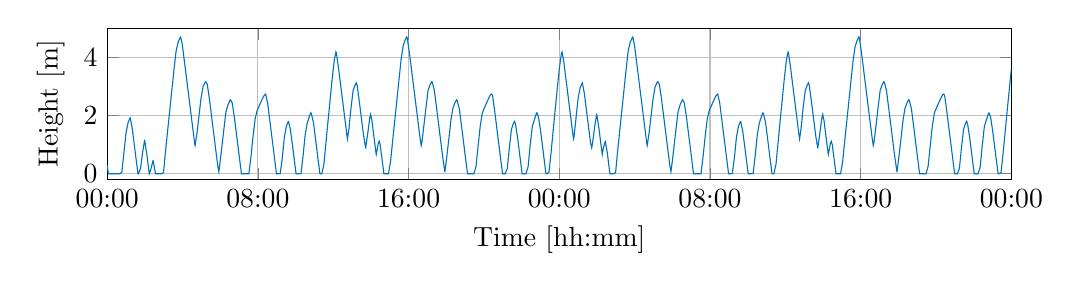
\begin{tikzpicture}

\begin{axis}[%
width=4.521in,
height=.7566in,
at={(0.758in,0.481in)},
scale only axis,
xmin=1,
xmax=172801,
xtick={1,28801,57601,86401,115201,144001,172801},
xticklabels={{00:00},{08:00},{16:00},{00:00},{08:00},{16:00},{00:00},{},{},{}},
xlabel={Time [hh:mm]},
xmajorgrids,
ymin=-0.2,
ymax=5,
scaled x ticks = false,
ylabel={Height [m]},
ymajorgrids,
axis background/.style={fill=white}
]
\addplot [color=mycolor1,solid,forget plot]
  table[row sep=crcr]{%
1	0.3\\
221	0\\
401	0\\
801	0\\
1201	0\\
1601	0\\
2001	0\\
2401	0\\
2801	0.0477309745637752\\
3201	0.719918364876453\\
3601	1.40407479606802\\
4001	1.76469357714613\\
4381	1.92351364981831\\
4401	1.92587639924579\\
4781	1.57488558210966\\
5181	1.00046250972562\\
5581	0.425681155957782\\
5881	0\\
5981	0\\
6381	0.189924867423544\\
6781	0.748476659417658\\
7141	1.13940178305009\\
7181	1.13163641507966\\
7581	0.660584293688091\\
7981	0.0858442719532861\\
8041	0\\
8381	0.182768655519709\\
8761	0.451336422519302\\
8781	0.452920979421766\\
9161	0.078517738570607\\
9221	0\\
9561	0\\
9961	0\\
10361	0\\
10761	0.0377955999006336\\
11161	0.79716026542577\\
11561	1.48908605165114\\
11961	2.18097136454189\\
12361	2.87285667743263\\
12761	3.56474199031781\\
13141	4.18146617918322\\
13541	4.51489441225188\\
13941	4.67356007543898\\
14041	4.69802986849243\\
14341	4.45741476945105\\
14741	3.8858239105959\\
15141	3.31104255713799\\
15541	2.73626120336206\\
15941	2.16147984958614\\
16341	1.58669849581021\\
16741	1.01303469647034\\
16801	0.972551566855012\\
17141	1.36060373120019\\
17521	1.95456133391272\\
17921	2.5748211268253\\
18321	2.99165369969557\\
18721	3.14716373341218\\
18821	3.16168545689058\\
19121	3.077792659826\\
19521	2.58784517239249\\
19921	2.01307204618232\\
20321	1.43829069240645\\
20721	0.86350933863053\\
21121	0.28902465093073\\
21341	0.0702088332853154\\
21521	0.314753121487285\\
21901	0.889718633810231\\
22301	1.52893279427028\\
22701	2.12835052680236\\
23101	2.37499768308534\\
23501	2.52997076752696\\
23581	2.54151664983667\\
23901	2.42397474965734\\
24301	1.94519891018198\\
24701	1.37043486855995\\
25101	0.795653514784177\\
25501	0.220872161008255\\
25661	0\\
25901	0\\
26281	0\\
26681	0\\
27081	0\\
27481	0.5923443520069\\
27881	1.28320670566423\\
28281	1.88580382740198\\
28681	2.18474073510185\\
29081	2.34329896155424\\
29481	2.50185094111165\\
29881	2.66037570866542\\
30261	2.73912621868908\\
30281	2.73947796503749\\
30661	2.42797560060844\\
31061	1.85430085744476\\
31461	1.27951950371784\\
31861	0.704738149941915\\
32261	0.129956796165993\\
32361	0\\
32661	0\\
33061	0.00264896273383396\\
33461	0.536754838158371\\
33861	1.26125247936649\\
34261	1.64876541294607\\
34641	1.80092878646541\\
34661	1.80100081777591\\
35041	1.48242823435999\\
35441	0.937304911333102\\
35841	0.362524294648796\\
36101	0\\
36241	0\\
36641	0\\
37041	0.00554233182095331\\
37441	0.616832267364113\\
37841	1.34201297598632\\
38241	1.74635010322595\\
38641	1.97156852844576\\
38921	2.09339139435165\\
39021	2.06594208715208\\
39421	1.75958460953669\\
39821	1.19385215597759\\
40221	0.619070806349016\\
40621	0.0442894525730948\\
40661	0\\
41021	0\\
41421	0.330813811111981\\
41821	1.08617020522357\\
42221	1.84353702724792\\
42621	2.57114709027542\\
43021	3.29594298357653\\
43401	3.90326435749542\\
43721	4.18416483600051\\
43801	4.15371296898687\\
44201	3.64481073936533\\
44601	3.07003123388912\\
45001	2.49524988011321\\
45401	1.92046852633728\\
45801	1.34568811296343\\
45921	1.19688493097295\\
46201	1.54130476204739\\
46601	2.26542646476012\\
47001	2.86264075194371\\
47401	3.0508511106173\\
47601	3.12276133021875\\
47781	3.03043759024906\\
48181	2.4847380073981\\
48581	1.9099567638187\\
48981	1.33517541022276\\
49381	0.898572117451366\\
49401	0.893064813522904\\
49781	1.36226549174542\\
50181	1.91777594110188\\
50341	2.03246659657299\\
50581	1.83571788425917\\
50981	1.26626864033144\\
51381	0.700965084288649\\
51421	0.662897235514634\\
51781	1.01988330579652\\
51981	1.1158182149364\\
52161	1.00698127950694\\
52561	0.454215584163409\\
52881	0\\
52961	0\\
53361	0\\
53761	0\\
54161	0.427390145820136\\
54561	1.14314339525267\\
54961	1.83502870809652\\
55361	2.52691402098726\\
55761	3.21879933387801\\
56161	3.91051340633468\\
56541	4.37597879991354\\
56941	4.59494103083462\\
57241	4.69802986849243\\
57341	4.67015418222383\\
57741	4.17321049493022\\
58141	3.59843323402592\\
58541	3.02365188025002\\
58941	2.4488705264741\\
59341	1.87408917269818\\
59741	1.29930781892238\\
60001	0.972551566855012\\
60141	1.0755196315864\\
60521	1.64195201080034\\
60921	2.26715827535808\\
61321	2.86096028187479\\
61721	3.07097045261734\\
62021	3.16168545689058\\
62121	3.14631204760874\\
62521	2.87072720537462\\
62921	2.30046272239251\\
63321	1.72568136929441\\
63721	1.15090001551849\\
64121	0.57611866178788\\
64521	0.072353301853959\\
64541	0.0702088332853154\\
64901	0.587101524444758\\
65301	1.20005017833556\\
65701	1.85803510021502\\
66101	2.27211799313536\\
66501	2.4543332602539\\
66781	2.54151664983667\\
66901	2.51314846900908\\
67301	2.22606146819156\\
67701	1.65782554378044\\
68101	1.08304419167214\\
68501	0.508262837896216\\
68861	0\\
68901	0\\
69281	0\\
69681	0\\
70081	0\\
70481	0.246401691044499\\
70881	0.938286919375952\\
71281	1.6193263095909\\
71681	2.08064009446333\\
72081	2.26402297177554\\
72481	2.42257495133295\\
72881	2.58112693088985\\
73281	2.72345684022445\\
73481	2.73947796503749\\
73661	2.66925982102245\\
74061	2.14169086579945\\
74461	1.56691018060579\\
74861	0.992128826829875\\
75261	0.417347473053954\\
75561	0\\
75661	0\\
76061	0\\
76461	0.174195287808284\\
76861	0.899364161006185\\
77261	1.52616681059574\\
77661	1.74429924759959\\
77861	1.80100081777591\\
78041	1.69898866065651\\
78441	1.22372150743432\\
78841	0.649914971474737\\
79241	0.0751336177608396\\
79301	0\\
79641	0\\
80041	0\\
80441	0.236617136315758\\
80841	0.979692026608217\\
81241	1.62576547087511\\
81641	1.85895942642209\\
82041	2.07795150400339\\
82121	2.09339139435165\\
82421	1.95229956897995\\
82821	1.48120817919515\\
83221	0.906461483236618\\
83621	0.331680129461056\\
83861	0\\
84021	0\\
84421	0.0442320015654817\\
84821	0.706894211091728\\
85221	1.46544614770521\\
85621	2.20853775072044\\
86021	2.93375641290547\\
86401	3.59782298159265\\
86801	4.13020275125589\\
86921	4.18416483600051\\
87201	3.93013179319851\\
87601	3.3574219106404\\
88001	2.78264055700117\\
88401	2.20785920322525\\
88801	1.63307784944932\\
89121	1.19688493097295\\
89201	1.24461590553673\\
89601	1.91680329584941\\
90001	2.60095972704098\\
90401	2.96157850811909\\
90781	3.12039858079127\\
90801	3.12276133021875\\
91181	2.77177051308261\\
91581	2.19734744069857\\
91981	1.62256608693074\\
92381	1.04895928428749\\
92601	0.893064813522904\\
92781	1.08298968094645\\
93181	1.64154147294056\\
93541	2.03246659657299\\
93581	2.02470122860257\\
93981	1.553649107211\\
94381	0.97890908547619\\
94621	0.662897235514634\\
94781	0.845665891034342\\
95161	1.11423365803394\\
95181	1.1158182149364\\
95561	0.741414974085241\\
95961	0.16682495019045\\
96081	0\\
96361	0\\
96761	0\\
97161	0.0377955999006336\\
97561	0.79716026542577\\
97961	1.48908605165114\\
98361	2.18097136454189\\
98761	2.87285667743263\\
99161	3.56474199031781\\
99541	4.18146617918322\\
99941	4.51489441225188\\
100341	4.67356007543898\\
100441	4.69802986849243\\
100741	4.45741476945105\\
101141	3.8858239105959\\
101541	3.31104255713799\\
101941	2.73626120336206\\
102341	2.16147984958614\\
102741	1.58669849581021\\
103141	1.01303469647034\\
103201	0.972551566855012\\
103541	1.36060373120019\\
103921	1.95456133391272\\
104321	2.5748211268253\\
104721	2.99165369969557\\
105121	3.14716373341218\\
105221	3.16168545689058\\
105521	3.077792659826\\
105921	2.58784517239249\\
106321	2.01307204618232\\
106721	1.43829069240645\\
107121	0.86350933863053\\
107521	0.28902465093073\\
107741	0.0702088332853154\\
107921	0.314753121487285\\
108301	0.889718633810231\\
108701	1.52893279427028\\
109101	2.12835052680236\\
109501	2.37499768308534\\
109901	2.52997076752696\\
109981	2.54151664983667\\
110301	2.42397474965734\\
110701	1.94519891018198\\
111101	1.37043486855995\\
111501	0.795653514784177\\
111901	0.220872161008255\\
112061	0\\
112301	0\\
112681	0\\
113081	0\\
113481	0\\
113881	0.5923443520069\\
114281	1.28320670566423\\
114681	1.88580382740198\\
115081	2.18474073510185\\
115481	2.34329896155424\\
115881	2.50185094111165\\
116281	2.66037570866542\\
116661	2.73912621868908\\
116681	2.73947796503749\\
117061	2.42797560060844\\
117461	1.85430085744476\\
117861	1.27951950371784\\
118261	0.704738149941915\\
118661	0.129956796165993\\
118761	0\\
119061	0\\
119461	0.00264896273383396\\
119861	0.536754838158371\\
120261	1.26125247936649\\
120661	1.64876541294607\\
121041	1.80092878646541\\
121061	1.80100081777591\\
121441	1.48242823435999\\
121841	0.937304911333102\\
122241	0.362524294648796\\
122501	0\\
122641	0\\
123041	0\\
123441	0.00554233182095331\\
123841	0.616832267364113\\
124241	1.34201297598632\\
124641	1.74635010322595\\
125041	1.97156852844576\\
125321	2.09339139435165\\
125421	2.06594208715208\\
125821	1.75958460953669\\
126221	1.19385215597759\\
126621	0.619070806349016\\
127021	0.0442894525730948\\
127061	0\\
127421	0\\
127821	0.330813811111981\\
128221	1.08617020522357\\
128621	1.84353702724792\\
129021	2.57114709027542\\
129421	3.29594298357653\\
129801	3.90326435749542\\
130121	4.18416483600051\\
130201	4.15371296898687\\
130601	3.64481073936533\\
131001	3.07003123388912\\
131401	2.49524988011321\\
131801	1.92046852633728\\
132201	1.34568811296343\\
132321	1.19688493097295\\
132601	1.54130476204739\\
133001	2.26542646476012\\
133401	2.86264075194371\\
133801	3.0508511106173\\
134001	3.12276133021875\\
134181	3.03043759024906\\
134581	2.4847380073981\\
134981	1.9099567638187\\
135381	1.33517541022276\\
135781	0.898572117451366\\
135801	0.893064813522904\\
136181	1.36226549174542\\
136581	1.91777594110188\\
136741	2.03246659657299\\
136981	1.83571788425917\\
137381	1.26626864033144\\
137781	0.700965084288649\\
137821	0.662897235514634\\
138181	1.01988330579652\\
138381	1.1158182149364\\
138561	1.00698127950694\\
138961	0.454215584163409\\
139281	0\\
139361	0\\
139761	0\\
140161	0\\
140561	0.427390145820136\\
140961	1.14314339525267\\
141361	1.83502870809652\\
141761	2.52691402098726\\
142161	3.21879933387801\\
142561	3.91051340633468\\
142941	4.37597879991354\\
143341	4.59494103083462\\
143641	4.69802986849243\\
143741	4.67015418222383\\
144141	4.17321049493022\\
144541	3.59843323402592\\
144941	3.02365188025002\\
145341	2.4488705264741\\
145741	1.87408917269818\\
146141	1.29930781892238\\
146401	0.972551566855012\\
146541	1.0755196315864\\
146921	1.64195201080034\\
147321	2.26715827535808\\
147721	2.86096028187479\\
148121	3.07097045261734\\
148421	3.16168545689058\\
148521	3.14631204760874\\
148921	2.87072720537462\\
149321	2.30046272239251\\
149721	1.72568136929441\\
150121	1.15090001551849\\
150521	0.57611866178788\\
150921	0.072353301853959\\
150941	0.0702088332853154\\
151301	0.587101524444758\\
151701	1.20005017833556\\
152101	1.85803510021502\\
152501	2.27211799313536\\
152901	2.4543332602539\\
153181	2.54151664983667\\
153301	2.51314846900908\\
153701	2.22606146819156\\
154101	1.65782554378044\\
154501	1.08304419167214\\
154901	0.508262837896216\\
155261	0\\
155301	0\\
155681	0\\
156081	0\\
156481	0\\
156881	0.246401691044499\\
157281	0.938286919375952\\
157681	1.6193263095909\\
158081	2.08064009446333\\
158481	2.26402297177554\\
158881	2.42257495133295\\
159281	2.58112693088985\\
159681	2.72345684022445\\
159881	2.73947796503749\\
160061	2.66925982102245\\
160461	2.14169086579945\\
160861	1.56691018060579\\
161261	0.992128826829875\\
161661	0.417347473053954\\
161961	0\\
162061	0\\
162461	0\\
162861	0.174195287808284\\
163261	0.899364161006185\\
163661	1.52616681059574\\
164061	1.74429924759959\\
164261	1.80100081777591\\
164441	1.69898866065651\\
164841	1.22372150743432\\
165241	0.649914971474737\\
165641	0.0751336177608396\\
165701	0\\
166041	0\\
166441	0\\
166841	0.236617136315758\\
167241	0.979692026608217\\
167641	1.62576547087511\\
168041	1.85895942642209\\
168441	2.07795150400339\\
168521	2.09339139435165\\
168821	1.95229956897995\\
169221	1.48120817919515\\
169621	0.906461483236618\\
170021	0.331680129461056\\
170261	0\\
170421	0\\
170821	0.0442320015654817\\
171221	0.706894211091728\\
171621	1.46544614770521\\
172021	2.20853775072044\\
172421	2.93375641290547\\
172801	3.59782298159265\\
};
\end{axis}
\end{tikzpicture}%
% 	%\caption{Output of the last pipe in to the WWTP, where a tank has been placed in front to reduce variation in flow into WWTP.}
% 	\label{fig:Simulering_output_second_height}
% 	\end{figure} 
% \end{frame}


 \section{Diskussion/Konklusion}
% \begin{frame}{Diskussion}{}
% 	\vfill \vfill \centering
% 	\begin{itemize}

% 	%	\item Wastewater of Aerobic/Anaerobic Transformations in Sewers (WATS)
% 	\end{itemize}
% 	\vfill \vfill
% \end{frame}

%\section{}

\begin{frame}{Diskussion/Konklusion}{}
	\vfill \vfill\centering
	\begin{itemize}
			\item Courant's tal
			\item Model reduktion
	    	\item Simulering
	    	%\item MPC
	\end{itemize}    

	\vfill \vfill
\end{frame}
